                                                                                                                                                                                                                                                                                                                                  %% ----- PREAMBLE
\documentclass[a4paper,12pt,oneside,openany,fleqn]{uerj}

%% ----- FONTSTYLE
 %\usepackage[adobe-utopia]{mathdesign} 
\usepackage{fourier} % nicer math font style
\newcommand{\textarray}[1]{\ensuremath{\left[ \mbox{\ttfamily\begin{tabular}{c} #1 \end{tabular}}\right]}}
\usepackage{tikz}
\usetikzlibrary{patterns}
\usepackage{relsize}
\usetikzlibrary{shapes,arrows,arrows.meta,matrix}
\usepackage{pdfpages}



% # Remark: Uncomment these two lines below to have Arial font in the worst case 
% 				   (UERJ's original horrible font). Owing to change of font, the footer of the title page 
%                 might leak out from the page. 
%\usepackage{helvet}
%\renewcommand{\familydefault}{\sfdefault}

%% ----- NOMENCLATURE (optional)
% Remark: the code below sorts the nomenclature in subgroups. 
%			    To have your symbols organized accordingly, use something 
% 				like the following throughout the text, provided that 'g','r','u','d','x' 
%				are kept as initial letters:
%
% 						\nomenclature[g]{$ \alpha $}{Some greek constant}
% 						\nomenclature[r]{$ t $}{Some roman variable}
% 						\nomenclature[x]{$ ( . , .) $}{Some roman variable}
%
% 				If a nomenclature section is not intended, comment all the lines. 
%
\makeindex
\makenomenclature % nomenclature
\RequirePackage{ifthen}
 \renewcommand\nomgroup[1]{%
   \ifthenelse{\equal{#1}{A}}{%
    \item[\textbf{Acronyms}] }{% A - Acronyms
     \ifthenelse{\equal{#1}{R}}{%
      \item[\textbf{Roman letters}]}{% R - Roman
       \ifthenelse{\equal{#1}{G}}{%
        \item[\textbf{Greek letters }]}{% G - Greek
         \ifthenelse{\equal{#1}{S}}{%
          \item[\textbf{Superscripts}]}{{% S - Superscripts
       \ifthenelse{\equal{#1}{U}}{%
        \item[\textbf{Subscripts }]}{{% U - Subscripts
         \ifthenelse{\equal{#1}{X}}{%
          \item[\textbf{Symbols}]}% X - Other Symbols
                    {{}}}}}}}}}} 

    
%% ----- TABLE FOOTNOTE COUNTER
\newcounter{tablenote}[table]
\newcommand{\itemx}[1]{
    \stepcounter{tablenote}
    \item[\thetablenote]\label{#1} }

%% ----- CUSTOMIZATION
\numberwithin{equation}{chapter}
\theoremstyle{plain}

% # Remark: options to redefine caption names, since Babel overwrites 
%				   definitions inside file .cls. Comment, in case of Portuguese.
%
%				   Useful options:
%								\appendixname	 Appendix
%								\bibname	 		 Bibliography (report,book)
%								\contentsname	 Contents
%								\figurename	 	 Figure (for captions)
%								\indexname	 	 Index
%								\listfigurename	 List of Figures
%								\listtablename	 List of Tables
%\pagename	 	 	 Page (letter)
%\refname	 	 	 References (article)
%\seename	 		 see (makeidx package)
%\tablename	 	 	Table (for caption)
\captionsetup[figure]{name=Figure}
\captionsetup[table]{name=Table}

%% ----- SETUP FOR REFERENCES
% 	# Remark: package 'cleveref' (pre-loaded) enables intelligent cross-referencing. 
%					however it was buggy for figure environments. 
%				    (See http://www.ctan.org/pkg/cleveref) 
%
% # Remark: the suggested use of cross-referencing is:
% 				   \cref{} for equations, sections, subsections, and chapters;
% 				   \ref{} for figures and tables;
%
% # Remark: appendices need to be written manually since the lettered 
%				   titles are not optimized for cross-reference.
%
\crefname{equation}{Equation}{Equations} % {kind}{label_singular}{label_plural}
\crefname{chapter}{Chapter}{Chapters}
\crefname{appendix}{Appendix}{Appendix}
\crefname{figure}{Figure}{Figures}
\crefname{section}{Section}{Sections}
\crefname{subsection}{Subsection}{Subsections}

%% -----  HYPERREF
% Changing standard \autoref label printing:
\renewcommand*{\tableautorefname}{Table}


%% ----- USER-DEFINED COMMANDS
% Here you may wish define your own commands
\newcommand{\Etal}{\emph{et al.}}

%% ----- HYPHENATION
% Use this command to teach words to LaTex. 
\hyphenation{en-ge-nha-ri-a}

%% ----- BEGIN OF DOCUMENT

\begin{document}

%% ----- MARKUP REFERENCES SETUPS  
% Change the values to have coloured links 
% (maybe useful for draft version or correction purposes): 
%			e.g. 'colorlinks=true', 'linkcolor=red', 'citecolor=blue', etc.
\hypersetup{    
    %colorlinks=false,    
    citecolor=black,
    filecolor=black,
    linkcolor=black,
    urlcolor=black,
    linktoc=all,   
}

%% ----- PRE-TEXTUAL ELEMENTS  (SECTION 00)
\thispagestyle{empty}\begin{titlepage}
\begin{center}

	\vspace{-0.5cm}

  \begin{figure}[hbt!]
		\begin{flushleft}
		   
\includegraphics[width=3.44cm,height=3.17cm]{logos/logo_uerj_bw}
		\end{flushleft}
	\end{figure}
	\vspace{-4cm}

  \hspace{2cm}\large{\textbf{Universidade do Estado do Rio de Janeiro}}\\
  \hspace{2cm}\large{Centro de Tecnologia e Ciências}\\
  \hspace{2cm}\large{Faculdade de Engenharia}\\

  \hspace{2cm}\large{}\\
  \hspace{2cm}\large{}\\
  \hspace{2cm}\large{}\\
  \hspace{2cm}\large{}\\

  \par
  \Large{Leandro Marques dos Santos}

  \hspace{2cm}\large{}\\
  \hspace{2cm}\large{}\\
  \hspace{2cm}\large{}\\
  \hspace{2cm}\large{}\\


  \par
  \textbf{\LARGE An ALE-FE Method for Blood Flow Dynamics in Coronary Arteries Using the Vorticity-Streamfunction Formulation}

  \par\vfill
  {\large Rio de Janeiro, Brazil\\2020}

\end{center}
\end{titlepage}

\pagebreak\thispagestyle{empty}\begin{center}

{\large Leandro Marques dos Santos}

% \vfill
\vspace{2cm}

\textbf{\LARGE 
An ALE-FE Method for Blood Flow Dynamics in Coronary Arteries Using the Vorticity-Streamfunction Formulation}

\vspace{1.0cm}

\begin{figure}[hbt!]
\begin{center}

\includegraphics[width=10.48cm,height=10.8cm]{logos/logo_uerj_mark}
\end{center}
\end{figure}

\vspace{-9cm}
\begin{flushright}
\parbox{8cm}{
\singlespacing{\large Master's Thesis presented to the Mechanical Engineering Graduate Program of State University of Rio de Janeiro (UERJ) as a partial requirement to obtain the degree of Master in Sciences. \linebreak Field of concentration: Transport Phenomena.} 
}
\end{flushright}

\vspace{4.0cm}

{\large Advisor: Prof. Gustavo Rabello dos Anjos, Ph.D.\\
        Co-Advisor: Prof. José da Rocha Miranda Pontes, D.Sc.}\\

\par\vfill
%\vspace{2cm}

{\large Rio de Janeiro, Brazil\\2020}

\end{center}

\pagebreak\thispagestyle{empty}% Guideline:
% 		After finishing your paperwork, you should send a PDF of this page to the Library CTC/B at UERJ so that they check the data and 
%		approve the catalog sheet. Check the CTC/B website for updated contacts. Otherwise talk to the librarian personally. 
\begin{titlepage}
	\begin{center}
\vfill
\singlespacing
	\vspace*{85mm}
	{CATALOGAÇÃO NA FONTE\\ \vspace{1.5mm}
	UERJ\,/\,REDE SIRIUS\,/\,BIBLIOTECA CTC/B}\\
	\vspace{1.5mm}
	\begin{boxedminipage}{140mm}
	\begin{minipage}{5mm}
		\vspace{-80mm}
		S237
	\end{minipage}
	\hfill
	\raisebox{8.5mm}{
	\begin{minipage}[top]{115mm}
		\vspace*{5mm}

		Sobrenome, Nome\\
		\phantom{XX}Titulo Dissertação \,/\,Nome e Sobrenome -- 2020.\\
		\phantom{XX}138\,f.\\
		\phantom{XX}\\
		\phantom{XX}Orientador: Nome e Sobrenome\\
%\hspace*{5mm}
       		\phantom{XX}Dissertação apresentada, como requisito parcial para obtenção do tı́tulo de Mestre em Ciências, ao Programa de Pós-Graduação em Engenharia Mecânica da Universidade do Estado do Rio de Janeiro. Área da concentração: Fenômenos de Transporte\\
%       	\phantom{XX} Bibliografia: f.159-176.
		\phantom{XX}\\
		\phantom{XX}XXXXXXXXXXXXXXXXXXXXXXXXXXXXXXXXXXXXXXXXXXXXX.
%                \phantom{XX}Texto a ser informado pela biblioteca.
	\end{minipage}}
	\vspace*{5mm}
	\begin{flushright}
	 CDU 621
	\end{flushright}
    \vspace{1mm}
	\end{boxedminipage}\\
	\end{center}
\vspace{1cm}
	Autorizo, apenas para fins acadêmicos e científicos, a reprodução total ou parcial desta dissertação, desde que citada a fonte.\\
	\noindent
	\begin{tabular}{ccc}
	\phantom{XXXXXXXXXXXXXXXXXXXXXXXXXXXXXX}&	 \phantom{XX}	&	\phantom{XXXXXXXXXXXXXXXX}	\\
	\phantom{XXXXXXXXXXXXXXXXXXXXXXXXXXXXXX}&	 \phantom{XX}	&	\phantom{XXXXXXXXXXXXXXXX}	\\
	\cline{1-1}\cline{3-3}
	Assinatura &		&	Data
	\end{tabular}
\end{titlepage} 
   
\pagebreak\thispagestyle{empty}\addtocounter{page}{+1}
\begin{center}

{\large Leandro Marques dos Santos}

\vspace{1cm}

\textbf{\large Simulação Numérica em Elementos Finitos do Escoamento em Artéria Coronária}

\end{center}

\vspace{.4cm}

\begin{flushright}
\parbox{8cm}{
\singlespacing{Trabalho de conclusão de curso apresentado como requisito parcial para obtenção do título de Bacharel em Engenharia Mecânica da Universidade do Estado do Rio de Janeiro.}
}
\end{flushright}

\vspace{.6cm}

% Date of defense; if not completed, leave it blank.
\noindent Aprovado em: 10 de Setembro de 2018

% Jury: UERJ's professors MUST BE come first, regardless whoever.
\noindent Banca Examinadora:

\vspace{.7cm}

\begin{flushright}
\parbox{12cm}{

\singlespacing

\hrulefill \\

\vspace{-.4cm}
Prof. D.Sc. Gustavo Rabello dos Anjos (Orientador)
\newline
Faculdade de Engenharia - UERJ
\vspace{.7cm}

\hrulefill \\

\vspace{-.4cm}
Prof. D.Sc. José da Rocha Miranda Pontes (Co-orientador)
\newline
Faculdade de Engenharia - UERJ
\vspace{.7cm}

\hrulefill \\

\vspace{-.4cm}
D.Sc. Rachel Manhães de Lucena
\newline
Faculdade de Engenharia - UERJ
\vspace{.7cm}

\hrulefill \\

\vspace{-.4cm}
Prof. D.Sc. Fabio Pereira dos Santos
\newline
Universidade Federal do Rio de Janeiro - UFRJ
\vspace{.7cm}

}
\end{flushright}
\vfill

\begin{center}
Rio de Janeiro\linebreak 2018
\end{center}


%\pagebreak\thispagestyle{empty}\begin{center}
\textbf{DEDICATION}
\end{center}

$\!$\\

%\vspace{1cm}
\null
\vfill
\begin{center}
\noindent I dedicate this thesis to my garden's lily, natural beauty, spring of my inspiration. To you, wholeheartedly. 
\end{center}




\pagebreak\thispagestyle{empty}\begin{center}
\textbf{ACKNOWLEDGMENTS}
\end{center}
$\!$\\

\medskip 
This work was developed at the Numerical Simulations Laboratory (LEN) of the Environmental Simulations in Reservoirs and Study Group (GESAR) of State University of Rio de Janeiro (UERJ).

\medskip 
Initially, I would like to record my gratitude and great admiration for my advisor, Prof. Gustavo Rabello dos Anjos, for his teachings, instructions and attention in preparing this work and in my development.
Also, I would like to thank my co-Advisor Prof. José da Rocha Miranda Pontes for the support and development in my academic background.
To the Gesar Research Group, in particular to Prof. Norberto Mangiavacchi for providing all infrastructure necessary for the elaboration of this work and his dedication in the graduate program where this work was performed. Moreover, to Prof. Gustavo Oliveira and Rachel Lucena for their contribuitions in this work.

\medskip 
My thanks to my colleagues of LEN, Livia Correa, Luis Carnevale, Haroldo Rufino, Gabriel Oliveira, Leonardo Paiva and Daniel Coelho, for contributing in several ways to complete this goal and make my days more pleasant.

\medskip 
To my family for all encouragement and support. To my parents, Ana Marques and Edson Santos, for careful. To my brother, Pedro Marques, for friendship. To my wife, Leticia Marques, whom this work is dedicated, for all attention, encouragement and friendship.

\medskip 
In particular, to the Creator, whom provides the inspiration.

%\pagebreak\thispagestyle{empty}$\!$\\

\null
\vfill
\begin{flushright}
In the midst of chaos, there is also opportunity.  \\
\vspace{0.5cm}
\textit{Sun Tzu, The Art of War}
\end{flushright}

\thispagestyle{empty}


\pagebreak\thispagestyle{empty}\begin{center}
\textbf{ABSTRACT}
\end{center}

% JUST ONE paragraph.
% Number of sheets (NS) = PDF pages - 2 (less cover and 2 first pages, which are printed at the same sheet)

$\!$\\

\hspace{-1.3cm}\textbf{Marques}, Leandro \textit{An ALE-FE Method for Vorticity-Streamfunction Formulation with Species Transport Equation}. xxf. Master's Thesis~(Master of Mechanical Engineering) - Engineering Departament, State University of Rio de Janeiro~(UERJ), Rio de Janeiro, Brazil, 2020.

\vspace{.2cm}

\indent The present work aims at developing a computational framework to simulate blood flow in coronary artery with
drug-eluting stent placed using Vorticity-Streamfunction Formulation in an Arbitrary Lagrangian-Eulerian (ALE) approach.
The blood was modeled as single-phase, incompressible and newtonian fluid and. The Navier-Stokes equation is shown according to the vorticity-streamfunction formulation with pecies transport equation.
The Finite Element Method (FEM) is used to solve the governing equations where the Galerkin formulation was used
to discretized the equations in space and the semi-Lagrangian method was used to discretized the material derivative
using first order backward difference scheme. The linear systems was solved using Conjugate Gradient Iterative Method.

\vspace{1cm}

\hspace{-1.3cm}Keywords: Abritary Lagrangian-Eulerian; Vorticity-Streamfunction Formulation; Finite Element Method; semi-Lagrangian Method; Drug-Eluting Stent.

\pagebreak\thispagestyle{empty}d\begin{center}
\textbf{RESUMO}
\end{center}

% JUST ONE paragraph.
% Number of sheets (NS) = PDF pages - 2 (less cover and 2 first pages, which are printed at the same sheet)

$\!$\\

\hspace{-1.3cm}MARQUES, Leandro \textit{Um Método FE-ALE para a Dinâmica do Escoamento Sanguíneo na Artéria Coronária Usando a Formulação Corrente-Vorticidade}. 99f. Dissertação de Mestrado (Mestrado em Engenharia Mecânica) - Faculdade de Engenharia, Universidade do Estado do Rio de Janeiro~(UERJ), Rio de Janeiro, Brasil, 2020.

\vspace{.2cm}

\indent 
O presente trabalho tem como objetivo o desenvolvimento 
de uma estrutura computacional para simular o escoamento 
sanguíneo em uma artéria coronária com stent farmacológico 
implantado para diversos números de Schmidt usando a Formulação Corrente-Vorticidade em uma 
abordagem Lagrangeana-Euleriana Arbitrária (ALE).
O fluido sanguíneo foi modelado como incompressível e newtoniano em um escolamento monofásico.
A equação de Navier-Stokes é apresentada segundo a formulação 
corrente-vorticidade com a equação de transporte de espécie química.
O Método dos Elementos Finitos (FEM) é usado para resolver as equações 
de governo, onde a formulação de Galerkin foi usada para 
discretização no espaço, enquanto o Método semi-Lagrangeano 
foi usado para discretizar a derivada material usando 
o \textit{backward difference scheme}. 
Além disso, o procedimento de remalhamento
realiza a regularização dos nós possibilitando
simular problemas com contornos móveis e os sistemas lineares foram resolvidos utilizando o 
Método Iterativo Gradientes Conjugados.
Portanto, a nova formulação proposta
nesse trabalho é apropriada para
simular escoamentos em artéria coronária com boa precisão.

\vspace{1cm}

\hspace{-1.3cm}Palavras-chave: Lagrangeana-Euleriana Arbitrária; Formulação Corrente-Vorticidade; Método dos Elementos Finitos; Método semi-Lagrangeano; Stent Farmacológico.


\fancypagestyle{plain}{
\fancyhf{} % clear all header and footer fields
\renewcommand{\headrulewidth}{0pt}
\renewcommand{\footrulewidth}{0pt}}
\pagestyle{plain}

\pagebreak

%% ----- LISTS  

%% LIST OF FIGURES
\def\listfigurename{LIST OF FIGURES}\listoffigures

%% LIST OF TABLES
\def\listtablename{LIST OF TABLES}\listoftables

%% LIST OF SYMBOLS {NOMENCLATURE}
\newpage
\renewcommand{\nomname}{LIST OF SYMBOLS} % redefining label
\printnomenclature % printing nomenclature in this page

%-------------------------
%% ACRONYMS
%-------------------------
%-- 3
\nomenclature[aALE]{ALE}{Arbitrary Lagrangian-Eulerian}
\nomenclature[aCVP]{CVP}{Counter-Rotating Vortex Pair}
\nomenclature[aDBC]{DBC}{Dirichlet Boundary Conditions}
\nomenclature[aDOF]{DOFs}{Degrees of Freedom}
\nomenclature[aDJICF]{DJICF}{Drop Jet in Crossflow}
\nomenclature[aFFR]{FFR}{Fixed Frame Reference}
\nomenclature[aFFT]{FFT}{Fast Fourier Transform}
\nomenclature[aPBC]{PBC}{Periodic Boundary Conditions}
\nomenclature[aVOF]{VOF}{Volume of Fluid}
%-- 2
\nomenclature[aCK]{CK}{Chemical Kinetics}
\nomenclature[aLS]{LS}{Level-Set}
\nomenclature[aRT]{RT}{Rayleigh-Taylor}
%-------------------------


%-------------------------
%% ROMAN LETTERS -- r
%-------------------------
%-- vet
\nomenclature[rcvet]{$ {\bf c} $}{relative velocity between the fluid and the mesh}
\nomenclature[rhvet]{$ {\bf h} $}{Heaviside function discrete vector}
\nomenclature[rFvet]{$ {\bf F} $}{tensor, or force}
%-- 2
\nomenclature[rA]{$ A $}{area}
\nomenclature[rB]{$ B $}{body}
\nomenclature[rF]{$ F $}{face of element}
\nomenclature[rH]{$ H $}{Heaviside function}
%--
\nomenclature[ra]{$ a $}{wave amplitude, or peak}
\nomenclature[rp]{$ p $}{hydrostatic pressure}
\nomenclature[ru]{$ u $}{arbitrary function}
\nomenclature[rf]{$ f $}{frequency}
\nomenclature[rw]{$ w $}{arbitrary weight function}
\nomenclature[rg]{$ g $ }{gravity}
\nomenclature[rbmX]{$ {\bm X} $ }{particle pathline}
\nomenclature[rbmF]{$ {\bm F} $ }{abstract source vector of fluid variables}

%-------------------------


%-------------------------
%% GREEK LETTERS -- g
%-------------------------
\nomenclature[gbmalpha]{$ {\bm \alpha} $}{backward displacement vector}
\nomenclature[gOmega]{$ \Omega $}{domain}
\nomenclature[gomega]{$ \omega $}{frequency}
\nomenclature[giota]{$ \iota $}{cardinality of nodes}
\nomenclature[gdelta]{$ \delta $}{$ \delta $ function}
\nomenclature[gdeltaz]{$ \delta_{\zeta} $}{distribution over an interface}
\nomenclature[gphi]{$ \phi $}{arbitrary scalar quantity} 
\nomenclature[gupphi]{$ \upphi $}{elongation ratio}
\nomenclature[gPsi]{$ \Psi $}{mass concentration}
\nomenclature[gpsi]{$ \psi $}{flatness ratio}
\nomenclature[gtau]{$ \tau $ }{time}
\nomenclature[grho]{$ \rho $ }{density}
\nomenclature[gvarpi]{$ \varpi $}{circulation}
%-------------------------

%-------------------------
%% SUBSCRIPTS -- u
%-------------------------
%--1
\nomenclature[u1]{$ (\cdot)_1 $}{arbitrary index, or relative to dispersed phase}
\nomenclature[u2]{$ (\cdot)_2 $}{arbitrary index, or relative to continuous phase}
\nomenclature[uA]{$ (\cdot)_A $}{relative to area}
\nomenclature[uD]{$ (\cdot)_D $}{Dirichlet}
\nomenclature[ue]{$ (\cdot)_e $}{element, or elementary}
\nomenclature[uc]{$ (\cdot)_c $}{relative to center of mass, or centroid}
%--
\nomenclature[upartial]{$ (\cdot)_\partial $}{relative to boundary}
\nomenclature[uPsi]{$ (\cdot)_\Psi$}{relative to mass concentration}
\nomenclature[urho]{$ (\cdot)_\rho $}{relative to phase}
\nomenclature[upsi]{$ (\cdot)_{\psi} $}{relative to flatness}
\nomenclature[ulambda]{$ (\cdot)_{\lambda} $}{relative to jet-to-crossflow velocity ratio}
%-- 2
\nomenclature[uNS]{$ (\cdot)_{NS} $ }{relative to Navier-Stokes}
\nomenclature[uref]{$ (\cdot)_{ref} $ }{reference}
\nomenclature[ucorr]{$ (\cdot)_{corr} $ }{correction}
\nomenclature[uhash]{$ (\cdot)_{\#} $}{provisional}
\nomenclature[urel]{$ (\cdot)_{rel} $}{relative}
\nomenclature[umov]{$ (\cdot)_{mov} $}{moving}
\nomenclature[ucrit]{$ (\cdot)_{crit} $}{critical}
%-------------------------


%-------------------------
%% SUPERSCRIPTS -- s
%-------------------------
\nomenclature[s1]{$ (\cdot)^1 $}{dispersed phase}
\nomenclature[s2]{$ (\cdot)^2 $}{continuous phase}
\nomenclature[sp]{$(\cdot)^r $}{integration order}
\nomenclature[shash]{$ (\cdot)^{\#} $}{intermediary, or provisional}
\nomenclature[ssigma]{$ (\cdot)^\sigma $}{relative to surface tension}
%-------------------------


%-------------------------
%% OTHER SYMBOLS -- x
%-------------------------
\nomenclature[xR1R2]{$ R_1, R_2 $}{principal radii of curvatures}
%-- increments
\nomenclature[xdV]{$ dV $}{infinitesimal volume}
\nomenclature[xdA]{$ dA $}{infinitesimal area}
\nomenclature[xdl]{$ dl $}{infinitesimal line}
\nomenclature[xdeltat]{$ \delta t $}{infinitesimal time}
\nomenclature[xDeltatau]{$ \Delta \tau $}{continuous time interval}
\nomenclature[xDeltat]{$ \Delta t $}{discrete time step}
\nomenclature[xpartial]{$ \partial $}{partial derivative, or boundary}
\nomenclature[xdim]{$ \dim $ }{dimension}
%--
\nomenclature[xThOmega]{$ \mathcal{T}_h^{\Omega} $}{discrete volume mesh}
\nomenclature[xThGamma]{$ \mathcal{T}_h^{\Gamma} $}{discrete surface mesh}
\nomenclature[xmathcalTh]{$ \mathcal{T}_h $}{tessellation, or triangulation, or tetrahedralization}
\nomenclature[xmathcalI]{$ \mathcal{I}_{(T)} $}{radius ratio quality measure of $ T $}
\nomenclature[xAmathcalI]{$ A_{\mathcal{I}}^{max} $}{number of tetrahedra of maximum quality }
\nomenclature[xPmathcalO]{$ \mathcal{O}_{\%} $}{mesh quality percentage at a fixed time}
%-- operators
\nomenclature[xDMaterial]{$ \dfrac{D}{Dt} $}{material derivative operator}
\nomenclature[xDMaterial]{$ \dfrac{D}{D\tau} $}{material derivative operator}
\nomenclature[xnabla]{$ \nabla $}{gradient operator}
\nomenclature[xmathsfPQ]{$ \mathsf{P},\mathsf{Q} $}{projection operators}
\nomenclature[xmathsfL]{$ \mathsf{L} $}{differential operator}
\nomenclature[xmathsfR]{$ \mathsf{R} $}{fixed reference frame}
%--
\nomenclature[xast]{$ \ast  $}{interelement Neumann contributions} 
\nomenclature[xleadsto]{$ \leadsto $}{``is associated to''}
\nomenclature[xdoteq]{$ \doteq $}{``equivalent by input argument to''}
\nomenclature[xInnerProduct]{$ (\cdot,\cdot) $ }{inner product, or bilinear form, or ordered pair}
\nomenclature[xcdot]{$ \cdot $ }{inner product}
\nomenclature[xcolon]{$ : $ }{tensor inner product}
\nomenclature[xmathring]{$ \mathring{\Omega} $}{interior of $ \Omega
 $}
\nomenclature[xvee]{$ \vee  $}{logical XOR (exclusive ``or'')}
%--
\nomenclature[xRe]{$ \Re $}{real part of a complex number} 
\nomenclature[xIm]{$ \Im $}{imaginary part of a complex number} 
\nomenclature[xotimes]{$ \otimes $}{tensor product}
\nomenclature[xoplus]{$ \oplus $}{direct sum}
\nomenclature[xdeltaip]{$ \delta_{\cdot,\cdot} $}{Kronecker's delta} 
%-- dimensionless numbers
\nomenclature[xRe]{$ Re $}{Reynolds number} 
\nomenclature[xPe]{$ Pe $}{P{\'e}clet number} 
\nomenclature[xSc]{$ Sc $}{Schmidt number} 
\nomenclature[xEu]{$ Eu $}{Euler number}
\nomenclature[xOh]{$ Oh $}{Ohnesorge number}
\nomenclature[xCa]{$ Ca $}{Capillary number}
%-- spaces
\nomenclature[xcalH1]{$ \cal{H} $}{Sobolev space }
\nomenclature[xcalL]{$ \cal{L} $}{Lebesgue space}
\nomenclature[xcalN]{$ \cal{N} $}{set of the vectors normal to a body's surface}
\nomenclature[xcalX]{$ \cal{X} $}{set of the points on a body's surface}
\nomenclature[xcalS]{$ \cal{S} $}{space of trial functions for velocity}
\nomenclature[xcalQ]{$ \cal{Q} $}{space of trial functions for pressure}








  % optional
%
% Here goes a small tutorial to compile the nomenclature file correctly. You are encouraged to look at 
% the package documentation (e.g., http://repositorios.cpai.unb.br/ctan/macros/latex/contrib/nomencl/nomencl.pdf) 
% First of all, make sure you have the package 'nomencl' installed. If so, \usepackage{nomencl} should work fine.
% Next, you should run the basic commands:
% i)  run  'pdflatex' once to generate the index files;
% ii) run the following command on terminal (or configure your IDE to do it): 
%     'makeindex thesis.nlo -s nomencl.ist -o thesis.nls'
%     ( or 'makeindex thesis.glo -s nomencl.ist -o thesis.gls', depending on your OS. Try this one if .nlo/.nls are unavailable.)
% to build the index.
% obs.: 'nomencl.ist' is the style file and it's not inside the running folder! You have to find it in your system. On Mac OS +
% Tex Live, the standard location is like: "/usr/local/texlive/2013/texmf-dist/makeindex/nomencl/nomencl.ist". Thus, the 
% previous command would be read as:
%     'makeindex thesis.nlo -s /usr/local/texlive/2013/texmf-dist/makeindex/nomencl/nomencl.ist -o thesis.nls'
% Then, 
% iii) run 'pdflatex' again.
% Afterwards, you should have the nomenclature compiled if all is OK. In case of problems, verify if you are calling the commands
% to settle the nomenclature correctly; if you are appending the 'input' directives for the files where the nomenclatures are included;
% if after calling 'makeindex', it outputs information about nomenclature entries found. 
% That's all (about tex)! 


%% ----------------------------------------------
%%				   CONTENTS  
%% ----------------------------------------------
\def\contentsname{CONTENTS}\tableofcontents

%% ----------------------------------------------
%%				   CUSTOMISATION  
%% ----------------------------------------------
\fancypagestyle{plain}{
\fancyhf{} % clear all header and footer fields
\fancyhead[R]{\thepage}
\setlength{\voffset}{-1cm}
\setlength{\headsep}{1cm}
\renewcommand{\headrulewidth}{0pt}
\renewcommand{\footrulewidth}{0pt}}
\pagestyle{plain}

\pagebreak
%% -----  PEER-REVIEW STYLE  
%\linenumbers % numbering lines here. Uncomment in the final version. 
%\doublespacing % double spacing from here. Uncomment in the final version.

%% ----- INTRODUCTION  (01)
\addcontentsline{toc}{chapter}{\hspace{1.7cm}\bfseries INTRODUCTION}
\noindent\textbf{INTRODUCTION}
\\

According to the World Health Organization (WHO), more people die each year from cardiovascular disease (CVD) than any other cause in the world in the last 15 years \cite{oms2018}.
It is estimated that 15.2 million people died from CVD in 2016,
representing 26.7\% of all deaths in the world. 
In Brazil, about 38\% of deaths due to CVD is in the procutive age range
(18 to 65 years) and the estimated
costs of CVD were R\$ 37.1 billion
in 2015, that is, 0.7\% GDP \cite{siqueira2017}.
About 60\% of CVD deaths
occurred due to coronary artery disease (CAD).
The main cause of CAD is the atherosclerosis which consists of
the accumulation of fatty plaques inside the artery wall causing
a decrease in lumen diameter.
The Atherosclerosis can be prevented with a change in harmful habits
such as: cigarette smoking, physical inactivity/low fitness and poor dietary habits \cite{spring2013}.
For a corrective approach, however, two treatments can be performed:
the \textit{Coronary Artery Bypass Sugery} (CABG) and
\textit{Percutaneous Transluminal Coronary Angioplasty} (PTCA).
The PTCA a procedure minimally invasive where a wire tube,
called \textit{stents} is placed \cite{sigwart1987}.

\medskip
The goals of this work plan are the development of a
Finite Element code using the Lagragian-Eulerian Arbitrary (ALE) 
description for the Vorticity-Streamfunction Formulation 
with Species Transport Equation, 
in addition to know the dynamics of blood flow in a 
coronary artery with atherosclerosis and drug-eluting stent placed.

\medskip
The equations that govern the dynamics of blood flow in a coronary artery were developed according to the continuum hypothesis.
In this way, the principles of mass conservation, linear momentum conservation and chemical species were used.
The blood was considered as an incompressible, newtonian and one-phase 
fluid, as well as the mass diffusivity was approximated as constant.
The Navier-Stokes equation is shown according to the 
vorticity-streamfunction formulation with species transport 
equation without internal source term in an 
Arbitrary Lagrangian-Eulerian (ALE).

\medskip
The domain were discretized using an unstructured triangular 
mesh generated by GMSH open source \cite{gmsh} and 
the governing equations were discretized in spatial domain 
by the Galerkin Method. 
Due to decoupling between the velocity and pressure fields 
provided by vorticity-streamfunction formulation, the linear 
triangular element can be used without breaking the 
Babuska-Brezzi restriction \cite{babuska1971}\cite{brezzi1974}.
The Navier-Stokes and Species Transport equations were 
discretized in time using the semi-Lagragian Method 
\cite{pironneau1982} where the searching procedure is
discussed.

\medskip
The computational development was done in Python \cite{python} 
using Object-Oriented Paradigm (OOP) and the Chapter 4 
presents the computational cost for each simulator process 
in addition to the solution algorithm used
and the Laplacian Smoothing Method is discussed.
The numerical code validation was performed by 
comparison between numerical and analytical solutions 
in three benchmark problems:
\textit{Couette Flow}, \textit{Poiseuille Flow} and 
\textit{Half Poiseuille Flow}. 
Moreover, the horizontal and vertical velocities 
in \textit{Lid-Driven Cavity} was compared with 
those presented by \textit{Ghia et al.} \cite{ghia1982} and \textit{Marchi et al.} \cite{marchi2009}.
Then, the comparison between the semi-Lagrangian Method for 
an unstructured linear triangular and a quadratic mesh 
is presented in a pure convective flow.

\medskip
The blood flow and the concentration transport 
in coronary artery were simulated in 2 geometries 
types as suggested by \textit{Wang et al.} \cite{wang2017}, 
however with some modications to the cartesian coordinates.
These geometries types consist of one:
(1) coronary artery with atherosclerosis with 40\% lumen obstruction 
and with drug-eluting stent placed;
(2) real coronary artery with atherosclerosis and with drug-eluting stent placed.
The numerical simulation visualization was performed using \textit{Paraview} open source as proposed by \textit{Henderson (2007)} \cite{paraview}.


\medskip
\noindent
This work was organized as follows:

\begin{itemize}
 \item Introduction\\[-1cm] 
 \item Chapter 1: Literature Review\\[-1cm]
 \item Chapter 2: Governing Equations\\[-1cm]
 \item Chapter 3: Finite Element Method\\[-1cm]
 \item Chapter 4: Computational Code\\[-1cm]
 \item Chapter 5: Validation\\[-1cm]
 \item Chapter 6: Results\\[-1cm]
 \item Conclusion
\end{itemize}


%% ----- CHAPTERS  (02)
\chapter{\textbf{LITERATURE REVIEW}}
\label{chap:chapname}

\section{\textbf{Introduction}} 
Neste capítulo, a revisão bibliográfica é
apresentada e discutida, abordando o problema
e a metodologia utilizada neste trabalho,
tais como os Stents Farmacológicos e o Método
os Elementos Finitos aplicado às equações do tipo
convecção-difusão.



\section{\textbf{Drug-Eluting Stent}} 
\label{sec:secname}

According to the World Health Organization (WHO) \cite{oms2018},
cardiovascular diseases have remained the leading
deaths causes globally in the last 15 years. 
It is estimated that 15.2 million people died from CVD in 2016,
representing 26.7\% of all deaths in the world. 
In Brazil, about 38\% of deaths due to CVD is in the procutive age range
(18 to 65 years) and the estimated
costs of CVD were R\$ 37.1 billion
in 2015, that is, 0.7\% GDP \cite{siqueira2017}.

\medskip
About 60\% of CVD deaths
occurred due to coronary artery disease (CAD).
The main cause of CAD is the atherosclerosis which consists of
the accumulation of fatty plaques inside the artery wall causing
a decrease in lumen diameter.
The Atherosclerosis can be prevented with a change in harmful habits
such as: cigarette smoking, physical inactivity/low fitness and poor dietary habits \cite{spring2013}.
For a corrective approach, however, two treatments can be performed:
the \textit{Coronary Artery Bypass Graft} (CABG) or a 
procedure minimally invasive where a wire tube is placed.
The procedure development 
originates in 1964 with Dotter and Judkins \cite{dotter1964}, where they
introduced a new technique for obstructed femoral artery treatment
 due to atherosclerosis. This technique is
known as \textit{percutaneous transluminal angioplasty}.
Such procedure is presented applicable to
 other arteries, including the coronary artery.


\medskip
In 1979, Gruntzig, Senning and Seigenthaler \cite{gruntzig1979}
 performed the percutaneous transluminal technique in the artery
coronary artery using a balloon catheter in order to dilate the site
with stenosis. 
The procedure was performed on 50 patients for 18 months and
satisfactory results were presented, mainly with patients with only
a single artery with sterosis. 
Such procedure is known as \textit{Coronary Angioplasty
Percutaneous Transluminal} (PTCA).

\medskip
Although PTCA using a balloon has shown satisfactory results,
over time, the artery presented restenosis. 
In 1987, Sigwart et al. \cite{sigwart1987}
present the result of implanting a prosthesis made of a 
self-expanding stainless steel mesh in the femoral and 
coronary arteries of 25 patients who cases of restenosis. 
The prosthesis proved to be a
interesting way to solve restenosis. 
This prosthesis was called \textit{stent}.


\medskip
In 1994, Serruys et al. \cite{serruys1994} present a comparison between PTCA procedures
using an balloon and stent implantation. 520 patients were analyzed,
where 262 patients with implanted stents and 258 patients with the
inflatable balloon. The clinical and angiographic results were better for the patients who had stent implantation to those who underwent the procedure only
using the balloon. Thus, the PTCA procedure with stent implantation
was confirmed as a more effective solution than PTCA using only the balloon.
However, a problem persisted: the restenosis. 
During the 1990s, researchers
sought to solve this problem. The \ref{procedimentos PTCA} presents the comparison between
PTCA procedures using the balloon and stent.

\begin{figure}[H]
     \caption{Comparison PTCA procedure}
     \begin{minipage}{.50\linewidth}
      \centering
      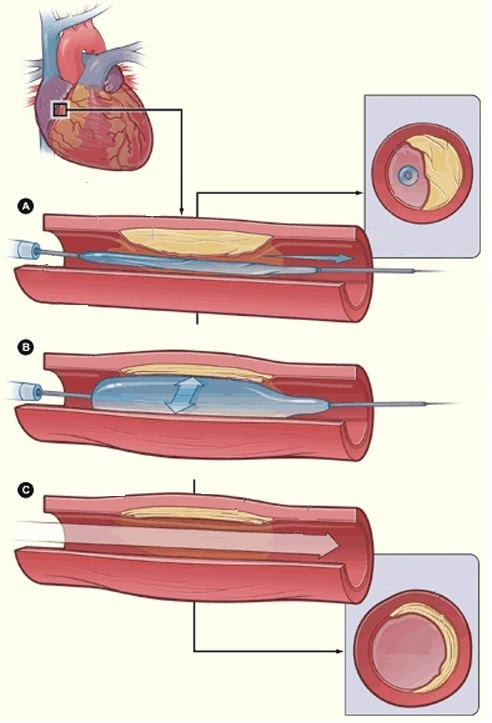
\includegraphics[scale=0.5]{./02_chaps/cap_review/figure/balloon.jpg}\\
      (a) balloon procedure
     \end{minipage}%
     \begin{minipage}{.50\linewidth}
      \centering
      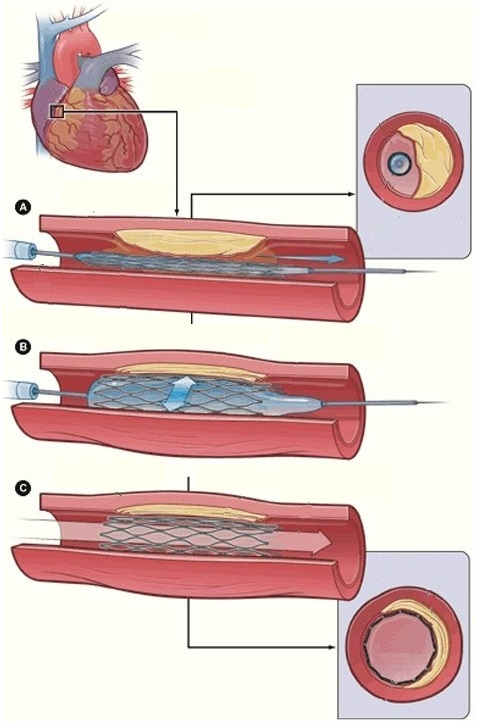
\includegraphics[scale=0.5]{./02_chaps/cap_review/figure/stent_bare.jpg}\\
      (b) stent strut procedure
     \end{minipage}\\[3mm]
     \source Source: https://medicine.umich.edu 
     \label{procedimentos PTCA}
\end{figure}

\medskip
In 2001, Hwang, Wu and Edelman \cite{hwang2001} presented a simulation of stent implantation
coated with a drug in a coronary artery. 
The simulation presented the
close relationship between drug distribution and \textit{Peclet number}
in addition to the importance of developing geometries for stents that enhance
the diffusion of the chemical substance. 
Such procedure proved to be a promising option
for the treatment of atherosclerosis and reestonosis. 
This new type of stent
would be known as \textit{drug-eluting stent}.


\medskip
In 2009, Zunino et al. \cite{zunino2009} presented a complete overview
of mathematical models and finite element numerical simulation 
applied to the  modelling of drug eluting stens and 
of their interaction with
the coronary arteries, take into account the stent expansion,
fluid dynamics around the stent and drug release. The numerical
simulation shown recirculation zones downstream 
has important consequences on the drug release process.
The smooth and concave shape of stent contours shows that
part of the drug released and accumulated in the neighborbood
of the links is transported away and may affect the arterial
walls located downstream. However, for the case analyzed,
the authors concluded that the drug released into the lumem
does not significantly contribute to the permanent drug
deposition into the arterial wall and only an small fraction of
the total amount drug stored into the stent was effectively
delivered to the artery.


\medskip
In 2014, Bozsak, Chomaz and Barakat \cite{bozsak2014} propose a computational model of transport
of the drugs \textit{paclitaxel} and \textit{sirolimus} on the artery wall. Such drugs are
frequently used in drug-eluting stents. The model takes into account the structure in
multilayer of the artery wall and these layers were modeled as porous media.
Thus, the law of \textit{Darcy} was used to simulate the flow within the layers
of the artery. The simulation showed that the choice of the type of drug used
is a crucial parameter in the creation of the drug-eluting stent
due to transport in the artery wall.


\medskip
In 2016, Bukac et al. \cite{bukac2016} present a fluid-structure
interaction between a curved coronary artery with an implanted stent,
pulsatile blood flow and heart contractions. 
An finite element numerical simulation
was performed using ALE approach and the Navier-Stokes equations for
an incompressible, viscous fluid are used to model the blood flow.
The performance of the four commercially 
available stent geometries stent struts was evaluated based on the
pathobiologic parameters responses leading to restenosis 
in the curved coronary arteries and the horizontal sinusoidal of
\textit{Cypher stent struts} performed the best in terms of theses
parameters. However, on limitation of the model used in the work 
is that it does not account for the protrusion of stent struts into the
vessel lumen. Thus, the influence of small-scale vortices around
stent struts on wall shear stress was not studied.


\medskip
Recently, Wang et al. \cite{wang2017} present the simulation
 of blood flow in a coronary artery with atherosclerosis and
 drug-eluting stent placed. Blood is approximated as a Newtonian and
 monophase fluid and the governing equations were approximated
 according to the Finite Element Method. Several axisymmetric
 geometries were presented, including a real coronary artery.
 Such geometries were used for this current work, but modified
 for a two-dimensional approach. The simulations showed that
 the proposed simplified artery with atherosclerosis model
 produced similar results of velocity, pressure and concentration
 when compared to the real artery.

\medskip
The following year, Lucena et al. \cite{lucena2018} present 
the simulation of the transport of the drug \textit{sirolimus}
 on the wall of an artery modeled as a porous and anisotropic medium.
 Dissolution in the polymeric stent lining in addition to transport
 in the artery wall in an axisymmetric domain was considered.
 The government equations were approximated according to
 the Finite Element Method. The work showed that the evolution time
 of the transport process can be efficiently controlled by
 the mass diffusivity of the polymer. It is estimated that
 about 47\% of the drug is diffused in the lumen and is lost in
 the bloodstream. The spatial distribution of the drug, however,
 is greatly influenced by blood flow and the properties of 
the artery wall. Thus, such results are susceptible to the
 patient's health conditions.

\medskip
In 2019, Gudino, Oishi and Sequeira \cite{gudino2019} presented
the influence of non-Newtonian blood flow models on drug
diffusion from a coronary drug-eluting stent. 
The Oldroyd-B, Phan-Thien-Tanner and Giesekus viscoelastic models
were used to describe the fluid dynamics of blood and the finite
element method was used for numerical simulations. The simulations
shown the hemodynamics captured by each model are more significant
in the proximal recirculation zones. The comparison between the
newtonian and non-newtonian model were performed and
the results of total stress tensor as well as the drug concentration in the artery
wall showed significant differences between the models. 


\medskip
Over the past and current decade, several drug-eluting stents
 have been developed such as: \textit{Ravel} \cite{morice2002},
 \textit{Taxus I and Taxus II} \cite{grube2003} \cite{colombo2003},
 \textit{C-Sirius} \cite{schampaert2004},
 \textit{Smart} \cite{ardissino2004} and
 more recent ones as presented in \ref{stent drug}. 
Currently, a new generation of stents has been developed
 in which the entire structure is absorbed. 
Such a generation is known as \textit{bioabsorbable stent}, 
the use of this technology is not the subject of this work.


\begin{figure}[H]
 \caption{Several models of drug-eluting stent}
  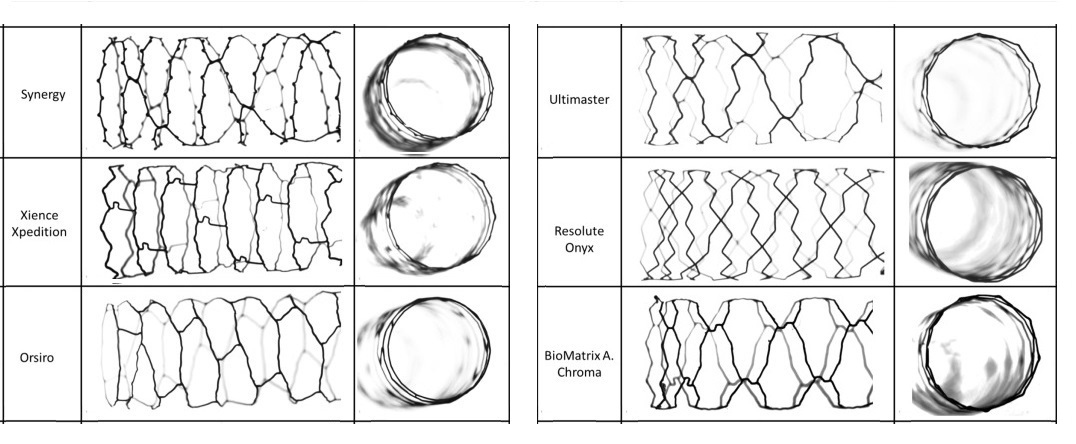
\includegraphics[scale=0.66]{./02_chaps/cap_review/figure/stent_drug.jpg}\\
 \source Source: Jaryl et al. (2016) \cite{stent2016}.
 \label{stent drug}
\end{figure}



\section{\textbf{Finite Element Method - Convection-Diffusion Equation}} 
\label{sec:secname}

The mathematical basis for the Finite Element Method begins in 1909
 with Ritz in which a continuous problem is replaced by 
a discrete problem with a finite number of degrees of freedom
 where the unknowns were approximated by the product between
 the constants to be determined and the base functions chosen
 in order to guarantee the accuracy of the result.
 This procedure is known as \textit{variational formulation}.
 Years later, Galerkin uses the Weighted Residual Method
 to determine the constants of the variational formulation
 where the same base functions were used in the weight functions.
 This procedure is known as \textit{Galerkin's formulation} and
 is widely used nowadays.

\medskip
During the 1940s, Courant (1943) \cite{courant1943} applied
 variational formulation to a domain discretized by triangular elements.
 In 1965, Zienkicwicz and Cheung \cite{zienkiewicz1965}
 show that the Weighted Residual Method has a good approximation
 of the solution and the Finite Element Method was formalized
 to solve several problems. The proposed mathematical approach
 is often used today.

\medskip
The Finite Element Method has become a very effective tool
 in the solution of several problems and it has been widely
 used in problems of the solids mechanics.
 In fluid mechanics, however, its use became possible only
 later due to the spurious oscillations that it can be seen
 when the convective term is superior to the diffusive term.
 Such oscillations are present not only in the Finite Element Method
 but were also observed in the Finite Difference Method by
 Spalding in 1972 \cite{spalding1972} where it is shown that
 the \textit{upwind} effect helped to reduce these oscillations.

\medskip
In 1976, Christie et al. \cite{christie1976} modify weight
 functions for asymmetric or quadratic functions to reduce
 spurious oscillations in one-dimensional diffusion-convection problems.
 Such modifications produced a \textit{upwind} effect on the solution.
 This procedure became known as \textit{Petrov Galerkin Formulation}.
 In the following year, Heinrich, Huyakorn and Zienkiewicz
 \cite{heinrich1977} generalize the scheme to a two-dimensional problem.
 The global matrices, however, became asymmetrical differently
 from those presented in the Galerkin scheme.

\medskip
In 1982, Brooks and Hughes \cite{brooks1982} proposed a
 new formulation that consists of modifying the weight functions
 so that the diffusion operator acts only in the flow direction.
 This procedure appears in order to eliminate the excess of
 diffusion perpendicular to the flow that
 the Petrov-Galerkin scheme presented in some cases.
 The formulation does not require the use of high-order
 weight functions and was efficient in eliminating perpendicular
 diffusion. The formulation received the name
 \textit{Streamline Upwind Petrov-Galerkin} (SUPG).


\medskip
In the same year, Pironneau \cite{pironneau1982} presented
 the Characteristic Curves Method applied to the
 Finite Element Method in solving the non-steady convection-diffusion
 and Navier-Stokes equations. Thereby, the author was able
 to derive conservative schemes of the type \textit{upwind}
 with first and second order accurate. As the matrices are symmetric,
 this scheme proved to be advantageous in solving linear
 systems compared to other \textit{upwind} schemes.
 Numerical implementation, however, requires numerical integration
 in the assembly of the vectors on the right side of the equation.
 This scheme initiates several works and is known later on as
 \textit {Characteristic Galerkin}.


\medskip
In 1984, Donea \cite{donea1984} presents an alternative for
 solving multidimensional and transient convection-diffusion
 problems. This alternative is known as the
 \textit{Taylor-Galerkin} scheme. The scheme consists of using
 the high-order terms of the Taylor expansion to reduce
 spurious oscillations. Unlike upwind schemes, in the
 Taylor-Galerkin scheme there is no need to use modified
 weight functions. The scheme is compared with the formulations
 of Galerkin and Petrov Galerkin and showed high precision and
 low numerical diffusion. Although the Taylor Galerkin and
 Characteristic Galerkin discretization procedures are distinct,
 the system of equations is identical for the convection-diffusion
 equation, where the unknowns is a scalar as mentioned by
 Lohner \cite{lohner1984}.

\medskip
Several researchers have analyzed the stability and convergencei
 of these schemes and even the implementation of more efficient
 schemes has emerged, such as the numerical simulation presented
 by Anjos et at. in 2006 \cite{anjos2006}, in which the
 \textit{semi-Lagrangean} scheme is implemented in the modeling
 of flows coupled to the transport of chemical species in
 a Finite Element approach. This scheme was widely used in
 meteorology and consists of calculating the material derivative
 along the characteristic trajectory. The discretization in time
 is done by first order backward differences while
 the discretization in space is performed according to
 the Galerkin scheme. The results showed that
 the semi-Lagrangian scheme is stable, showing no spurious
 oscillations and excessive numerical diffusion even
 for long time steps and high Reynolds and Schmidt numbers.
 Spurious oscillations in the Galerkin, SUPG and semi-Lagrangean
 schemes are compared by Silva (2011) \cite{silva2011} and
 theys are presented in \ref{spurious oscillations procedures}.

\begin{figure}[H]
     \begin{minipage}{.32\linewidth}
      \centering
      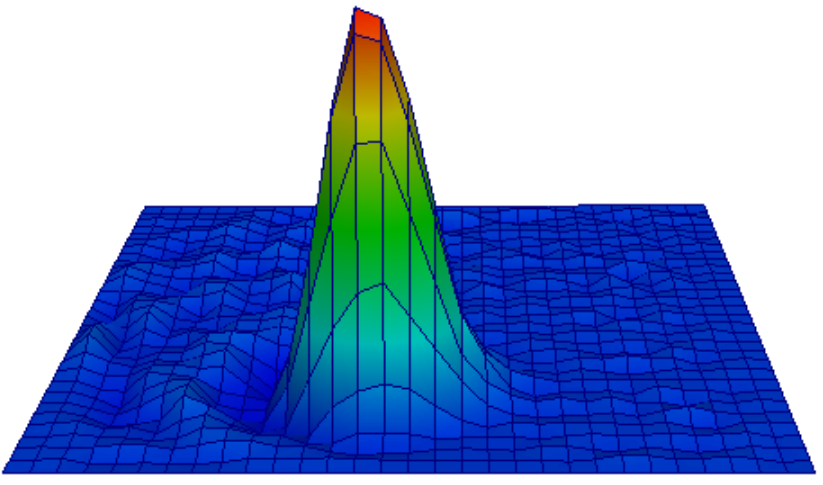
\includegraphics[scale=0.15]{./02_chaps/cap_review/figure/galerkin.png}\\
      (a)
     \end{minipage}%
     \begin{minipage}{.32\linewidth}
      \centering
      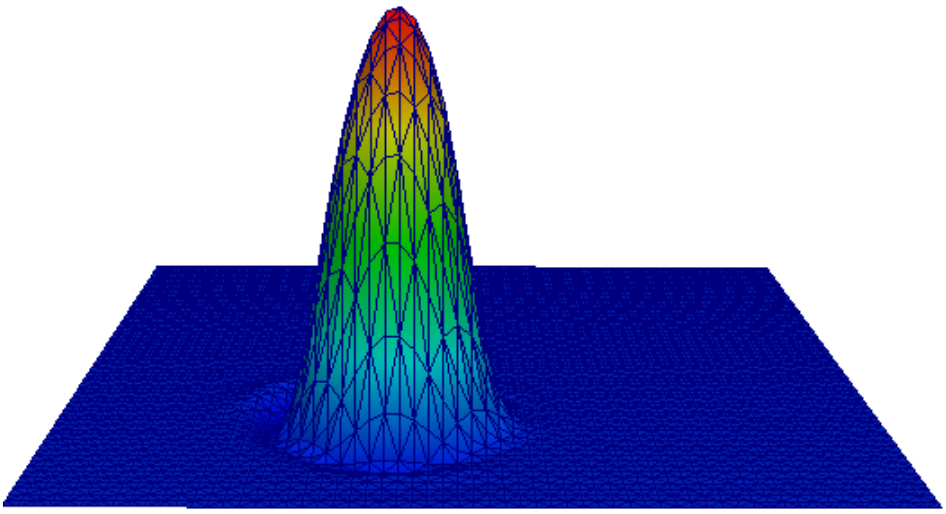
\includegraphics[scale=0.15]{./02_chaps/cap_review/figure/SUPG.png}\\
      (b)
     \end{minipage}%
     \begin{minipage}{.35\linewidth}
      \centering
      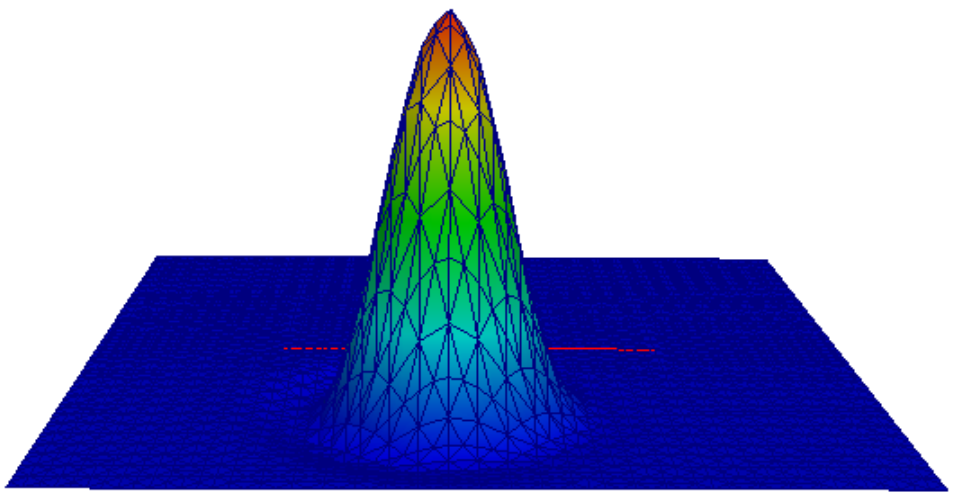
\includegraphics[scale=0.15]{./02_chaps/cap_review/figure/semilagrangian.png}\\
      (c)
     \end{minipage}%
     \medskip
     \caption{Comparison between spurious oscillations \cite{silva2011}:
              (a) Galerkin,
              (b) SUPG e 
              (c) semi-Lagrangian.}
     \label{procedimentos oscilacoes espurias}
\end{figure}



\medskip
The scheme choice to be used to reduce spurious oscillations
 is related to its advantages and disadvantages when compared
 to other schemes. In comparison to the Petrov-Galerkin and
 SUPG schemes, the Taylor-Galerkin, Characteristic and
 semi-Lagrangian schemes have the advantage of generating
 symmetric matrices facilitating computational implementation.
 Whereas, although the effectiveness of the semi-Lagrangian scheme
 is well known, it requires an efficient search algorithm for
 neighboring nodes to perform the interpolation.
 However, in Taylor-Galerkin and Characteristic Galerkin schemes,
 this need does not exist, so computational implementation becomes
 smooth. In addition, the system of linear equations generated by
 the Taylor-Galerkin scheme is similar to that generated by
 the Characteristic Galerkin scheme when the unknowns are scalar.
 Thus, the choice between these two schemes does not matter because 
 they produce similar results although the discretization process
 is different.

\medskip
All the schemes presented have satisfactory results and
they are well known in the literature.
 These schemes, therefore, made it possible to solve
 convective problems using the Finite Element Method.
 In this work, the semi-Lagragina scheme was chosen for
 the simulations.



\chapter{\textbf{GOVERNING EQUATIONS}}
\label{eqgov}

\section{\textbf{Introduction}} 
Neste trabalho, o fluido é considerado como
um meio contínuo. Isso significa que dado um elemento
de fluido infinitesimal, o mesmo é suficientemente grande
para que não haja a presença de espaços vazios em seu meio.
Dessa forma, um escoamento
pode ser modelado segundo os princípios de conservação
universal tais como:

\begin{itemize}
 \item Conservação da Massa
 \item Conservação da Quantidade de Movimento Linear
 \item Conservação de Espécie Química
\end{itemize}

Estes são os princípios que governam o escoamento
proposto neste trabalho. Na seção \ref{conservacao massa},
apresentaremos o princípio da 
conservação da massa e a \textit{equação da continuidade}
para um fluido incompressível. 
Na seção \ref{conservacao movimento}, a \textit{equação de Navier-Stokes} 
para um fluido incompressível é apresentada
segundo o princípio de conservação da
quantidade de movimento linear para um elemento de fluido.
Já na seção \ref{conservacao especie}, apresentaremos a \textit{equação de Transporte
de Espécie Química}. 
Em seguida, as equações de governo são adimensionalizadas na seção \ref{adimensionalizacao}
e a equação de Navier-Stokes é apresentada
segundo a \textit{formulação corrente-vorticidade} na seção \ref{corrente vorticidade}.


\section{\textbf{Arbitrary Lagrangian-Eulerian}} 
\label{ale}
The choice of the kinematical description of the continuum is 
extremely important for the development of a computational code, 
since it directly affects the accuracy of the numerical result. 
In the literature, two classic descriptions are commonly used, 
namely Lagrangian and Eulerian.

\medskip
The Lagrangian description is one where each computational mesh node 
moves at the same velocity as the material point, as can be seen in
\ref{ale fig}a. Thus, for each time step, we have a new computational mesh. 
The main advantage of this description is that the value of the 
computational mesh node will have the same value as the material point
 and thus, numerical diffusion will not be observed. In addition, 
the Lagrangian description makes it possible to perform 
fluid-structure interaction simulations. However, for large 
deformations, it is necessary to implement an insetion and deletion
node algorithm for computational mesh.

\medskip
The Eulerian description is the one where the computational mesh node 
remains fixed for each time step, as can be seen in \ref{ale fig}b.
Thus, the computational mesh node value will be an interpolation 
of the material point, causing the presence of numerical diffusion 
in the solution. However, the computational cost is relatively 
attractive since it is not necessary the remeshing in each time step.

\medskip
A description, however, that combines the advantages of these two 
classic descriptions as well as minimizing their disadvantages would be
most appropriate. In this context that the Arbitrary 
Lagrangian-Eulerian description (ALE) was developed. 
This description considers that the velocity field of computational 
mesh is unlike than the material point and null value, as can be seen 
in \ref{ale fig}c. In this way, it can be calculated as a 
linear combination of other velocity fields, so that we have an 
optimal relationship between numerical diffusion and mesh deformation. 
In addition, it is possible to assign several velocity values to 
specific regions of the problem in order to improve the 
accuracy of the solution.



\begin{figure}[H]
\begin{center}
\begin{tikzpicture}[scale=1.7]

 % (a) Lagrangian
 % -------------------------------------------------------------------
 % bottom line
 \draw[line width=0pt] (0,5) -- (6,5);


 % mesh motion
 \draw [line width=0pt] (0,  5) -- (0.5,6)  ;
 \draw [line width=0pt] (1,  5) -- (1.4,6)  ;
 \draw [line width=0pt] (2.7,5) -- (2.3,6);
 \draw [line width=0pt] (4,  5) -- (3.5,6)  ;
 \draw [line width=0pt] (5.1,5) -- (4.6,6);
 \draw [line width=0pt] (6,  5) -- (5.4,6)  ;

 % particle motion
 \draw [dashed,line width=0pt] (0,  5) -- (0.5,6)  ; 
 \draw [dashed,line width=0pt] (1,  5) -- (1.4,6)  ; 
 \draw [dashed,line width=0pt] (2.7,5) -- (2.3,6);   
 \draw [dashed,line width=0pt] (4,  5) -- (3.5,6)  ; 
 \draw [dashed,line width=0pt] (5.1,5) -- (4.6,6);   
 \draw [dashed,line width=0pt] (6,  5) -- (5.4,6)  ; 



 \node[square, fill=white, draw, inner sep=0pt, minimum size=9pt] at (0,5) {};
 \node[square, fill=white, draw, inner sep=0pt, minimum size=9pt] at (1,5) {};
 \node[square, fill=white, draw, inner sep=0pt, minimum size=9pt] at (2.7,5) {};
 \node[square, fill=white, draw, inner sep=0pt, minimum size=9pt] at (4,5) {};
 \node[square, fill=white, draw, inner sep=0pt, minimum size=9pt] at (5.1,5) {};
 \node[square, fill=white, draw, inner sep=0pt, minimum size=9pt] at (6,5) {};

 \node[circle, fill=black, inner sep=0pt, minimum size=5pt] at (0,5) {};
 \node[circle, fill=black, inner sep=0pt, minimum size=5pt] at (1,5) {};
 \node[circle, fill=black, inner sep=0pt, minimum size=5pt] at (2.7,5) {};
 \node[circle, fill=black, inner sep=0pt, minimum size=5pt] at (4,5) {};
 \node[circle, fill=black, inner sep=0pt, minimum size=5pt] at (5.1,5) {};
 \node[circle, fill=black, inner sep=0pt, minimum size=5pt] at (6.0,5) {};

 % top line
 \draw[line width=0pt] (0.5,6) -- (5.4,6);

 \node[square, fill=white, draw, inner sep=0pt, minimum size=9pt] at (0.5,6) {};
 \node[square, fill=white, draw, inner sep=0pt, minimum size=9pt] at (1.4,6) {};
 \node[square, fill=white, draw, inner sep=0pt, minimum size=9pt] at (2.3,6) {};
 \node[square, fill=white, draw, inner sep=0pt, minimum size=9pt] at (3.5,6) {};
 \node[square, fill=white, draw, inner sep=0pt, minimum size=9pt] at (4.6,6) {};
 \node[square, fill=white, draw, inner sep=0pt, minimum size=9pt] at (5.4,6) {};

 \node[circle, fill=black, inner sep=0pt, minimum size=5pt] at (0.5,6) {};
 \node[circle, fill=black, inner sep=0pt, minimum size=5pt] at (1.4,6) {};
 \node[circle, fill=black, inner sep=0pt, minimum size=5pt] at (2.3,6){};
 \node[circle, fill=black, inner sep=0pt, minimum size=5pt] at (3.5,6) {};
 \node[circle, fill=black, inner sep=0pt, minimum size=5pt] at (4.6,6) {};
 \node[circle, fill=black, inner sep=0pt, minimum size=5pt] at (5.4,6) {};


 % Eulerian legend 
 \draw [latexnew-latex] (-0.3,5) -- (-0.3,6);
 \node at (-0.5,5.5) {$t$};
 \node at (3,4.7) {(a)};
 % -------------------------------------------------------------------
 


 % (b) Eulerian
 % -------------------------------------------------------------------
 % bottom line
 \draw (0,2.5) -- (6,2.5);

 % mesh motion
 \draw  (0,  2.5) -- (0,  3.5)  ;
 \draw  (1,  2.5) -- (1,  3.5)  ;
 \draw  (2.7,2.5) -- (2.7,3.5)  ;
 \draw  (4,  2.5) -- (4,  3.5)  ;
 \draw  (5.1,2.5) -- (5.1,3.5)  ;
 \draw  (6,  2.5) -- (6,  3.5)  ;

 % particle motion
 \draw [dashed] (0,  2.5) -- (0.5,3.5);
 \draw [dashed] (1,  2.5) -- (1.4,3.5);
 \draw [dashed] (2.7,2.5) -- (2.3,3.5);
 \draw [dashed] (4,  2.5) -- (3.5,3.5);
 \draw [dashed] (5.1,2.5) -- (4.6,3.5);
 \draw [dashed] (6,  2.5) -- (5.4,3.5):





 \node[square, fill=white, draw, inner sep=0pt, minimum size=9pt] at (0,2.5) {};
 \node[square, fill=white, draw, inner sep=0pt, minimum size=9pt] at (1,2.5) {};
 \node[square, fill=white, draw, inner sep=0pt, minimum size=9pt] at (2.7,2.5) {};
 \node[square, fill=white, draw, inner sep=0pt, minimum size=9pt] at (4,2.5) {};
 \node[square, fill=white, draw, inner sep=0pt, minimum size=9pt] at (5.1,2.5) {};
 \node[square, fill=white, draw, inner sep=0pt, minimum size=9pt] at (6,2.5) {};

 \node[circle, fill=black, inner sep=0pt, minimum size=5pt] at (0,  2.5) {};
 \node[circle, fill=black, inner sep=0pt, minimum size=5pt] at (1,  2.5) {};
 \node[circle, fill=black, inner sep=0pt, minimum size=5pt] at (2.7,2.5) {};
 \node[circle, fill=black, inner sep=0pt, minimum size=5pt] at (4,  2.5) {};
 \node[circle, fill=black, inner sep=0pt, minimum size=5pt] at (5.1,2.5) {};
 \node[circle, fill=black, inner sep=0pt, minimum size=5pt] at (6.0,2.5) {};

 % top line
 \draw (0,3.5) -- (6,3.5);

 \node[square, fill=white, draw, inner sep=0pt, minimum size=9pt] at (0.5,3.5) {};
 \node[square, fill=white, draw, inner sep=0pt, minimum size=9pt] at (1.4,3.5) {};
 \node[square, fill=white, draw, inner sep=0pt, minimum size=9pt] at (2.3,3.5) {};
 \node[square, fill=white, draw, inner sep=0pt, minimum size=9pt] at (3.5,3.5) {};
 \node[square, fill=white, draw, inner sep=0pt, minimum size=9pt] at (4.6,3.5) {};
 \node[square, fill=white, draw, inner sep=0pt, minimum size=9pt] at (5.4,3.5) {};

 \node[circle, fill=black, inner sep=0pt, minimum size=5pt] at (0,  3.5) {};
 \node[circle, fill=black, inner sep=0pt, minimum size=5pt] at (1,  3.5) {};
 \node[circle, fill=black, inner sep=0pt, minimum size=5pt] at (2.7,3.5){};
 \node[circle, fill=black, inner sep=0pt, minimum size=5pt] at (4,  3.5) {};
 \node[circle, fill=black, inner sep=0pt, minimum size=5pt] at (5.1,3.5) {};
 \node[circle, fill=black, inner sep=0pt, minimum size=5pt] at (6.0,3.5) {};


 % Eulerian legend 
 \draw [latexnew-latex] (-0.3,2.5) -- (-0.3,3.5);
 \node at (-0.5,3) {$t$};
 \node at (3,2.2) {(b)};
 % -------------------------------------------------------------------
 


 % (c) ALE
 % -------------------------------------------------------------------
 % bottom line
 \draw (0,0) -- (6,0);

 % mesh motion
 \draw  (0,0.0) -- (0.2,1);
 \draw  (1,0.0) -- (1.1,1);
 \draw  (2.7,0.0) -- (2.8,1);
 \draw  (4,0.0) -- (3.8,1);
 \draw  (5.1,0.0) -- (4.9,1);
 \draw  (6,0.0) -- (5.8,1);

 % particle motion
 \draw [dashed] (0.0,0.0) -- (0.5,1.0);
 \draw [dashed] (1.0,0.0) -- (1.4,1.0);
 \draw [dashed] (2.7,0.0) -- (2.3,1.0);
 \draw [dashed] (4.0,0.0) -- (3.5,1.0);
 \draw [dashed] (5.1,0.0) -- (4.6,1.0);
 \draw [dashed] (6.0,0.0) -- (5.4,1.0):




 \node[square, fill=white, draw, inner sep=0pt, minimum size=9pt] at (0,0) {};
 \node[square, fill=white, draw, inner sep=0pt, minimum size=9pt] at (1,0) {};
 \node[square, fill=white, draw, inner sep=0pt, minimum size=9pt] at (2.7,0) {};
 \node[square, fill=white, draw, inner sep=0pt, minimum size=9pt] at (4,0) {};
 \node[square, fill=white, draw, inner sep=0pt, minimum size=9pt] at (5.1,0) {};
 \node[square, fill=white, draw, inner sep=0pt, minimum size=9pt] at (6,0) {};

 \node[circle, fill=black, inner sep=0pt, minimum size=5pt] at (0,0) {};
 \node[circle, fill=black, inner sep=0pt, minimum size=5pt] at (1,0) {};
 \node[circle, fill=black, inner sep=0pt, minimum size=5pt] at (2.7,0) {};
 \node[circle, fill=black, inner sep=0pt, minimum size=5pt] at (4,0) {};
 \node[circle, fill=black, inner sep=0pt, minimum size=5pt] at (5.1,0) {};
 \node[circle, fill=black, inner sep=0pt, minimum size=5pt] at (6.0,0) {};

 % top line
 \draw (0.2,1) -- (5.8,1);

 \node[square, fill=white, draw, inner sep=0pt, minimum size=9pt] at (0.5,1) {};
 \node[square, fill=white, draw, inner sep=0pt, minimum size=9pt] at (1.4,1) {};
 \node[square, fill=white, draw, inner sep=0pt, minimum size=9pt] at (2.3,1) {};
 \node[square, fill=white, draw, inner sep=0pt, minimum size=9pt] at (3.5,1) {};
 \node[square, fill=white, draw, inner sep=0pt, minimum size=9pt] at (4.6,1) {};
 \node[square, fill=white, draw, inner sep=0pt, minimum size=9pt] at (5.4,1) {};

 \node[circle, fill=black, inner sep=0pt, minimum size=5pt] at (0.2,1) {};
 \node[circle, fill=black, inner sep=0pt, minimum size=5pt] at (1.1,1) {};
 \node[circle, fill=black, inner sep=0pt, minimum size=5pt] at (2.8,1) {};
 \node[circle, fill=black, inner sep=0pt, minimum size=5pt] at (3.8,1) {};
 \node[circle, fill=black, inner sep=0pt, minimum size=5pt] at (4.9,1) {};
 \node[circle, fill=black, inner sep=0pt, minimum size=5pt] at (5.8,1) {};


 % ALE legend 
 \draw [latexnew-latex] (-0.3,0) -- (-0.3,1);
 \node at (-0.5,0.5) {$t$};
 \node at (3,-0.3) {(c)};
 

 % picture legend
 %\node[square, draw, inner sep=0pt, minimum size=8pt] at (0.5,-0.7);
 %\node[circle, fill=black, inner sep=0pt, minimum size=4pt] at (0.5,-1.2);
 %\draw [dotted] (3.5,-0.7) -- (4.08,-0.7);
 %\draw [dashed] (3.5,-1.2) -- (4.1,-1.2);

 %\node at (1.7,-0.7) {\tiny material point};
 %\node at (1.2,-1.2) {\tiny node};
 %\node at (5.2,-0.7) {\tiny particle motion};
 %\node at (5.1,-1.2) {\tiny mesh motion};
 % -------------------------------------------------------------------


\end{tikzpicture}
\end{center}
\caption{One-dimensional examples of the (a) Lagrangian description, (b) Eulerian description and (c) ALE description, where the white square is the material point, the black point is the mesh node, the dashed line is the characteristic trajectory and the continuous line is mesh nodes trajectory.}
\label{ale fig}
\end{figure}



\medskip
The ALE description was first implemented in the finite difference
 method, as presented by Hirt et al. (1974) \cite{hirt1974} 
and was subsequently adopted in the finite elements context, 
as presented by Donea (1982) \cite{donea1982}. In this description, 
the referential domain that describes the computational mesh moving 
is different from the material domain and the spatial domain, 
as shown in the \ref{referential domain}. 
However, it is possible to correlate these 
frameworks. For instance, if the $\Phi$ operator is equal to the 
identity matrix (\textbf{I}), then the referential and material domain 
is the same and, subsequently, the node velocity of the 
computational mesh 
is equivalent to the material points velocity (Lagrangian description). 
But, if the $\Psi$ operator is equal to \textbf{I}, the computational mesh
velocity is equivalent to null value and then the Eulerian description is
obtained. For more details, it is possible to consult the works 
of Donea (2004) \cite{donea2004} and Hughes (1981) \cite{hughes1981}.

\begin{figure}[H]
\begin{center}
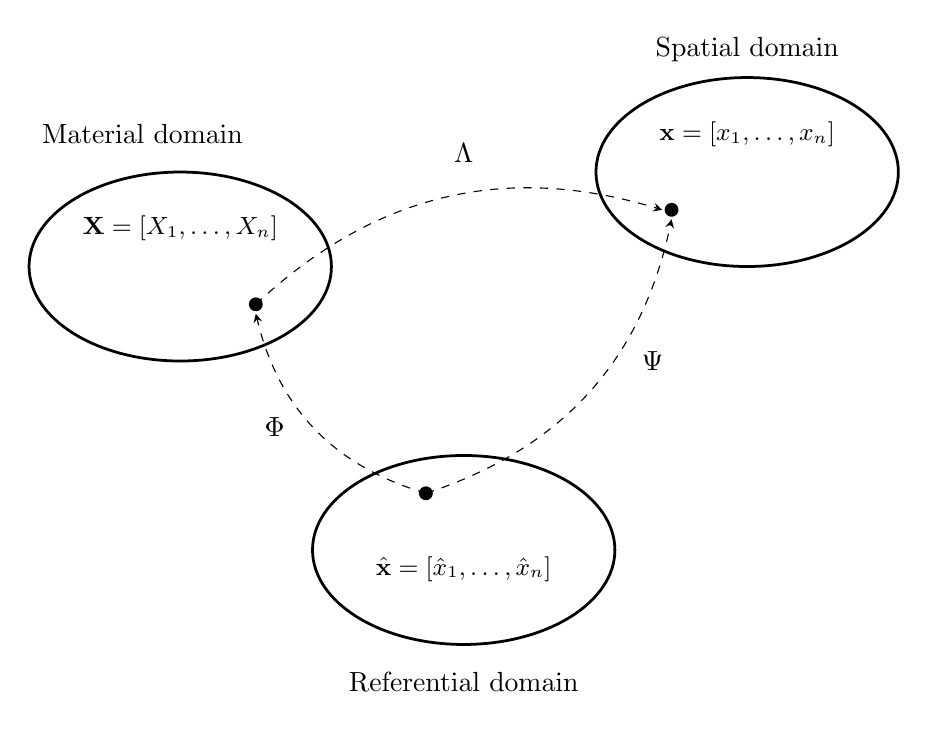
\begin{tikzpicture}[scale=2.4]
 \draw[line width=1pt] (-1.5,0) ellipse(0.8cm and 0.5cm);
 \draw[line width=1pt] (1.5,0.5) ellipse(0.8cm and 0.5cm);
 \draw[line width=1pt] (0,-1.5) ellipse(0.8cm and 0.5cm);
 
 \node[circle, fill=black, inner sep=0pt, minimum size=5pt] at (-0.2,-1.2) {};
 \node[circle, fill=black, inner sep=0pt, minimum size=5pt] at (-1.1,-0.2) {};
 \node[circle, fill=black, inner sep=0pt, minimum size=5pt] at (1.1,0.3) {};

 \node at (0.0,-1.6) {\small $\hat{\textbf{x}}=[\hat{x}_{1},\ldots,\hat{x}_{n}]$};
 \node at (-1.5,0.2) {\small $\textbf{X}=[X_{1},\ldots,X_{n}]$};
 \node at (1.5,0.7) {\small $\textbf{x}=[x_{1},\ldots,x_{n}]$};

 \draw[dashed,-stealth] (-0.2,-1.2) to[bend left=30]  (-1.10,-0.25);
 \draw[dashed,-stealth] (-0.2,-1.2) to[bend right=30] (1.10, 0.25);
 \draw[dashed,-stealth] (-1.1,-0.2) to[bend left=30]  (1.05, 0.30);

 \node at (-1.0,-0.85) {$\Phi$};
 \node at (1.0,-0.50) {$\Psi$};
 \node at (0.0,0.6) {$\Lambda$};

 \node at (-1.7,0.7) {Material domain};
 \node at (1.5,1.15) {Spatial domain};
 \node at (0.0,-2.2) {Referential domain};



\end{tikzpicture}
\end{center}
\caption{
Material, Spatial and Referential domains for the Artibratiry Lagrangian-Eulerian description.
}
\label{referential domain}
\end{figure}






%\medskip
%Therefore, the material point velocity that travels from 
%the material domain to the spatial domain may be obtained 
%according to the X operator:
%
%equation 4 (donea2004)
%
%\medskip
%\noindent
%Whereas, the computational mesh velocity that travels from the 
%referential domain to the spatial domain may be obtained according 
%to the Y operator:
%
%equation 7 (donea2004)
%
%\medskip
%\noindent
%Finally, we can describe the transport of any property f in 
%the spatial domain according to the ALE description as:
%
%equation 3.3 (phd2012)


\section{\textbf{Mass Conservation}} 
\label{conservacao massa}
As presented by Batchelor (1967) \cite{batchelor1967},
 the principle of mass conservation without source term
 establishes that:


\medskip
\begin{center}
\textarray{Mass accumulation rate\\
           on control volume}
           $= -$ 
\textarray{Mass flux crossing\\ 
           the boundary}
\end{center}

\noindent Mathematically, the mass accumulation rate within on volume
 can be represented by:

\begin{equation} \label{massa 1} 
 \int_{V} \frac{\partial}{\partial t} dm
\end{equation}


\noindent where the infinitesimal mass $dm$ is defined
 as $dm = \rho dV$. Replacing it in Eq. \ref{massa 1}
 and considering that the control volume does not vary over time,
 we have:

\begin{equation}
 \int_{V} \frac{\partial}{\partial t} dm
 =
 \int_{V} \frac{\partial}{\partial t} \big( \rho dV \big)
 = 
 \int_{V} \frac{\partial \rho}{\partial t} dV
 +
 \int_{V} \rho \frac{\partial dV}{\partial t}
 = 
 \int_{V} \frac{\partial \rho}{\partial t} dV
\end{equation}

\medskip
\noindent The mass flux crossing boundary can be mathematically represented by:


\begin{equation}  
 \oint_{S} \rho \left(\textbf{v} - \hat{\textbf{v}}\right) \cdot \textbf{n} dA
\end{equation}

\medskip
\noindent Thereby, according to mass conservation theorem:

\begin{equation}
 \int_{V} \frac{\partial \rho}{\partial t} dV
 = - 
 \oint_{S} \rho \left(\textbf{v} - \hat{\textbf{v}}\right) \cdot \textbf{n} dA
\end{equation}

\medskip
\noindent Applying the \textit{Gauss theorem} on surface integral:

\begin{equation}
 \int_{V} \frac{\partial \rho}{\partial t} dV
 = - 
 \int_{V} \nabla \cdot \left[ \rho \left(\textbf{v} - \hat{\textbf{v}}\right) \right] dV
\end{equation}

\medskip
\noindent
that is:

\begin{equation} \label{massa 2}
 \int_{V} \left[ \frac{\partial \rho}{\partial t}
 + 
 \nabla \cdot 
\left[ \rho \left(\textbf{v} - \hat{\textbf{v}}\right) \right] 
\right] dV 
 = 0 
\end{equation}

\medskip
\noindent 
Whereas the $dV \neq 0$,
the Eq. \ref{massa 2} can be presented as:

\begin{equation} \label{continuity equation}
 \frac{\partial \rho}{\partial t}
 + 
 \nabla \cdot 
\left[ \rho \left(\textbf{v} - \hat{\textbf{v}}\right) \right] 
 = 0 
\end{equation}

\medskip
\noindent 
where $\rho$ is density, $\textbf{v}$ is material velocity
 whose components are $\textbf{v} = \left[u,v\right]$,
$\hat{\textbf{v}}$ is mesh velocity,
$\nabla$ is Del operator whose components are 
$\nabla = \left[ \partial/\partial x, \partial / \partial y \right]$,
$x$ and $y$ are coordinates components and
$t$ is time.
The Eq. \ref{continuity equation} is known
as \textit{Continuity Equation} 
for Arbitrary Lagrangian-Eulerian description \cite{donea1982}.
Developing the equation, we have:

\begin{equation}
 \frac{\partial \rho}{\partial t}
 +
 \left(\textbf{v} - \hat{\textbf{v}}\right) \cdot \nabla \rho
 +
 \rho \nabla \cdot \textbf{v}
 = 0
\end{equation}

\medskip
According to fluid incompressible assumption,
the density does not depende on time and on coordinates.
Therefore, the 
$\partial \rho / \partial t$ e $\nabla \rho$ derivatives are 
null values.
Thus, the mass conservation is reduced to:

\begin{equation} \label{massa 3}
 \rho \nabla \cdot \textbf{v}
 = 0 
\end{equation}

\medskip
\noindent that is:

\begin{equation} \label{incompressible continuity equation}
 \nabla \cdot \textbf{v}
 = 0 
\end{equation}

\medskip
\noindent This equation is the \textit{continuity equation} for an incompressible flow.


\newpage





\section{\textbf{Linear Momentum Conservation}} 
\label{conservacao movimento}
The same concept of mass conservation is applied to the
linear momentum conservation. Therefore, the principle
of linear momentum conservation establishes that:

\medskip
\begin{center}
\textarray{Linear momentum\\
           accumulation rate\\ 
           on control volume}
           $= -$ 
\textarray{Linear momentum\\
           flux crossing\\
           the boundary}
           $+$ 
\textarray{The resultant of \\
           body force and \\ 
           surface force}
\end{center}

\medskip
Mathematically, linear momentum accumulation rate on control volume
can be presented to represented by:

\begin{equation} \label{qml 1} 
 \int_{V} \frac{\partial}{\partial t} \big( \rho \textbf{v} \big) dV
\end{equation}

\medskip
The linear momentum flux crossing the boundary
can be represented mathematically by:

\begin{equation}  
 \oint_{S} \rho \textbf{v} \textbf{v} \cdot \textbf{n} dA
\end{equation}

\medskip
The resultant force is consists of surface force and body force.
The surface force can be represented by:

\begin{equation}  
 \oint_{S} \sigma \cdot \textbf{n} dA
\end{equation}

\medskip
\noindent
where $\sigma$ is the stress tensor. 
Whereas, the body is represend by:

\begin{equation} 
 \int_{V} \rho \textbf{g} dV
\end{equation}

\medskip
\noindent
where $\textbf{g}$ is gravity vector.
Thereby, according to principle of linear momentum conservation:

\begin{equation}
 \int_{V} \frac{\partial}{\partial t} \big( \rho \textbf{v} \big) dV
 = - 
 \oint_{S} \rho \textbf{v} \textbf{v} \cdot \textbf{n} dA
 +
 \oint_{S} \sigma \cdot \textbf{n} dA
 +
 \int_{V} \rho \textbf{g} dV
\end{equation}

\medskip
\noindent
Applying the \textit{Gauss Theorem} on surface integrals:

\begin{equation}
 \int_{V} \frac{\partial}{\partial t} \big( \rho \textbf{v} \big) dV
 = - 
 \int_{V} \nabla \cdot \big( \rho \textbf{v} \textbf{v} \big) dV
 +
 \int_{V} \nabla \cdot \sigma dV
 +
 \int_{V} \rho \textbf{g} dV
\end{equation}

\medskip
\noindent
that is:

\begin{equation} \label{qm 2}
 \int_{V} \Bigg[ \frac{\partial}{\partial t} \big( \rho \textbf{v} \big)
 + 
 \nabla \cdot \big( \rho \textbf{v} \textbf{v} \big)
 -
 \nabla \cdot \sigma
 -
 \rho \textbf{g} \Bigg] dV = 0
\end{equation}



\medskip
\noindent
Whereas the $dV \neq 0$,
the Eq. \ref{qm 2} can be presented as:



\begin{equation}
 \frac{\partial}{\partial t} \big( \rho \textbf{v} \big)
 + 
 \nabla \cdot \big( \rho \textbf{v} \textbf{v} \big)
 -
 \nabla \cdot \sigma
 -
 \rho \textbf{g} = 0
\end{equation}


\medskip
\noindent
that is:

\begin{equation}
 \frac{\partial}{\partial t} \big( \rho \textbf{v} \big) 
 +
 \nabla \cdot \big( \rho \textbf{v} \textbf{v} \big)
 =
 \nabla \cdot \sigma
 +
 \rho \textbf{g}
\end{equation}

\medskip
\noindent
Developing the left hand side of equation, we have:

\begin{equation}
 \rho \frac{\partial \textbf{v}}{\partial t}
 +
 \textbf{v} \frac{\partial \rho}{\partial t}
 +
 \rho \textbf{v} \cdot \nabla \textbf{v}
 + 
 \textbf{v} \cdot \nabla \big( \rho \textbf{v} \big)
 =
 \rho \Bigg[ \frac{\partial \textbf{v}}{\partial t} + \textbf{v} \cdot \nabla \textbf{v} \Bigg]
 +
 \textbf{v} \Bigg[ \frac{\partial \rho}{\partial t} + \nabla \big( \rho \textbf{v} \big) \Bigg]
\end{equation}

\newpage
The last term of above equation is null because
 the \textit{continuity equation} (Eq. \ref{continuity equation}).
Thus, the linear momentum equation can be rewritten as:

\begin{equation} \label{qm 3}
 \rho \Bigg[ \frac{\partial \textbf{v}}{\partial t} + \textbf{v} \cdot \nabla \textbf{v} \Bigg]
 =
 \nabla \cdot \sigma
 +
 \rho \textbf{g}
\end{equation}

\medskip
\noindent
The stress tensor $\sigma$ can be split into
two tensors:

\begin{equation}
 \sigma = -p \textbf{I} + \tau
\end{equation}

\medskip
\noindent
where, $p$ is pressure field, \textbf{I} is the identity matrix and
$\tau$ id deviatoric stress. 
Replacing them in Eq. \ref{qm 3}, we have:

\begin{equation}
 \rho \Bigg[ \frac{\partial \textbf{v}}{\partial t} + \textbf{v} \cdot \nabla \textbf{v} \Bigg]
 =
 \nabla \cdot \big[ -p \textbf{I} + \tau \big]
 +
 \rho \textbf{g}
\end{equation}

\medskip
\noindent
that is:

\begin{equation} \label{qm 4}
 \rho \Bigg[ \frac{\partial \textbf{v}}{\partial t} + \textbf{v} \cdot \nabla \textbf{v} \Bigg]
 =
 -
 \nabla p
 +
 \nabla \cdot \tau
 +
 \rho \textbf{g}
\end{equation}

\medskip
The deviatoric stress $\tau$ depends on strain tensor rate and
we can define it relating to medium physical properties.
Whereas a homogeneous, isotropic fluid and the deviatoric stress
as a continuous and linear function of velocity gradient,
we have:

\begin{equation}
 \tau = \mu \big[ \nabla \textbf{v} + \big( \nabla \textbf{v} \big)^{T} \big]
      + \lambda \textbf{I} \nabla \cdot \textbf{v}
\end{equation}

\medskip
\noindent
where $\mu$ is dynamic viscosity of fluid,
$\lambda$ is known as the second viscosity coefficient and
\textbf{I} is identidy matrix.
Replacing them in Eq. \ref{qm 4}, we have:



\begin{equation} 
 \rho \Bigg[ \frac{\partial \textbf{v}}{\partial t} + \textbf{v} \cdot \nabla \textbf{v} \Bigg]
 =
 -
 \nabla p
 +
 \nabla \cdot \big[ 
 \mu \big[ \nabla \textbf{v} + \big( \nabla \textbf{v} \big)^{T} \big]
 + \lambda \textbf{I} \nabla \cdot \textbf{v}
 \big]
 +
 \rho \textbf{g}
\end{equation}


\medskip
\noindent
that is:

\begin{equation} 
 \rho \Bigg[ \frac{\partial \textbf{v}}{\partial t} + \textbf{v} \cdot \nabla \textbf{v} \Bigg]
 =
 -
 \nabla p
 +
 \nabla \cdot \big[ \mu \big[ \nabla \textbf{v} + \big( \nabla \textbf{v} \big)^{T} \big] \big]
 + 
 \nabla \cdot \big[ \lambda \textbf{I} \nabla \cdot \textbf{v} \big]
 +
 \rho \textbf{g}
\end{equation}


\medskip
\noindent
Whereas the dynamic viscosity $\mu$ does not depends on coordinates,
we have:

\begin{equation} 
 \rho \Bigg[ \frac{\partial \textbf{v}}{\partial t} + \textbf{v} \cdot \nabla \textbf{v} \Bigg]
 =
 -
 \nabla p
 +
 \mu \big[ \nabla \cdot \nabla \textbf{v} + \nabla \cdot \big( \nabla \textbf{v} \big)^{T} \big]
 +
 \nabla \cdot \big[ \lambda \textbf{I} \nabla \cdot \textbf{v} \big]
 +
 \rho \textbf{g}
\end{equation}

\medskip
\noindent
that is:

\begin{equation} 
 \rho \Bigg[ \frac{\partial \textbf{v}}{\partial t} + \textbf{v} \cdot \nabla \textbf{v} \Bigg]
 =
 -
 \nabla p
 +
 \mu \big[ \nabla^{2} \textbf{v} + \nabla \big( \nabla \cdot \textbf{v} \big) \big]
 +
 \nabla \cdot \big[ \lambda \textbf{I} \nabla \cdot \textbf{v} \big]
 +
 \rho \textbf{g}
\end{equation}

\medskip
\noindent
According to Eq. \ref{incompressible continuity equation}, we have:

\begin{equation} \label{navier-stokes}
 \frac{\partial \textbf{v}}{\partial t} + \textbf{v} \cdot \nabla \textbf{v}
 =
 -
 \frac{1}{\rho} \nabla p
 +
 \nu \nabla^{2} \textbf{v}
 +
 \textbf{g}
\end{equation}

\medskip
\noindent
where $\nu$ is the kinematic viscosity of fluid.
 The Eq. \ref{navier-stokes} is known as
\textit{Navier-Stokes Equation} and is valid for a
homogeneous, isotropic, incompressible fluid
and with viscosity that it does not depends on coordinates.

\newpage


\section{\textbf{Species Transport Conservation}} 
\label{conservacao especie}
Similarly to the previous sections, 
the species transport conservation
for a region with arbitrary motion is:


\begin{equation}
 \int_{V} \frac{\partial e}{\partial t} dV
 = 
 - 
 \oint_{S} e \textbf{c} \cdot \textbf{n} dA
 +
 \oint_{S} D \nabla e \cdot \textbf{n} dA
 +
 \int_{V} \overset{.}{R} dV
\end{equation}

\medskip
\noindent
where $D$ is the mass diffusivity and 
$\overset{.}{R}$ is the chemical species source rate.
Applying the \textit{Gauss Theorem} on surface integrals:

\begin{equation}
 \int_{V} \frac{\partial e}{\partial t} dV
 = 
 - 
 \int_{V} \nabla \cdot \big( e \textbf{c} \big) dV
 +
 \int_{V} \nabla \cdot \big( D \nabla e \big) dV
 +
 \int_{V} \overset{.}{R} dV
\end{equation}

\medskip
\noindent
that is:

\begin{equation} \label{esp 2}
 \int_{V} \Bigg[ \frac{\partial e}{\partial t}
 + 
 \nabla \cdot \big( e \textbf{c} \big)
 -
 \nabla \cdot \big( D \nabla e \big)
 -
 \overset{.}{R} \Bigg] dV = 0
\end{equation}



\medskip
\noindent
In view of the $dV \neq 0$,
the Eq. \ref{esp 2} can be represented by:

\begin{equation}
 \frac{\partial e}{\partial t}
 + 
 \nabla \cdot \big( e \textbf{c} \big)
 -
 \nabla \cdot \big( D \nabla e \big)
 -
 \overset{.}{R} = 0
\end{equation}



\medskip
\noindent
that is:

\begin{equation}
 \frac{\partial e}{\partial t}
 +
 \nabla \cdot \big( e \textbf{c} \big)
 =
 \nabla \cdot \big( D \nabla e \big)
 +
 \overset{.}{R}
\end{equation}

\medskip
\noindent
Developing the left hand side of equation, we have:

\begin{equation}
 \frac{\partial e}{\partial t}
 +
 \textbf{v} \cdot \nabla e
 + 
 e \nabla \cdot \textbf{c}
 =
 \nabla \cdot \big( D \nabla e \big)
 +
 \overset{.}{R}
\end{equation}

\medskip
The last term of above equation is null because the
fluid incompressibility assumption
(Eq. \ref{incompressible continuity equation}),
thus:

\begin{equation}
 \frac{\partial e}{\partial t}
 +
 \textbf{c} \cdot \nabla e
 =
 \nabla \cdot \big( D \nabla e \big)
 +
 \overset{.}{R}
\end{equation}

\medskip
Taking into consideration that the mass diffusiviy
is constant and without chemical species
generation,
the species transport equation can rewritten as:

\begin{equation} \label{chemical species}
 \frac{\partial e}{\partial t}
 +
 \textbf{c} \cdot \nabla e
 =
 D \nabla^{2} e
\end{equation}

\medskip
The Eq. \ref{chemical species} is known as
\textit{Species Transport Equation}
for an incompressible fluid, with constant mass diffusivity
and without chemical species generation for the
Arbitrary Lagrangian-Eulerian description.


\section{\textbf{Non-dimensionalization}} 
\label{adimensionalizacao}
In this section, the non-dimensional form
of continuity, Navier-Stokes and
species transport equations are shown.
The non-dimensionalization helps to understand 
which terms of the equation influence most during 
a given simulation in addition to allowing experiments 
with small scale models 
The following parameters was used in non-dimensionalization:

\begin{equation}
 \begin{aligned}
  p & = \rho_{0} U^{2} p^{*} \\[10pt]
 \textbf{v} & = U \textbf{v}^{*} \\
 \end{aligned}
 \qquad
 \begin{aligned}
 e & = ( e_{s} - e_{0} ) e^{*} + e_{0}\\[10pt]
 \textbf{g} & = g_{0} \textbf{g}^{*} \\
 \end{aligned}
 \qquad
 \begin{aligned}
 \nu & = \nu_{0} \nu^{*} \\[10pt]
 \rho & = \rho_{0} \rho^{*} \\
 \end{aligned}
 \qquad
 \begin{aligned}
 D & = D_{0} D^{*} \\[5pt]
 \nabla & = \frac{1}{L} \nabla^{*} \\
 \end{aligned}
 \qquad
 \begin{aligned}
 x & = L x^{*} \\[5pt]
 t & = \frac{L}{U} t^{*} \\
 \end{aligned}
 \nonumber
\end{equation}


\medskip
\noindent
where the asterisk identify the non-dimensional unknowns.
Replacing the above parameters in Eq. \ref{incompressible
continuity equation}, we have:

\begin{equation}
 \frac{U}{L} \nabla^{*} \cdot \textbf{v}^{*} = 0
\end{equation}

\medskip
\noindent
Multiplying both sides by $U/L$:

\begin{equation} \label{continuidade adimensional 1}
 \nabla^{*} \cdot \textbf{v}^{*} = 0
\end{equation}

\medskip
\noindent
A similar procedure is performed in
Eq. \ref{navier-stokes}, that is:

\begin{equation}
 \frac{U^{2}}{L} \frac{\partial \textbf{v$^{*}$}}{\partial t^{*}} 
 + 
 \frac{U^{2}}{L} \textbf{c$^{*}$} \cdot \nabla^{*} \textbf{v$^{*}$}
 =
 -
 \frac{U^{2}}{L} \frac{1}{\rho^{*}} \nabla^{*} p^{*}
 +
 \frac{\nu_{0} U}{L^{2}} \nu^{*} \nabla^{*2} \textbf{v$^{*}$}
 +
 g_{0} \textbf{g$^{*}$}
\end{equation}

\medskip
\noindent
Multiplying both sides by $L/U^{2}$:

\begin{equation} \label{navier-stokes adimensional 2}
 \frac{\partial \textbf{v$^{*}$}}{\partial t^{*}} 
 + 
 \textbf{c$^{*}$} \cdot \nabla^{*} \textbf{v$^{*}$}
 =
 -
 \frac{1}{\rho^{*}} \nabla^{*} p^{*}
 +
 \frac{\nu_{0}}{UL} \nu^{*} \nabla^{*2} \textbf{v$^{*}$}
 +
 \frac{g_{0}L}{U^{2}} \textbf{g$^{*}$}
\end{equation}

\medskip
\noindent
that is:

\begin{equation} \label{navier-stokes adimensional 1}
 \frac{\partial \textbf{v$^{*}$}}{\partial t^{*}} 
 + 
 \textbf{c$^{*}$} \cdot \nabla^{*} \textbf{v$^{*}$}
 =
 -
 \nabla^{*} p^{*}
 +
 \frac{\nu_{0}}{UL} \nabla^{*2} \textbf{v$^{*}$}
 +
 \frac{g_{0}L}{U^{2}} \textbf{g$^{*}$}
\end{equation}

\medskip
\noindent
In the Eq. \ref{chemical species}, a similar procedure is performed:

\begin{equation}
 (e_{s}-e_{0}) \frac{U}{L} \frac{\partial e^{*}}{\partial t^{*}}
 +
 (e_{s}-e_{0}) \frac{U}{L} \textbf{c$^{*}$} \cdot \nabla^{*} e^{*}
 =
 (e_{s}-e_{0}) \frac{D_{0}}{L^{2}} D^{*} \nabla^{*2} e^{*}
\end{equation}

\medskip
\noindent
Multiplying both sides by $L/U(e_{s}-e_{0})$, we have:

\begin{equation} \label{especie quimica adimensional 2}
 \frac{\partial e^{*}}{\partial t^{*}}
 +
 \textbf{c$^{*}$} \cdot \nabla^{*} e^{*}
 =
 \frac{D_{0}}{UL} D^{*} \nabla^{*2} e^{*}
\end{equation}

\medskip
\noindent
that is

\begin{equation} \label{especie quimica adimensional 1}
 \frac{\partial e^{*}}{\partial t^{*}}
 +
 \textbf{c$^{*}$} \cdot \nabla^{*} e^{*}
 =
 \frac{D_{0}}{UL} \nabla^{*2} e^{*}
\end{equation}

\noindent
where, important non-dimensional groups are found in
Eqs. \ref{continuidade adimensional 1}, \ref{navier-stokes adimensional 1}
and \ref{especie quimica adimensional 1}, such that:
\item \textbf{Reynolds Number} ($Re$),
\textbf{Froude number} ($Fr$) and
\textbf{Mass Péclet number} ($Pe_{m}$).
The $Pe_{m}$ number is often
 shown as the product of
 the \textit{Reynolds number} and the \textit{Schmidt number} $Sc$.
Replacing these non-dimensional groups in Eqs.
\ref{continuidade adimensional 1}, \ref{navier-stokes adimensional 1}
and \ref{especie quimica adimensional 1} and
removing the asterisk, we have:

\begin{equation} \label{continuidade adimensional}
 \nabla \cdot \textbf{v} = 0
\end{equation}

\begin{equation} \label{navier-stokes adimensional}
 \frac{\partial \textbf{v}}{\partial t} 
 + 
 \textbf{c} \cdot \nabla \textbf{v}
 =
 -
 \nabla p
 +
 \frac{1}{Re} \nabla^{2} \textbf{v}
 +
 \frac{1}{Fr^{2}} \textbf{g}
\end{equation}

\begin{equation} \label{especie quimica adimensional}
 \frac{\partial e}{\partial t}
 +
 \textbf{c} \cdot \nabla e
 =
 \frac{1}{ReSc} \nabla^{2} e
\end{equation}

\medskip
The Eqs.
\ref{continuidade adimensional}, 
\ref{navier-stokes adimensional} e 
\ref{especie quimica adimensional}
are, respectively, non-dimensional form of Continuity,
Navier-Stokes and Species Transport equations
for a newtonian and incompressble flow in an
Arbritary Lagrangian-Eulerian description.



\section{\textbf{Vorticity-Streamfunction Formulation}} 
\label{corrente vorticidade}
The Navier-Stokes equation has a strong coupling between
 the pressure field and the velocity field.
 This coupling makes it difficult to implement this
 equation computationally. The Decoupling of pressure
 and velocity fields is possible by using the
 \textit{Vorticity-Streamfunction Formulation}.
 For this, we will replace in the equation
 \ref{navier-stokes adimensional} the following vector identity:

\begin{equation}
 \textbf{c} \cdot \nabla \textbf{v}
 = 
 \nabla \left( \textbf{c} \cdot \textbf{v} \right)
 - 
 \textbf{c} \times \nabla \times \textbf{v}
\end{equation}

\medskip
\noindent
Therefore:

\begin{equation}
 \frac{\partial \textbf{v}}{\partial t} 
 + 
 \nabla \left( \textbf{c} \cdot \textbf{v} \right)
 - 
 \textbf{c} \times \nabla \times \textbf{v}
 =
 -
 \nabla p
 +
 \frac{1}{Re} \nabla^{2} \textbf{v}
 +
 \frac{1}{Fr^{2}} \textbf{g}
\end{equation}

\medskip
\noindent
Computing the curl on both sides of the above equation:

\begin{equation}
 \nabla \times \frac{\partial \textbf{v}}{\partial t} 
 + 
 \nabla \times \nabla \left( \textbf{c} \cdot \textbf{v} \right)
 - 
 \nabla \times \textbf{c} \times \nabla \times \textbf{v}
 =
 -
 \nabla \times \nabla p
 +
 \frac{1}{Re} \nabla \times \nabla^{2} \textbf{v}
 +
 \frac{1}{Fr^{2}} \nabla \times \textbf{g}
\end{equation}

\medskip
\noindent
that is:

\begin{equation}
 \frac{\partial}{\partial t} \big[ \nabla \times \textbf{v} \big]
 + 
 \nabla \times \nabla \left( \textbf{c} \cdot \textbf{v} \right)
 - 
 \nabla \times \big[ \textbf{c} \times \nabla \times \textbf{v} \big]
 =
 -
 \nabla \times \nabla p
 +
 \frac{1}{Re} \nabla^{2} \big[ \nabla \times \textbf{v} \big]
 +
 \frac{1}{Fr^{2}} \nabla \times \textbf{g}
\end{equation}

\medskip
The terms that contain the gradient operator cancel
 each other out, since the curl of gradient of a scalar is zero.
 The last term is also null because the derivatives of a constant,
 as in the case of \textbf{g}, are equal to zero. Thus, we have:

\begin{equation}
 \frac{\partial}{\partial t} \big[ \nabla \times \textbf{v} \big]
 - 
 \nabla \times \big[ \textbf{c} \times \nabla \times \textbf{v} \big]
 =
 \frac{1}{Re} \nabla^{2} \big[ \nabla \times \textbf{v} \big]
\end{equation}

\medskip
\noindent
The vector $\nabla \times \textbf{v}$ is known as
\textit{vorticity} ($w$).
Therby, the equation can be represented by:

\begin{equation} \label{vort 1}
 \frac{\partial w}{\partial t}
 - 
 \nabla \times \big[ \textbf{c} \times w \big]
 =
 \frac{1}{Re} \nabla^{2} w
\end{equation}

\medskip
\noindent
The second term of left side in 
Eq. \ref{vort 1}
can be replaced by following vectorial identity:


\begin{equation}
 \nabla \times \big[ \textbf{c} \times w \big]
 =
 -
 \textbf{c} \cdot \nabla w
 +
 w \cdot \nabla \textbf{c}
\end{equation}

\medskip
\noindent
Thus the Eq. \ref{vort 1} will be:

\begin{equation} \label{vort 2}
 \frac{\partial w}{\partial t}
 +
 \textbf{c} \cdot \nabla w
 - 
 w \cdot \nabla \textbf{c}
 =
 \frac{1}{Re} \nabla^{2} w
\end{equation}

\medskip
For two-dimensional flows, as in the case of this work,
 the vorticity is perpendicular to the velocity vector.
 Thus, the product $w \cdot \nabla \textbf{c}$ will be canceled
 as presented by Pontes and Mangiavacchi (2016) \cite{pontes2016}.
 Therefore:

\begin{equation} \label{equacao vorticidade}
 \frac{\partial w}{\partial t}
 +
 \textbf{c} \cdot \nabla w
 =
 \frac{1}{Re} \nabla^{2} w
\end{equation}

\medskip
The Eq. \ref{equacao vorticidade} is known as
 \textit{vorticity equation} for two-dimensional flows of
 a Newtonian and incompressible fluid in an Arbritary
 Lagragian-Eulerian description. For a steady and 
 two-dimensional flow of incompressible fluid,
 the velocity can be calculated from the volumetric flux.
 Thereby, the velocity is replaced by a scalar.
 Such a scalar is known as \textit{streamfunction} ($\psi$).
 The relationship between the velocity components and
 the streamfunction is presented by expanding the
 continuity equation (Eq. \ref{incompressible continuity equation}):

\begin{equation} \label{cor 1}
 \frac{\partial u}{\partial x}
 +
 \frac{\partial v}{\partial y}
 =
 0
\end{equation}
 
\medskip
The following relationship between the streamfunction and
 the velocity components can be defined so that
 Eq. \ref{cor 1} is satisfied:


\begin{equation} \label{cor 2}
\begin{aligned}
 u = \frac{\partial \psi}{\partial y}
 \qquad
 v = - \frac{\partial \psi}{\partial x}
\end{aligned}
\end{equation}

\medskip
In addition, the relationship between streamfunction
and vorticity is shown expanding the
$\nabla \times \textbf{v}$ operation
for the two-dimensional case:


\begin{equation} \label{cor 3}
 \nabla \times \textbf{v}
 = 
 \frac{\partial v}{\partial x}
 - 
 \frac{\partial u}{\partial y}
\end{equation}

\medskip
\noindent
Thus, replacing the 
Eq. \ref{cor 2} in Eq. \ref{cor 3},
we have:

\begin{equation}
 w
 =
 - 
 \frac{\partial}{\partial x} \frac{\partial v}{\partial x}
 -
 \frac{\partial}{\partial y} \frac{\partial u}{\partial y}
\end{equation}

\medskip
\noindent
that is:

\begin{equation}
 w
 = 
 -
 \nabla^{2} \psi
\end{equation}

\medskip
Therefore, the equations that govern the proposed problem
in its non-dimensional form and vorticity-streamfunction formulation
are shown below:

\begin{align}
& \frac{\partial w}{\partial t}
 +
 \textbf{c} \cdot \nabla w
 =
 \frac{1}{Re} \nabla^{2} w \label{vorticidade}
 \\[10pt] 
& \nabla^{2} \psi
 = 
 - 
 w \label{corrente} \\[10pt]
& \frac{\partial e}{\partial t}
 +
 \textbf{c} \cdot \nabla e
 =
 \frac{1}{ReSc} \nabla^{2} e \label{especie quimica}
\end{align}

\medskip
\noindent
where material velocity field \textbf{v} is calculated by:
$u = \partial \psi / \partial y$ and 
$v = - \partial \psi / \partial x$. 




\section{\textbf{Generic Initial and Boundary Conditions}} 
\label{condicoes contorno}
In numerical simulations, the choice of initial and boundary conditions
is important to ensure result accuracy for any modeled problem 
by differential equations. 
The boundary conditions used
are briefly explained below, 
followed by their detailed specifications 
in each particular case in the validations and results sections:

\begin{itemize}
 \item \textit{inflow condition}:
 this condition is specified when an mass inflow is desired.
 For such a condition, $u = u_{o}$
 and $v = v_{o}$.

 \item \textit{wall condition}:
 this condition is specified at wall boundaries (moving wall
 and noslip conditions).
 All the velocity components are specified with 
 the same wall velocity values.

 \item \textit{outflow condition}: 
 this condition represents a state where is close to a
 fully developed profile.
 Usually no value is specified for the unknowns.

 \item \textit{free-slip condition}: 
 this condition is specified at the symmetric axis.
 The normal velocity component is null and the derivative of
 the tangent component is also null value.

 \item \textit{strut condition}: 
 this condition is used on the stent. The normal and tangential
 velocity components are specified with null value. 
 The concentration field is specified as $c=c_{o}$.
\end{itemize}

As mentioned by Batchelor (1964) \textbf{reference},
the $\psi$ is constant along a streamline, then
the streamfunction boundary condition can be calculated by
$\psi_{2} - \psi_{1} = \int \left(udy - vdx\right)$,
where can be used $u$ and $v$ velocity inflow component.
The $\psi_{1}$ and $\psi_{2}$ are usually called 
bottom and top streamlines, because the difference
between two $\psi$ values is equal to volume flow
rate across inflow boundary. In this work, was set
null value for bottom streamline. For top streamline,
was calculated using $u_{o}$ and $v_{o}$ inflow velocity
components, that is, $\psi_{2} = \int \left(u_{o}dy - v_{o}dx\right)$.

\medskip
One of the main difficulties for
Streamfunction-Vorticity Formulation is due to absence of vorticity
boundary condition, as shown in \textbf{references}.
In this work, the vorticity boundary contition
was calculated by $\omega =$ \textbf{curl\ v}
at each time step.



\chapter{\textbf{MÉTODO DOS ELEMENTOS FINITOS}}
\label{metodo dos elementos finitos}

\section{\textbf{Introdução}} 
In this chapter, we will describe the Finite Element Method (FEM). 
The mathematical basis for the Finite Element Method begins in 1910s
 with Ritz \cite{ritz1909} and Galerkin (1915) \cite{galerkin1915}.
The proposal of the finite element procedure is 
an approximation applied to the terms of the 
variational formulation, 
for more details on the Finite Element Method see the works of 
Zienkiewicz and Taylor (2000) \cite{zienkiewiczvol3} and
Hughes (2000) \cite{hughes2000}.
\par

First, we will present the variational formulation with its
the strong and weak form of the
governing equations. 
Next, they are discretized in space using Galerkin Method 
with a linear triangular element and then
the semi-Lagrangian Method is used to discretize
them over time.
Lastly, the matrix form
of the governing equations are presented.


\section{\textbf{Discretização no Tempo}} 
\label{discretizacao tempo}

Nesta seção discretizaremos as equações de governo no tempo,
através da expansão em série de Taylor para a variável em questão 
a fim de aproximar a derivada temporal. Com o intuito de simplificação,
apresentaremos a discretização da equação da vorticidade.
Um procedimento semelhante poderá ser feito para a equação de transporte de espécie química (Eq. \ref{especie quimica}).
Sendo assim, expandindo os termos da equação da vorticidade (Eq. \ref{vorticidade}), temos:

\begin{equation}
 \frac{\partial w}{\partial t} 
 + u\frac{\partial w}{\partial x}
 + v\frac{\partial w}{\partial y} 
 = \frac{1}{Re} \frac{\partial^{2} w}{\partial x^{2}}
 + \frac{1}{Re} \frac{\partial^{2} w}{\partial y^{2}}
\end{equation}

\medskip
\noindent
isto é:

\begin{equation} \label{vorticity expanded}
 \frac{\partial w}{\partial t} 
 = - u\frac{\partial w}{\partial x}
 - v\frac{\partial w}{\partial y} 
 + \frac{1}{Re} \frac{\partial^{2} w}{\partial x^{2}}
 + \frac{1}{Re} \frac{\partial^{2} w}{\partial y^{2}}
\end{equation}

\noindent
Multiplicando ambos os lado por $\partial /\partial t$, temos:

\begin{equation} \label{vorticity expanded with dt}
 \frac{\partial }{\partial t}
 \Bigg[ 
 \frac{\partial w}{\partial t} 
 \Bigg]
 = 
 \frac{\partial }{\partial t}
 \Bigg[ 
 - u \frac{\partial w}{\partial x}
 - v \frac{\partial w}{\partial y}
 + \frac{1}{Re} \frac{\partial^2 w}{\partial x^2} 
 + \frac{1}{Re} \frac{\partial^2 w}{\partial y^2} 
 \Bigg]
\end{equation}


\noindent
Desta forma, considerando a expansão de Taylor:
\begin{equation}
 w^{n+1} = \sum\limits_{k=0}^{\infty} 
           \frac{\partial^k w^{n}}{\partial t^k} \frac{\Delta t^k}{k!}
\end{equation}

\medskip
\noindent
Desenvolvendo a série, temos:

\begin{equation}
 w^{n+1} = w^{n} 
         + \frac{\partial w^{n}}{\partial t} \frac{\Delta t}{1!} 
         + \frac{\partial^2 w^{n}}{\partial t^2} \frac{\Delta t^2}{2!}
         + \frac{\partial^3 w^{n}}{\partial t^3} \frac{\Delta t^3}{3!}
         + ...
\end{equation}

\medskip
\noindent
Caso os termos de ordem superior a dois forem omitidos, a equação fica 
da forma:

\begin{equation} \label{erro nao omitido}
 w^{n+1} = w^{n} 
         + \frac{\partial w^{n}}{\partial t}\Delta t 
         + \frac{\partial^2 w^{n}}{\partial t^2} \frac{\Delta t^2}{2}
         + O(\Delta t^3)
\end{equation}

\noindent
onde \textit{O($\Delta t^3$)} é o erro devido o truncamento da série.
Graficamente, esta aproximação pode ser representada como apresentado
na \ref{erro vorticidade}, a seguir:

\begin{figure}[H]
\begin{center}
\begin{tikzpicture}[scale=4]
 \draw [->,thick] (0,0)--(0,1.5) node[left] {$w$};
 \draw [->,thick] (0,0)--(2,0) node[below] {$t$};

 \draw (0.4,0.47) to [bend left=0] (0.5,0.5);
 \draw (0.5,0.5) to [bend left=10] (1.5,0.7);
 \draw (1.5,0.7) to [bend left=0] (1.6,0.71);
 
 \draw[dashed] (0.5,0.5) to [bend left=4] (1.5,0.7);
 
 \draw[dotted] (0.5,0.5) to [bend left=0] (0.5,0);
 \draw[dotted] (1.5,0.7) to [bend left=0] (1.5,0);
 
 \draw (0.5,-0.01) to (0.5,-0.2);
 \draw (1.5,-0.01) to (1.5,-0.2);
 \draw [<->,thick] (0.5,-0.1)--(1.5,-0.1);
 \node [draw=none] at (1,-0.2) {$\Delta t$};
 
 \draw[dotted] (0.5,0.5) to [bend left=0] (0,0.5) node[left]{$w^{n}$};
 \draw[dotted] (1.5,0.7) to [bend left=0] (0,0.7) node[left]{$w^{n+1}$};

 \draw [->,thick] (0.8,0.9)--(0.9,0.65);
 \node [draw=none] at (0.8,1) {$exata$};
 \draw [->,thick] (1,0.35)--(0.95,0.57);
 \node [draw=none] at (1.2,0.3) {$aproximada$};
\end{tikzpicture}
\end{center}
\caption{Variação da vorticidade em um passo de tempo}
\label{erro vorticidade}
\end{figure}

\noindent
Omitindo o erro do truncamento, a derivada temporal (Eq. \ref{erro nao omitido}) pode ser aproximada a:

\begin{equation}
 w^{n+1} = w^{n} 
         + \frac{\partial w^{n}}{\partial t}\Delta t 
         + \frac{\partial^2 w^{n}}{\partial t^2} \frac{\Delta t^2}{2}
\end{equation}


\noindent
onde $w^{n+1}$ é a vorticidade que será calculada
e $w^{n}$ é a vorticidade que foi calculada no passo de tempo anterior.
Substituindo a equação da vorticidade (Eq. \ref{vorticity expanded})
e a equação da vorticidade multiplicada pela derivada temporal
(Eq. \ref{vorticity expanded with dt}) na aproximação feita acima, temos:

\begin{equation}
\begin{aligned}
 w^{n+1} = w^{n} 
         + \Delta t 
         \Bigg[
         - & u \frac{\partial w^{n}}{\partial x}
         - v \frac{\partial w^{n}}{\partial y}
         + \frac{1}{Re} \frac{\partial^2 w^{n}}{\partial x^2} 
         + \frac{1}{Re} \frac{\partial^2 w^{n}}{\partial y^2} 
         \Bigg]
         \\[5pt]
         & + \frac{\Delta t^2}{2}
         \Bigg[
         \frac{\partial }{\partial t}
         \Bigg[ 
         - u \frac{\partial w^{n}}{\partial x}
         - v \frac{\partial w^{n}}{\partial y}
         + \frac{1}{Re} \frac{\partial^2 w^{n}}{\partial x^2} 
         + \frac{1}{Re} \frac{\partial^2 w^{n}}{\partial y^2} 
         \Bigg]
         \Bigg]
\end{aligned}
\end{equation}

\noindent
Assumindo que \textit{u} e \textit{v} são constantes, temos:

\begin{equation}
\begin{aligned}
 w^{n+1} = w^{n} 
         + \Delta t &
           \Bigg[
         - u \frac{\partial w^{n}}{\partial x}
         - v \frac{\partial w^{n}}{\partial y}
         + \frac{1}{Re} \frac{\partial^2 w^{n}}{\partial x^2} 
         + \frac{1}{Re} \frac{\partial^2 w^{n}}{\partial y^2} 
         \Bigg]
         \\[5pt]
         & + \frac{\Delta t^2}{2}
         \Bigg[
         - u
         \frac{\partial }{\partial t}
         \frac{\partial w^{n}}{\partial x}
         - v
         \frac{\partial }{\partial t}
         \frac{\partial w^{n}}{\partial y}
         + \frac{1}{Re} \frac{\partial }{\partial t}
         \frac{\partial^2 w^{n}}{\partial x^2} 
         + \frac{1}{Re} \frac{\partial }{\partial t}
         \frac{\partial^2 w^{n}}{\partial y^2} 
         \Bigg]
\end{aligned}
\end{equation}

\noindent
Invertendo as ordens de derivação do último termo, encontramos:

\begin{equation}
\begin{aligned}
 w^{n+1} = w^{n} 
         & + \Delta t 
         \Bigg[
         - u \frac{\partial w^{n}}{\partial x}
         - v \frac{\partial w^{n}}{\partial x}
         + \frac{1}{Re} \frac{\partial^2 w^{n}}{\partial x^2} 
         + \frac{1}{Re} \frac{\partial^2 w^{n}}{\partial y^2} 
         \Bigg]
         \\[5pt]
         & + \frac{\Delta t^2}{2}
         \Bigg[
         - u
         \frac{\partial }{\partial x}
         \frac{\partial w^{n}}{\partial t}
         - v
         \frac{\partial }{\partial y}
         \frac{\partial w^{n}}{\partial t}
         + \frac{1}{Re} \frac{\partial^2 }{\partial x^2}
         \frac{\partial w^{n}}{\partial t} 
         + \frac{1}{Re} \frac{\partial^2 }{\partial y^2}
         \frac{\partial w^{n}}{\partial t} 
         \Bigg]
\end{aligned}
\end{equation}

\noindent
Substituindo os termo $\partial w/ \partial t$ pela equação
de vorticidade (Eq. \ref{vorticity expanded}), temos:

\begin{equation}
\begin{aligned}
 w^{n+1} = w^{n} 
         + \Delta t 
         \Bigg[
         & - u \frac{\partial w^{n}}{\partial x}
         - v \frac{\partial w^{n}}{\partial x}
         + \frac{1}{Re} \frac{\partial^2 w^{n}}{\partial x^2} 
         + \frac{1}{Re} \frac{\partial^2 w^{n}}{\partial y^2} 
         \Bigg]
         \\[5pt]
         + \frac{\Delta t^2}{2}
         \Bigg[
         & - u
         \frac{\partial }{\partial x}
         \Bigg[
          - u \frac{\partial w^{n}}{\partial x}
          - v \frac{\partial w^{n}}{\partial y}
          + \frac{1}{Re} \frac{\partial^2 w^{n}}{\partial x^2} 
          + \frac{1}{Re} \frac{\partial^2 w^{n}}{\partial y^2} 
         \Bigg]
         \\[5pt]
         & - v
         \frac{\partial }{\partial y}
         \Bigg[
          - u \frac{\partial w^{n}}{\partial x}
          - v \frac{\partial w^{n}}{\partial y}
          + \frac{1}{Re} \frac{\partial^2 w^{n}}{\partial x^2} 
          + \frac{1}{Re} \frac{\partial^2 w^{n}}{\partial y^2} 
         \Bigg]
         \\[5pt]
         & + \frac{\partial^2 }{\partial x^2}
         \Bigg[
          - u \frac{\partial w^{n}}{\partial x}
          - v \frac{\partial w^{n}}{\partial y}
          + \frac{1}{Re} \frac{\partial^2 w^{n}}{\partial x^2} 
          + \frac{1}{Re} \frac{\partial^2 w^{n}}{\partial y^2} 
         \Bigg]
         \\[5pt]
         & + \frac{\partial^2 }{\partial y^2}
         \Bigg[
          - u \frac{\partial w^{n}}{\partial x}
          - v \frac{\partial w^{n}}{\partial y}
          + \frac{1}{Re} \frac{\partial^2 w^{n}}{\partial x^2} 
          + \frac{1}{Re} \frac{\partial^2 w^{n}}{\partial y^2} 
         \Bigg]
         \Bigg]
\end{aligned}
\end{equation}

\medskip
\noindent
Truncando os termos de ordem superior a dois, obtemos:

\begin{equation}
\begin{aligned}
 w^{n+1} & = w^{n} 
          + \Delta t 
         \Bigg[
         - u \frac{\partial w^{n}}{\partial x}
         - v \frac{\partial w^{n}}{\partial x}
         + \frac{1}{Re} \frac{\partial^2 w^{n}}{\partial x^2} 
         + \frac{1}{Re} \frac{\partial^2 w^{n}}{\partial y^2} 
         \Bigg]
         \\[5pt]
         & + \frac{\Delta t^2}{2}
         \Bigg[
         - u
         \frac{\partial }{\partial x}
         \Bigg[
          - u \frac{\partial w^{n}}{\partial x}
          - v \frac{\partial w^{n}}{\partial y}
         \Bigg]
          - v
         \frac{\partial }{\partial y}
         \Bigg[
          - u \frac{\partial w^{n}}{\partial x}
          - v \frac{\partial w^{n}}{\partial y}
         \Bigg]
         \Bigg]
         + O(\Delta t^3)
\end{aligned}
\end{equation}

\medskip
\noindent
Omitindo novamente o erro de truncamento, possuímos
a seguinte equação:

\begin{equation}
\begin{aligned}
 w^{n+1} = w^{n} 
         & + \Delta t 
         \Bigg[
         - u \frac{\partial w^{n}}{\partial x}
         - v \frac{\partial w^{n}}{\partial x}
         + \frac{1}{Re} \frac{\partial^2 w^{n}}{\partial x^2} 
         + \frac{1}{Re} \frac{\partial^2 w^{n}}{\partial y^2} 
         \Bigg]
         \\[5pt]
         & + \frac{\Delta t^2}{2}
         \Bigg[
         - u
         \frac{\partial }{\partial x}
         \Bigg[
          - u \frac{\partial w^{n}}{\partial x}
          - v \frac{\partial w^{n}}{\partial y}
         \Bigg]
          - v
         \frac{\partial }{\partial y}
         \Bigg[
          - u \frac{\partial w^{n}}{\partial x}
          - v \frac{\partial w^{n}}{\partial y}
         \Bigg]
         \Bigg]
\end{aligned}
\end{equation}

\noindent
isto é:

\begin{equation}
\begin{aligned}
 \Bigg[
 \frac{w^{n+1} - w^{n}}{\Delta t}
 \Bigg]
 + u \frac{\partial w^{n}}{\partial x}
 & + v \frac{\partial w^{n}}{\partial y}
 = \frac{1}{Re} \frac{\partial^2 w^{n}}{\partial x^2} 
 + \frac{1}{Re} \frac{\partial^2 w^{n}}{\partial y^2} 
 \\[5pt]
 & + \frac{\Delta t}{2} u \frac{\partial }{\partial x}
 \Bigg[
   u \frac{\partial w^{n}}{\partial x}
 + v \frac{\partial w^{n}}{\partial y}
 \Bigg]
 + \frac{\Delta t}{2} v \frac{\partial }{\partial y}
 \Bigg[
   u \frac{\partial w^{n}}{\partial x}
 + v \frac{\partial w^{n}}{\partial y}
 \Bigg]
\end{aligned}
\end{equation}

\medskip
\noindent
Os dois últimos termos da equação acima são conhecidos como
difusão artificial ou difusão numérica e são eles que atuam
para a redução das oscilações espúrias que aparecem para 
Reynolds moderados ou elevados.
Outros esquemas são conhecidos na literatura para eliminar essas
oscilações espúrias tais como \textit{Petrov-Galerkin} para
equações em 1D e \textit{Streamline Upwind Petrov-Galerkin} (SUPG)
para equações em 2D ambos em problemas permanentes. Nesses
esquemas, as funções bases são modificadas para obter um efeito
\textit{upwind}. Para problemas transientes, além do 
\textit{Taylor-Galerkin} temos: \textit{Semi-Lagrangiano} e
\textit{Galerkin Característico}. 
Os esquemas \textit{Taylor-Galerkin} e 
\textit{Galerkin Característico} possuem o mesmo resultado 
quando a variável é escalar como apresentado por Lohner, Morgan e Zienkiewicz (1984) \cite{lohner1984}. 

\medskip
\noindent
Na forma vetorial, as equações de governo discretizadas no tempo
possuem a forma:

\begin{align}
& \overset{.}{w} + \textbf{v}.\nabla w = \frac{1}{Re} \nabla^2 w 
 + \frac{\Delta t}{2} \textbf{v} \cdot \nabla \big[ \textbf{v} \cdot \nabla w \big] \label{vorticity taylor-galerkin} \\[10pt]
& \nabla^2 \psi = - w \\[10pt]
& \textbf{v} = \textbf{D}\psi \\[10pt]
& \overset{.}{c} + \textbf{v}.\nabla c = \frac{1}{ReSc} \nabla^2 c
 + \frac{\Delta t}{2} \textbf{v} \cdot \nabla \big[ \textbf{v} \cdot \nabla c \big] \label{concentration taylor-galerkin}
\end{align}

\noindent
onde $\overset{.}{w}$ e
$\overset{.}{c}$ são 
$\big[ w^{n+1}-w^{n} \big] /\Delta t$ e
$\big[ c^{n+1}-c^{n} \big] /\Delta t$ respectivamente,
\textbf{v} é o vetor velocidade cujas componentes são
$ \textbf{v} = [u,v]$
e \textbf{D} é um operador diferencial com componentes
$ \textbf{D} = [\partial/\partial y, -\partial/\partial x]$.

\newpage


\section{\textbf{Formulação Forte}} 
\label{formulacao forte}

Governing equations in differential form 
with boundary conditions are known as \textbf{Strong Formulation}. 
Thus, the strong formulation for the proposed problem is:

\begin{align}
& \frac{D w}{D t}
 +
 \textbf{c} \cdot \nabla w
 =
 \frac{1}{Re} \nabla^{2} w
 \\[10pt] 
& \nabla^{2} \psi
 = 
 - 
 w \\[10pt]
& \frac{D e}{Dt}
 +
 \textbf{c} \cdot \nabla e
 =
 \frac{1}{ReSc} \nabla^{2} e
\end{align}


\medskip
\noindent
These equations are valid in 
$\Omega \subset \mathbb{R}^2$ domain
with the following boundary conditions:

\begin{equation} \label{bc}
 \begin{aligned}
  w = w_\Gamma \quad & \mbox{in $\Gamma_1$}\\
  \psi = \psi_\Gamma \quad & \mbox{in $\Gamma_2$}\\
  c = c_\Gamma \quad & \mbox{in $\Gamma_4$}
\end{aligned}
\end{equation}



\section{\textbf{Formulação Fraca}} 
\label{formulacao fraca}

O resultado da ponderação da equação de
governo integrada sobre o domínio
é conhecida como
\textbf{formulação fraca} como mencionado por Anjos (2007) \cite{anjos2007}.
A seguir apresentaremos a formulação fraca
para o problema de escoamento de um fluido monofásico,
newtoniano e incompressível utilizando
a formulação corrente-vorticidade com  
equação de transporte de espécie química.
Para mais detalhes, consultar o trabalho de Brenner e Scott (1994) \cite{brenner1994}.
Como o objetivo é encontrar uma solução
aproximada, é aceitável supor que seja produzido
um \textbf{Resíduo R} nas equações de governo,
isto é:

\begin{align}
& \overset{.}{w} + \textbf{v}.\nabla w - \frac{1}{Re} \nabla^2 w 
 - \frac{\Delta t}{2} \textbf{v} \cdot \nabla \big[ \textbf{v} \cdot \nabla w \big]
 = R_1 \\[10pt]
& \nabla^2 \psi + w
 = R_2 \\[10pt]
& \textbf{v} - \textbf{D}\psi
 = R_3 \\[10pt]
& \overset{.}{c} + \textbf{v}.\nabla c - \frac{1}{ReSc} \nabla^2 c
 - \frac{\Delta t}{2} \textbf{v} \cdot \nabla \big[ \textbf{v} \cdot \nabla c \big]
 = R_4
\end{align}

Buscaremos forçar o resíduo ser equivalente
a zero em um sentido médio como mencionado por Finlayson (1972) \cite{finlayson1972}, logo:

\begin{align}
 \int_{\Omega} R_1 \cdot \delta d\Omega &= 0 \\
 \int_{\Omega} R_2 \cdot \phi d\Omega &= 0 \\
 \int_{\Omega} R_3 \cdot \xi d\Omega &= 0 \\
 \int_{\Omega} R_4 \cdot \eta d\Omega &= 0
\end{align}



\noindent
onde $\delta$, $\phi$, $\xi$ e $\eta$ são funções peso. A função peso
é um conjunto de funções arbitrárias
dentro de um espaço de funções que será
discutido à frente. Possuímos, então,
as seguintes integrais:

\begin{equation}
 \int_{\Omega} \Bigg\{ 
 \overset{.}{w} + \textbf{v}.\nabla w 
 - \frac{1}{\textit{Re}} \nabla^2 w 
 - \frac{\Delta t}{2} \textbf{v} \cdot \nabla \big[ \textbf{v} \cdot \nabla w \big]
\Bigg\} \cdot \delta d\Omega = 0
\end{equation}

\begin{equation}
 \int_{\Omega} \big\{ \nabla^2 \psi + w \big\} \cdot \phi d\Omega = 0
\end{equation}

\begin{equation}
 \int_{\Omega} \big\{ \textbf{v} - \textbf{D}\psi \big\} \cdot \xi d\Omega = 0
\end{equation}

\begin{equation}
 \int_{\Omega} \Bigg\{ 
 \overset{.}{c} + \textbf{v}.\nabla c 
 - \frac{1}{\textit{ReSc}} \nabla^2 c 
 - \frac{\Delta t}{2} \textbf{v} \cdot \nabla \big[ \textbf{v} \cdot \nabla c \big]
 \Bigg\} \cdot \eta d\Omega = 0
\end{equation}



\noindent
Desenvolvendo a integral, temos:

\begin{equation} \label{diffusion_vorticity} 
   \int_{\Omega} \overset{.}{w} \delta d\Omega 
 + \int_{\Omega} \textbf{v}.\nabla w \delta d\Omega 
 - \frac{1}{\textit{Re}} \int_{\Omega} \nabla^2 w \delta 
 - \frac{\Delta t}{2} \int_{\Omega} \textbf{v} \cdot \nabla \big[ \textbf{v} \cdot \nabla w \big] \delta d\Omega
 = 0
\end{equation}

\begin{equation} \label{diffusion_stream}
   \int_{\Omega} \nabla^2 \psi \phi d\Omega
 + \int_{\Omega} w \phi d\Omega = 0
\end{equation}

\begin{equation}
   \int_{\Omega} \textbf{v} \xi d\Omega
 - \int_{\Omega} \textbf{D}\psi \xi d\Omega = 0
\end{equation}

\begin{equation} \label{diffusion_concentration} 
   \int_{\Omega} \overset{.}{c} \eta d\Omega
 + \int_{\Omega} \textbf{v}.\nabla c \eta d\Omega
 - \frac{1}{\textit{ReSc}} \int_{\Omega} \nabla^2 c \eta d\Omega 
 - \frac{\Delta t}{2} \int_{\Omega} \textbf{v} \cdot \nabla \big[ \textbf{v} \cdot \nabla c \big] \eta d\Omega
 = 0
\end{equation}

\medskip
No termo difusivo das equações (\ref{diffusion_vorticity}, \ref{diffusion_stream} e \ref{diffusion_concentration}),
aplicaremos o teorema de Green com o intuito de diminuir a ordem
da derivada e separar o termo avaliado no contorno. Assim o termo difusivo se transformará em:

\begin{equation} \label{diffusion2_vorticity} 
 - \frac{1}{\textit{Re}} \int_{\Omega} \nabla^2 w \delta d\Omega
 = \frac{1}{\textit{Re}} \int_{\Omega} \nabla w \cdot \nabla \delta d\Omega
 - \frac{1}{\textit{Re}} \int_{\Gamma} \delta \nabla w \cdot \textbf{n} d\Gamma
\end{equation}

\begin{equation} \label{diffusion2_stream} 
 \int_{\Omega} \nabla^2 \psi \phi d\Omega
 = - \int_{\Omega} \nabla \psi \cdot \nabla \phi d\Omega
   + \int_{\Gamma} \phi \nabla \psi \cdot \textbf{n} d\Gamma
\end{equation}

\begin{equation} \label{diffusion2_concentration} 
 - \frac{1}{\textit{ReSc}} \int_{\Omega} \nabla^2 c \eta d\Omega
 = \frac{1}{\textit{ReSc}} \int_{\Omega} \nabla c \cdot \nabla \eta d\Omega
 - \frac{1}{\textit{ReSc}} \int_{\Gamma} \eta \nabla c \cdot \textbf{n} d\Gamma
\end{equation}

\noindent
onde \textbf{n} é o vetor normal orientado para fora do contorno $\Gamma$.
O último termo das equações acima é conhecido como condição natural. Conforme apresentado na seção \ref{formulacao forte},
para o problema proposto neste trabalho, possuímos apenas condições de contorno de Dirichlet 
(conhecida como condição essencial). Desta forma, assumiremos por hipótese que
$\delta = 0$, $\phi = 0$ e $\eta = 0$ nas equações (\ref{diffusion2_vorticity}, \ref{diffusion2_stream} e \ref{diffusion2_concentration})
para todo contorno $\Gamma$. Portanto, a integral em $\Gamma$ é nula.
Assim, o termo difusivo das equações (\ref{diffusion_vorticity}, \ref{diffusion_stream} e \ref{diffusion_concentration}) será:

\begin{equation}
 - \frac{1}{\textit{Re}} \int_{\Omega} \nabla^2 w \delta d\Omega
 = \frac{1}{\textit{Re}} \int_{\Omega} \nabla w \cdot \nabla \delta d\Omega
\end{equation}

\begin{equation} 
 \int_{\Omega} \nabla^2 \psi \phi d\Omega
 = - \int_{\Omega} \nabla \psi \cdot \nabla \phi d\Omega
\end{equation}

\begin{equation} 
 - \frac{1}{\textit{ReSc}} \int_{\Omega} \nabla^2 c \eta d\Omega
 = \frac{1}{\textit{ReSc}} \int_{\Omega} \nabla c \cdot \nabla \eta d\Omega
\end{equation}

\medskip
Para o termo de difusividade numérica das equações
(\ref{diffusion_vorticity} e \ref{diffusion_concentration}),
aplicaremos um procedimento semelhante ao anterior. 
Dessa forma, o termo de difusividade numérica será:

\begin{equation}
 - \frac{\Delta t}{2} \int_{\Omega} \textbf{v} \cdot \nabla \big[ \textbf{v} \cdot \nabla w \big] \delta d\Omega
 = 
 \frac{\Delta t}{2} \int_{\Omega} \big[ \textbf{v} \cdot \nabla w \big] \textbf{v} \cdot \nabla \delta d\Omega
 - \frac{\Delta t}{2} \int_{\Gamma} \big[ \textbf{v} \cdot \nabla w \big] \delta \textbf{v} \cdot \textbf{n} d\Gamma
\end{equation}

\begin{equation}
 - \frac{\Delta t}{2} \int_{\Omega} \textbf{v} \cdot \nabla \big[ \textbf{v} \cdot \nabla c \big] \eta d\Omega
 = 
 \frac{\Delta t}{2} \int_{\Omega} \big[ \textbf{v} \cdot \nabla c \big] \textbf{v} \cdot \nabla \eta d\Omega
 - \frac{\Delta t}{2} \int_{\Gamma} \big[ \textbf{v} \cdot \nabla c \big] \eta \textbf{v} \cdot \textbf{n} d\Gamma
\end{equation}


\newpage
Da mesma forma, podemos anular o termo de condição
natural segundo a hipótese adotada anteriormente.
Portanto, o termo de difusividade numérica das
equações (\ref{diffusion_vorticity} e \ref{diffusion_concentration}) será:

\begin{equation}
 - \frac{\Delta t}{2} \int_{\Omega} \textbf{v} \cdot \nabla \big[ \textbf{v} \cdot \nabla w \big] \delta d\Omega
 = 
 \frac{\Delta t}{2} \int_{\Omega} \big[ \textbf{v} \cdot \nabla w \big] \textbf{v} \cdot \nabla \delta d\Omega
\end{equation}

\begin{equation}
 - \frac{\Delta t}{2} \int_{\Omega} \textbf{v} \cdot \nabla \big[ \textbf{v} \cdot \nabla c \big] \eta d\Omega
 = 
 \frac{\Delta t}{2} \int_{\Omega} \big[ \textbf{v} \cdot \nabla c \big] \textbf{v} \cdot \nabla \eta d\Omega
\end{equation}

\medskip
\noindent
Portanto, substituindo os novos termos difusivos nas equações de governo:

\begin{equation} \label{vorticity weak} 
   \int_{\Omega} \overset{.}{w} \delta d\Omega 
 + \int_{\Omega} \textbf{v}.\nabla w \delta d\Omega 
 + \frac{1}{\textit{Re}} \int_{\Omega} \nabla w \cdot \nabla \delta d\Omega 
 + \frac{\Delta t}{2} \int_{\Omega} \big[ \textbf{v} \cdot \nabla w \big] \textbf{v} \cdot \nabla \delta d\Omega
 = 0
\end{equation}

\begin{equation}
 - \int_{\Omega} \nabla \psi \cdot \nabla \phi d\Omega
 + \int_{\Omega} w \phi d\Omega = 0
\end{equation}

\begin{equation}
   \int_{\Omega} \textbf{v} \xi d\Omega
 - \int_{\Omega} \textbf{D}\psi \xi d\Omega = 0
\end{equation}

\begin{equation} \label{concentration weak}
   \int_{\Omega} \overset{.}{c} \eta d\Omega
 + \int_{\Omega} \textbf{v}.\nabla c \eta d\Omega
 + \frac{1}{\textit{ReSc}} \int_{\Omega} \nabla c \cdot \nabla \eta d\Omega 
 + \frac{\Delta t}{2} \int_{\Omega} \big[ \textbf{v} \cdot \nabla c \big] \textbf{v} \cdot \nabla \eta d\Omega
 = 0
\end{equation}

\medskip
\noindent
Se assumirmos que:

\begin{equation}
 \begin{aligned}
  \textbf{$m_1$}(\overset{.}{w},\delta) & = \int_{\Omega} \overset{.}{w} \delta d\Omega \\ 
  \textbf{$g_1$}(\textbf{v},\delta) & = \int_{\Omega} \textbf{v}.\nabla w \delta d\Omega \\
  \textbf{$k_1$}(w,\delta) & = \int_{\Omega} \nabla w \cdot \nabla \delta d\Omega \\
  \textbf{$k_{n1}$}(w,\delta) & = \int_{\Omega} \big[ \textbf{v} \cdot \nabla w \big] \textbf{v} \cdot \nabla \delta d\Omega \\
  \textbf{$k_2$}(\psi,\phi) & = \int_{\Omega} \nabla \psi \cdot \nabla \phi d\Omega \\
  \textbf{$m_2$}(\psi,\phi) & = \int_{\Omega} w \phi d\Omega \\
 \end{aligned}
 \qquad
 \begin{aligned}  
  \textbf{$m_3$}(\textbf{v},\xi) & = \int_{\Omega} \textbf{v} \xi d\Omega \\
  \textbf{$g_3$}(\psi,\xi) & = \int_{\Omega} \textbf{D}\psi \xi d\Omega \\
  \textbf{$m_4$}(\overset{.}{c},\eta) & = \int_{\Omega} \overset{.}{c} \eta d\Omega \\
  \textbf{$g_4$}(\textbf{v},\eta) & = \int_{\Omega} \textbf{v}.\nabla c \eta d\Omega \\
  \textbf{$k_4$}(c,\eta) & = \int_{\Omega} \nabla c \cdot \nabla \eta d\Omega \\
  \textbf{$k_{n4}$}(c,\delta) & = \int_{\Omega} \big[ \textbf{v} \cdot \nabla c \big] \textbf{v} \cdot \nabla \eta d\Omega 
 \end{aligned}
\end{equation}

\noindent
Então as equações podem ser apresentadas em sua respectiva forma fraca como:

\begin{align}
 \textbf{$m_1$}(\overset{.}{w},\delta) + \textbf{$g_1$}(\textbf{v},\delta) 
 + \frac{1}{\textit{Re}}\textbf{$k_1$}(w,\delta) + \frac{\Delta t}{2} \textbf{$k_{n1}$}(w,\delta) &= 0 \\
 -\textbf{$k_2$}(\psi,\phi) + \textbf{$m_2$}(\psi,\phi) &= 0 \\
  \textbf{$m_3$}(\textbf{v},\xi) - \textbf{$g_3$}(\psi,\xi) &= 0 \\
 \textbf{$m_4$}(\overset{.}{c},\eta) + \textbf{$g_4$}(\textbf{v},\eta) 
 + \frac{1}{\textit{ReSc}}\textbf{$k_4$}(c,\eta) +\frac{\Delta t}{2} \textbf{$k_{n4}$}(c,\eta) &= 0
\end{align}


\noindent
Dados os conjuntos de funções bases:

\begin{equation}
 \begin{aligned}
  \mathbb{W} &= \{w \in \Omega \rightarrow \mathbb{R}^2
  : \int_\Omega w^2 d\Omega < \infty 
  ; w = w_\Gamma\} \\
  \mathbb{P} &= \{\psi \in \Omega \rightarrow \mathbb{R}^2
  : \int_\Omega \psi^2 d\Omega < \infty 
  ; \psi = \psi_\Gamma\} \\
  \mathbb{V} &= \{v \in \Omega \rightarrow \mathbb{R}^2
  : \int_\Omega v^2 d\Omega < \infty 
  ; v = v_\Gamma\} \\
  \mathbb{C} &= \{c \in \Omega \rightarrow \mathbb{R}^2
  : \int_\Omega c^2 d\Omega < \infty 
  ; c = c_\Gamma\}
 \end{aligned}
\end{equation}

\noindent
E Dados os espaços de funções pesos:

\begin{equation}
 \begin{aligned}
  \mathbb{D} &= \{\delta \in \Omega \rightarrow \mathbb{R}^2
  : \int_\Omega \delta^2 d\Omega < \infty
  ; \delta_\Gamma = 0\} \\
  \mathbb{F} &= \{\phi \in \Omega \rightarrow \mathbb{R}^2
  : \int_\Omega \phi^2 d\Omega < \infty 
  ; \phi_\Gamma = 0\} \\
  \mathbb{X} &= \{\delta \in \Omega \rightarrow \mathbb{R}^2
  : \int_\Omega \xi^2 d\Omega < \infty 
  ; \xi_\Gamma = 0\} \\
  \mathbb{N} &= \{\eta \in \Omega \rightarrow \mathbb{R}^2
  : \int_\Omega \eta^2 d\Omega < \infty 
  ; \eta_\Gamma = 0\}
 \end{aligned}
\end{equation}

\noindent
A formulação fraca consiste em
encontrarmos as soluções de $w \in \mathbb{W}$,
$\psi \in \mathbb{P}$, $v \in \mathbb{V}$ e $c \in \mathbb{C}$
tal que:

\begin{align}
 \textbf{$m_1$}(\overset{.}{w},\delta) + \textbf{$g_1$}(\textbf{v},\delta) 
 + \frac{1}{\textit{Re}}\textbf{$k_1$}(w,\delta) + \frac{\Delta t}{2} \textbf{$k_{n1}$}(w,\delta) &= 0 \\
 -\textbf{$k_2$}(\psi,\phi) + \textbf{$m_2$}(\psi,\phi) &= 0 \\
  \textbf{$m_3$}(\textbf{v},\xi) - \textbf{$g_3$}(\psi,\xi) &= 0 \\
 \textbf{$m_4$}(\overset{.}{c},\eta) + \textbf{$g_4$}(\textbf{v},\eta) 
 + \frac{1}{\textit{ReSc}}\textbf{$k_4$}(c,\eta) +\frac{\Delta t}{2} \textbf{$k_{n4}$}(c,\eta) &= 0
\end{align}


\noindent
para todo $\delta \in \mathbb{D}$, $\phi \in \mathbb{F}$, 
$\xi \in \mathbb{X}$ e $\eta \in \mathbb{N}$.


\section{\textbf{Discretização no Espaço}} 
\label{discretizacao espaco}

The weight functions $\delta$, $\phi$ and $\eta$ 
are sets of arbitrary functions and it have a large number of choices. 
In this work to discretize the domain, we will use the 
\textbf{Galerkin Method} which considers the same shape functions 
for the weight and interpolation functions of the unknowns 
($w$, $\psi$, $e$). 
Thus, Eqs. \ref{vorticity weak}, \ref{stream weak} and
 \ref{concentration weak} 
can be presented in expanded form such as:

\begin{equation} 
   \int_{\Omega} \frac{D \omega}{Dt} \delta d\Omega 
 + \frac{1}{\textit{Re}} \int_{\Omega} \Bigg\{ \frac{\partial \omega}{\partial x} \frac{\partial \delta}{\partial x} 
 + \frac{\partial \omega}{\partial y} \frac{\partial \delta}{\partial y} \Bigg\} d\Omega 
 = 0
\end{equation}

\begin{equation}
 - \int_{\Omega} \Bigg\{ \frac{\partial \psi}{\partial x} \frac{\partial \phi}{\partial x} 
 + \frac{\partial \psi}{\partial y} \frac{\partial \phi}{\partial y} \Bigg\} d\Omega
 + \int_{\Omega} \omega \phi d\Omega = 0
\end{equation}

\begin{equation} 
   \int_{\Omega} \frac{D e}{Dt} \eta d\Omega 
 + \frac{1}{\textit{ReSc}} \int_{\Omega} \Bigg\{ \frac{\partial e}{\partial x} \frac{\partial \eta}{\partial x} 
 + \frac{\partial e}{\partial y} \frac{\partial \eta}{\partial y} \Bigg\} d\Omega
 = 0
\end{equation}

\medskip
We will now discretize the domain in \textit{ne} elements and 
\textit{np} nodes, where \textit{ne} represents the total number 
of elements and \textit{np} the total number of nodes 
in the computational mesh. Thus, we have:

\begin{align}
 \omega(\textbf{x},t) & \simeq \sum\limits_{i=1}^{np} \omega_i(t) N_i(\textbf{x}) \\
 \psi(\textbf{x},t) & \simeq \sum\limits_{i=1}^{np} \psi_i(t) N_i(\textbf{x}) \\
 e(\textbf{x},t) & \simeq \sum\limits_{i=1}^{np} e_i(t) N_i(\textbf{x})
\end{align}

\noindent
where 
$\omega_i = [\omega_1,...,\omega_{np}]$,
$\psi_i = [\psi_1,...,\psi_{np}]$ and
$e_i = [c_1,...,c_{np}]$ 
are the semi-discrete unknowns, that is, 
these unknowns are continuous in time ($t$)
and discrete in space ($\textbf{x}$). As they
are only time dependent, then 
they can leave the integrals on the domain 
$\Omega$. In addition, $N_i = [N_1, ..., N_{np}]$ 
are the approximation functions known 
as basis functions or interpolation functions. 
These functions can be chosen arbitrarily, however they 
must respect the boundary conditions. 
They vary depending on the element type used for discretization. 
As mentioned, in this work we will use the same type of element 
for each governing equation, 
so we will have the same basis functions for all equations.


\medskip
In Galerkin formulation, the weight functions assume 
the values of the basis functions, that is:

\begin{align}
 \delta(\textbf{x},t) & \simeq \sum\limits_{j=1}^{np} \delta_j(t) N_j(\textbf{x}) \\
 \phi(\textbf{x},t) & \simeq \sum\limits_{j=1}^{np} \phi_j(t) N_j(\textbf{x}) \\
 \eta(\textbf{x},t) & \simeq \sum\limits_{j=1}^{np} \eta_j(t) N_j(\textbf{x})
\end{align}

\noindent
Thus, the governing equations in variational form 
discretized in space will be:

\begin{equation} \label{convection vorticity}
 \begin{aligned} 
  \int_{\Omega} \sum\limits_{i=1}^{np} \frac{D \omega_i}{Dt} N_i 
                \sum\limits_{j=1}^{np} & \delta_j N_j d\Omega 
  \\[5pt]
  + & \frac{1}{\textit{Re}} \int_{\Omega} \Bigg\{ 
                    \sum\limits_{i=1}^{np} \frac{\partial \omega_i N_i}{\partial x} 
                    \sum\limits_{j=1}^{np} \frac{\partial \delta_j N_j}{\partial x} 
  +                 \sum\limits_{i=1}^{np} \frac{\partial \omega_i N_i}{\partial y} 
                    \sum\limits_{j=1}^{np} \frac{\partial \delta_j N_j}{\partial y} \Bigg\}
 = 0
 \end{aligned}
\end{equation}

\begin{equation}
 \begin{aligned}
  - \int_{\Omega} \Bigg\{ 
                  \sum\limits_{i=1}^{np} \frac{\partial \psi_i N_i}{\partial x} 
                  \sum\limits_{j=1}^{np} \frac{\partial \phi_j N_j}{\partial x} 
  +               \sum\limits_{i=1}^{np} \frac{\partial \psi_i N_i}{\partial y} 
                  \sum\limits_{j=1}^{np} & \frac{\partial \phi_j N_j}{\partial y} 
  \Bigg\} d\Omega 
  \\[5pt]
  & + \int_{\Omega} \sum\limits_{i=1}^{np} \omega_i N_i 
                  \sum\limits_{j=1}^{np} \phi_j N_j d\Omega = 0
 \end{aligned}
\end{equation}

\begin{equation} \label{convection concentration}
 \begin{aligned} 
  \int_{\Omega} \sum\limits_{i=1}^{np} \frac{D e_i}{Dt} N_i 
                \sum\limits_{j=1}^{np} & \eta_j N_j d\Omega 
  \\[5pt]
  + & \frac{1}{\textit{ReSc}} \int_{\Omega} \Bigg\{ 
                    \sum\limits_{i=1}^{np} \frac{\partial e_i N_i}{\partial x} 
                    \sum\limits_{j=1}^{np} \frac{\partial \eta_j N_j}{\partial x} 
  +                 \sum\limits_{i=1}^{np} \frac{\partial e_i N_i}{\partial y} 
                    \sum\limits_{j=1}^{np} \frac{\partial \eta_j N_j}{\partial y} \Bigg\} d\Omega
 = 0
 \end{aligned}
\end{equation}

\medksip
\noindent
Moving the sum symbols out of integrals, we have:

\begin{equation}
 \begin{aligned} 
  \sum\limits_{j=1}^{np} \delta_j \Bigg[
  \sum\limits_{i=1}^{np} \frac{D \omega_i}{Dt} 
  \int_{\Omega} N_i N_j d\Omega & 
  \\[5pt]
   + & \sum\limits_{i=1}^{np} \omega_i \Bigg[
   \frac{1}{\textit{Re}}
   \int_{\Omega} \Bigg\{ 
   \frac{\partial N_i}{\partial x} 
   \frac{\partial N_j}{\partial x} 
   + 
   \frac{\partial N_i}{\partial y} 
   \frac{\partial N_j}{\partial y} 
   \Bigg\} d\Omega
 \Bigg] \Bigg] = 0
 \end{aligned}
\end{equation}

\begin{equation}
  \sum\limits_{j=1}^{np} \phi_j \Bigg[
  - \sum\limits_{i=1}^{np} \psi_i 
   \int_{\Omega} \Bigg\{ 
                  \frac{\partial N_i}{\partial x} 
                  \frac{\partial N_j}{\partial x} 
  +               \frac{\partial N_i}{\partial y} 
                  \frac{\partial N_j}{\partial y} 
  \Bigg\} d\Omega
  + \sum\limits_{i=1}^{np} \omega_i 
   \int_{\Omega} N_i N_j d\Omega
  \Bigg] = 0
\end{equation}

\begin{equation}
 \begin{aligned} 
  \sum\limits_{j=1}^{np} \eta_j \Bigg[
  \sum\limits_{i=1}^{np} \frac{D e_i}{Dt} 
  \int_{\Omega} N_i N_j d\Omega & 
  \\[5pt]
   + & \sum\limits_{i=1}^{np} e_i \Bigg[
   \frac{1}{\textit{ReSc}} 
   \int_{\Omega} \Bigg\{ 
   \frac{\partial N_i}{\partial x} 
   \frac{\partial N_j}{\partial x} 
   + 
   \frac{\partial N_i}{\partial y} 
   \frac{\partial N_j}{\partial y} 
   \Bigg\} d\Omega
 \Bigg] \Bigg] = 0
 \end{aligned}
\end{equation}


\noindent
Taking into account that
$\sum\limits_{j=1}^{np} \delta_j \neq 0$,
$\sum\limits_{j=1}^{np} \phi_j \neq 0$ and
$\sum\limits_{j=1}^{np} \eta_j \neq 0$,
then the governing equations discretized
by Galerkin method are:

\begin{equation} \label{vorticity galerkin}
  \sum\limits_{j=1}^{np}
  \sum\limits_{i=1}^{np} \Bigg[ \frac{D \omega_i}{Dt} 
  \int_{\Omega} N_i N_j d\Omega 
   + \omega_i
   \frac{1}{\textit{Re}}
   \int_{\Omega} \Bigg\{ 
   \frac{\partial N_i}{\partial x} 
   \frac{\partial N_j}{\partial x} 
   + 
   \frac{\partial N_i}{\partial y} 
   \frac{\partial N_j}{\partial y} 
   \Bigg\} d\Omega
 \Bigg] = 0
\end{equation}

\begin{equation} \label{stream galerkin}
  \sum\limits_{j=1}^{np}
  \sum\limits_{i=1}^{np} \Bigg[
  - \psi_i \int_{\Omega} \Bigg\{ 
                  \frac{\partial N_i}{\partial x} 
                  \frac{\partial N_j}{\partial x} 
  +               \frac{\partial N_i}{\partial y} 
                  \frac{\partial N_j}{\partial y} 
  \Bigg\} d\Omega
  + \omega_i 
   \int_{\Omega} N_i N_j d\Omega
  \Bigg] = 0
\end{equation}

\begin{equation} \label{species galerkin}
  \sum\limits_{j=1}^{np}
  \sum\limits_{i=1}^{np} \Bigg[
  \frac{D e_i}{Dt} 
  \int_{\Omega} N_i N_j d\Omega & 
   + e_i
   \frac{1}{\textit{ReSc}} 
   \int_{\Omega} \Bigg\{ 
   \frac{\partial N_i}{\partial x} 
   \frac{\partial N_j}{\partial x} 
   + 
   \frac{\partial N_i}{\partial y} 
   \frac{\partial N_j}{\partial y} 
   \Bigg\} d\Omega
 \Bigg] = 0
\end{equation}




\section{\textbf{Elemento da Malha}} 
\label{elemento}

Uma malha computacional pode ser estruturada ou não e 
a escolha do elemento que constitui esta malha é de vital
importância para uma boa precisão da solução. 
Alguns parâmetros podem influenciar na escolha de um
determinado grupo de elementos como por exemplo no caso onde existe uma condição
de restrição como é encontrada na equação Navier-Stokes devido
o forte acoplamento entre a velocidade e a pressão. Essa
restrição é conhecida como \textit{Babuska-Brezzi}
\cite{babuska1971}\cite{brezzi1974}.
Quando possuímos essa restrição, precisamos ter diferentes números de nós para cada
variável no mesmo elemento a fim de possuirmos estabilidade na
solução. Sendo assim, precisamos utilizar um \textit{elemento quadrático ou cúbico}.
Mas a formulação corrente-voticidade da equação Navier-Stokes não
possui a restrição \textit{Babuska-Brezzi} já que não há
o acoplamento entre a velocidade e a pressão. Desta forma,
o uso de um \textit{elemento linear} não produz instabilidade,
podendo ser utilizado sem problemas neste trabalho.

\medskip
Abaixo apresentaremos a classificação dos elementos quanto à geometria
e à ordem do polinômio interpolador conforme apresentado por Anjos (2007) \cite{anjos2007}:

\begin{itemize}
 \item Geometria
  \begin{itemize}
   \item problemas unidimensionais - Reta
   \item problemas bidimensionais - Triangulares e Retangulares 
   \item problemas tridimensionais - Tetraedrais, hexaedrais e prismáticos
  \end{itemize}
 \item Ordem do polinômio interpolador
  \begin{itemize}
   \item grau um - Linear
   \item grau dois - Quadrática
   \item grau três - Cúbica
  \end{itemize}
\end{itemize}

\medskip
Os elementos triangulares são os mais comuns no MEF porque possibilita
uma boa discretização de superfícies irregulares devido a sua 
simplicidade geométrica. Neste trabalho, utilizamos um elemento triangular
com o polinômio interpolador de ordem um, isto é, linear.

\vspace{0.5cm}
Abaixo são apresentados alguns elementos triangulares com
diferentes ordens do polinômio interpolador:

\medskip
\noindent
\textbf{Elemento triangular linear:} Devido sua simplicidade, é o elemento
mais utilizado em MEF quando não possuímos restrições. As matrizes elementares
analíticas deste elemento são facilmente encontradas na literatura. Como se trata
de um elemento linear, a ordem do polinômio interpolador é de grau um. Desta forma,
suas funções de interpolação são planas. 
Este elemento é representado pela \ref{elemento triangular linear}:

\begin{figure}[H]
\begin{center}
\begin{tikzpicture}[scale=3]
 \draw (0,0) -- (1,0) -- (0.5,1) -- cycle;

 \node[circle, fill=black, inner sep=0pt, minimum size=5pt,label=below left:{1}] at (0,0) {};
 \node[circle, fill=black, inner sep=0pt, minimum size=5pt,label=below right:{2}] at (1,0) {};
 \node[circle, fill=black, inner sep=0pt, minimum size=5pt,label=above:{3}] at (0.5,1) {};
 
 \node[draw=none, scale=1.2] at (2,0.5) {$N_i = L_i$};
 \node[draw=none, scale=1.2] at (3.2,0.5) {$i = 1,2,3$};
\end{tikzpicture}
\end{center}
\caption{Elemento triangular linear}
\label{elemento triangular linear}
\end{figure}

%\begin{figure}[H]
%  \centering
%  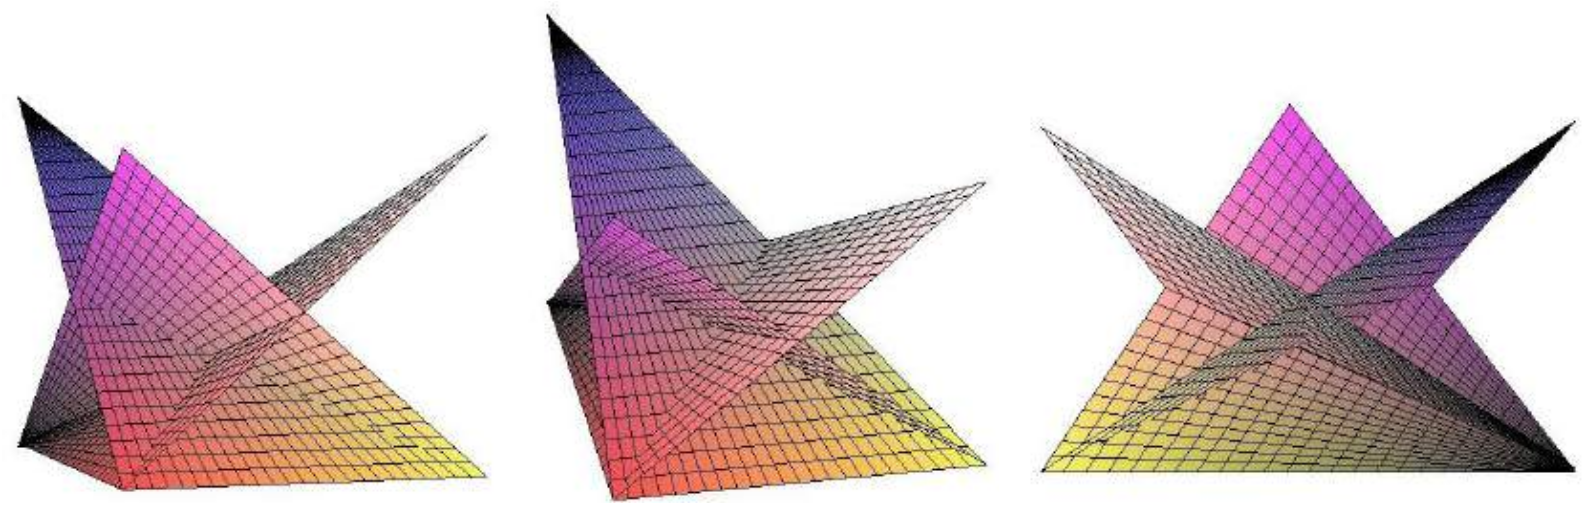
\includegraphics[scale=0.25]{./02_chaps/cap_mef/figure/tri_linear.png}
% \caption{Funções de Interpolação para o elemento triangular linear.}
% \label{tri_linear}
%\end{figure}


\medskip
\noindent
\textbf{Elemento triangular quadrático:} Geralmente este elemento é usado quando
possuímos restrições que impedem o uso do elemento linear ou quando estamos buscando uma
melhor aproximação do resultado. As matrizes elementares 
deste elemento são calculadas pela quadratura gaussiana cujos parâmetros podem ser
encontrados na literatura. Como se trata de um elemento quadrático, a ordem do polinômio 
interpolador é de grau dois. Desta forma, suas funções de interpolação são parabólicas.
Este elemento é representado pela \ref{elemento triangular quadrático}:

\begin{figure}[H]
\begin{center}
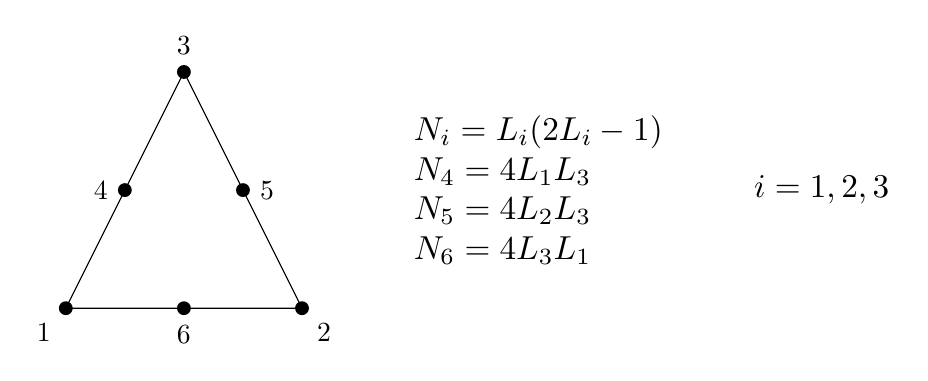
\begin{tikzpicture}[scale=3] 
 \draw (0,0) -- (1,0) -- (0.5,1) -- cycle;
 \node[circle, fill=black, inner sep=0pt, minimum size=5pt,label=below left:{1}] at (0,0) {};
 \node[circle, fill=black, inner sep=0pt, minimum size=5pt,label=below right:{2}] at (1,0) {};
 \node[circle, fill=black, inner sep=0pt, minimum size=5pt,label=above:{3}] at (0.5,1) {};
 \node[circle, fill=black, inner sep=0pt, minimum size=5pt,label=left:{4}] at (0.25,0.5) {};
 \node[circle, fill=black, inner sep=0pt, minimum size=5pt,label=right:{5}] at (0.75,0.5) {};
 \node[circle, fill=black, inner sep=0pt, minimum size=5pt,label=below:{6}] at (0.5,0.0) {};

 \node[draw=none, align=left, scale=1.2] at (2,0.5) {$N_i = L_i(2L_i - 1)$\\
                                                    $N_4 = 4L_1L_3$\\
                                                    $N_5 = 4L_2L_3$\\
                                                    $N_6 = 4L_3L_1$};

 \node[draw=none, scale=1.2] at (3.2,0.5) {$i = 1,2,3$};
\end{tikzpicture}
\end{center}
\caption{Elemento triangular quadrático}
\label{elemento triangular quadrático}
\end{figure}

\medskip
\noindent
\textbf{Elemento triangular cúbico:} Assim como o elemento quadrático, este elemento é usado quando
possuímos restrições que impedem o uso do elemento linear ou quando estamos buscando uma
melhor aproximação do resultado. Na literatura, este elemento é conhecido como \textit{elemento MINI}.
Suas matrizes elementares também são calculadas pela quadratura gaussiana. 
Como se trata de um elemento cúbico, a ordem do polinômio 
interpolador é de grau três. Desta forma, suas funções de interpolação possui
uma bolha no centro do elemento.
Este elemento é representado pela \ref{elemento triangular cúbico}:

\begin{figure}[H]
\begin{center}
\begin{tikzpicture}[scale=3] 
 \draw (0,0) -- (1,0) -- (0.5,1) -- cycle;
 \node[circle, fill=black, inner sep=0pt, minimum size=5pt,label=below left:{1}] at (0,0) {};
 \node[circle, fill=black, inner sep=0pt, minimum size=5pt,label=below right:{2}] at (1,0) {};
 \node[circle, fill=black, inner sep=0pt, minimum size=5pt,label=above:{3}] at (0.5,1) {};
 \node[circle, fill=black, inner sep=0pt, minimum size=5pt,label=above:{4}] at (1/2,1/3) {};
 
 \node[draw=none, align=left, scale=1.2] at (2,0.5) {$N_i = L_1 - 9L_1L_2L_3$\\
                                                    $N_4 = 27L_1L_2L_3$};

 \node[draw=none, scale=1.2] at (3.2,0.5) {$i = 1,2,3$};
\end{tikzpicture}
\end{center}
\caption{Elemento triangular cúbico}
\label{elemento triangular cúbico}
\end{figure}

%\begin{figure}[H]
%  \centering
%  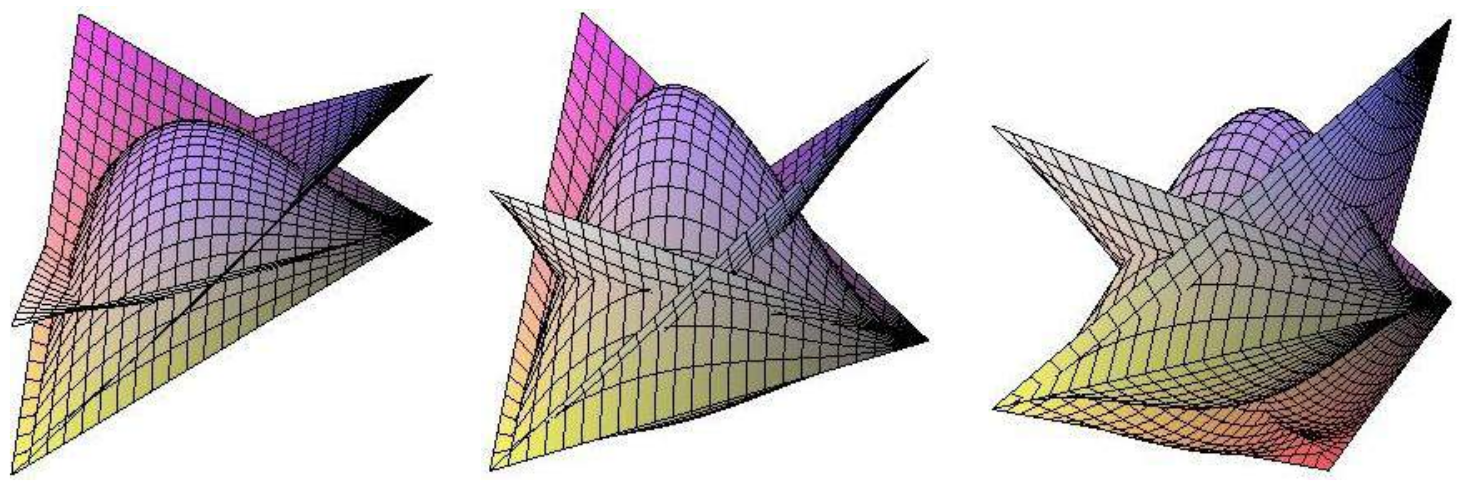
\includegraphics[scale=0.25]{./02_chaps/cap_mef/figure/mini.png}
% \caption{Funções de Interpolação para o elemento MINI.}
% \label{mini}
%\end{figure}

\medskip
\noindent
As Eqs (\ref{vorticity pre matrix} a \ref{concentration pre matrix}) podem ser representadas matricialmente por:

\begin{equation}
\begin{aligned}
 M \overset{.}{w} + u \cdot G_x w  + v \cdot G_y w & + \frac{1}{\textit{Re}} \Big[ K_{xx} + K_{yy} \Big] w
 \\[5pt]
 & + \frac{\Delta t}{2} u \Big[ u K_{xx} + v K_{yx} \Big] w 
 + \frac{\Delta t}{2} v \Big[ u K_{xy} + v K_{yy} \Big] w 
 = 0 \label{vorticity matrix}
\end{aligned}
\end{equation}

\begin{equation}
 - \Big[ K_{xx} + K_{yy} \Big] \psi + Mw = 0
\end{equation}

\begin{equation}
 Mu - G_y \psi = 0
\end{equation}

\begin{equation}
 Mv + G_x \psi = 0
\end{equation}

\begin{equation}
\begin{aligned}
 M \overset{.}{c} + u \cdot G_x c + v \cdot G_y c & + \frac{1}{\textit{ReSc}} \Big[ K_{xx} + K_{yy} \Big] c
 \\[5pt]
 & + \frac{\Delta t}{2} u \Big[ u K_{xx} + v K_{xy} \Big] c
 + \frac{\Delta t}{2} v \Big[ u K_{yx} + v K_{yy} \Big] c 
 = 0 \label{concentration matrix}
\end{aligned} 
\end{equation}

\medskip
\noindent
onde as matrizes \textbf{M}, \textbf{G\textsubscript{x}}, 
\textbf{G\textsubscript{y}}, \textbf{K\textsubscript{xx}},
\textbf{K\textsubscript{xy}},
\textbf{K\textsubscript{yx}}, 
\textbf{K\textsubscript{yy}}, 
possuem dimensões \textbf{np} x \textbf{np}
(isto é, número de nós por número de nós) e
são definidas como:

\begin{align}
  \textbf{M} & = \textbf{A} m^{e}\\
  \textbf{G\textsubscript{x}} & = \textbf{A} g_{x}^{e}\\
  \textbf{G\textsubscript{y}} & = \textbf{A} g_{y}^{e} \\
  \textbf{K\textsubscript{xx}} & = \textbf{A} k_{xx}^{e} \\
  \textbf{K\textsubscript{xy}} & = \textbf{A} k_{xy}^{e} \\
  \textbf{K\textsubscript{yx}} & = \textbf{A} k_{yx}^{e} \\
  \textbf{K\textsubscript{yy}} & = \textbf{A} k_{yy}^{e}
\end{align}

\noindent
onde \textbf{A} é um operador de montagem das
matrizes elementares nas matrizes globais, 
respeitando a correspondência entre os índices
globais e locais e 
$m^{e}$, 
$g^{e}_{x}$,
$g^{e}_{y}$,
$k^{e}_{xx}$,
$k^{e}_{xy}$,
$k^{e}_{yx}$,
$k^{e}_{yy}$
são as matrizes elementares cuja dimensão para o 
\textit{elemento triangular linear} é \textit{3}x\textit{3} e 
são definidas por:


\begin{equation}
 \begin{aligned}
  m^{e} & = \int_{\Omega^{e}} N_{i}^{e} N_{j}^{e} d\Omega \\
  g_{x}^{e} & = \int_{\Omega^{e}} \frac{\partial N_{i}^{e}}{\partial x} N_{j}^{e} d\Omega \\
  g_{y}^{e} & = \int_{\Omega^{e}} \frac{\partial N_{i}^{e}}{\partial y} N_{j}^{e} d\Omega \\
  k_{xx}^{e} & = \int_{\Omega^{e}} \frac{\partial N_{i}^{e}}{\partial x} \frac{\partial N_{j}^{e}}{\partial x} \\
  k_{xy}^{e} & = \int_{\Omega^{e}} \frac{\partial N_{i}^{e}}{\partial x} \frac{\partial N_{j}^{e}}{\partial y} \\
  k_{yx}^{e} & = \int_{\Omega^{e}} \frac{\partial N_{i}^{e}}{\partial y} \frac{\partial N_{j}^{e}}{\partial x} \\
  k_{yy}^{e} & = \int_{\Omega^{e}} \frac{\partial N_{i}^{e}}{\partial y} \frac{\partial N_{j}^{e}}{\partial y}
 \end{aligned}
\end{equation}

\medskip
Sendo assim, as equações de governo em sua forma matricial discretizadas
segundo o Método dos Elementos Finitos que usamos neste trabalho foram:

\begin{equation} \label{final equation}
\begin{aligned}
 \frac{M}{\Delta t} w^{n+1} = \frac{M}{\Delta t} w^{n} - u \cdot G_x w^{n} & - v \cdot G_y w^{n} 
 - \frac{1}{\textit{Re}} \Big[ K_{xx} + K_{yy} \Big] w^{n}  
 \\[5pt]
 & - \frac{\Delta t}{2} u \Big[ u K_{xx} + v K_{yx} \Big] w^{n} 
 - \frac{\Delta t}{2} v \Big[ u K_{xy} + v K_{yy} \Big] w^{n} 
\end{aligned}
\end{equation}


\begin{equation}
 \Big[ K_{xx} + K_{yy} \Big] \psi = Mw
\end{equation}

\begin{equation}
 Mu = G_y \psi
\end{equation}

\begin{equation}
 Mv = - G_x \psi
\end{equation}

\begin{equation}
\begin{aligned}
 \frac{M}{\Delta t} c^{n+1} = \frac{M}{\Delta t} c^{n}  - u \cdot G_x c^{n} - v & \cdot G_y c^{n} 
 - \frac{1}{\textit{ReSc}} \Big[ K_{xx} + K_{yy} \Big] c^{n}  
 \\[5pt]
 & - \frac{\Delta t}{2} u \Big[ u K_{xx} + v K_{yx} \Big] c^{n} 
 - \frac{\Delta t}{2} v \Big[ u K_{xy} + v K_{yy} \Big] c^{n} 
\end{aligned}
\end{equation}



\chapter{\textbf{COMPUTATIONAL CODE}}
\label{codigo numerico}

\section{\textbf{Introduction}} 
In this chapter, we will present the main characteristics 
of the computational code developed in Python 2.7 \cite{python} 
using the object-oriented paradigm (OOP) in order to reuse the code 
in other simulations in the future. All developed classes are imported 
into the simulator (\textit{TriSim}), where the result of the 
numerical simulation is exported as presented in the 
simplified \textit{Class Diagram} (UML) of \ref{uml}. 
Initially, the \textit{script} that performs the import 
of the computational mesh for the simulation is presented. 
Then, the assembly of the global matrices is done 
respecting the correspondence between the global and local index. 
Later on, we present the application of boundary conditions for 
both \textit{Dirichlet} and \textit{Neumann}. 
Finally, the solve algorithm for the vorticity-streamfunction 
formulation with the species transport equation is presented.

\vspace{0.5cm}
\begin{figure}[H]
\begin{center}
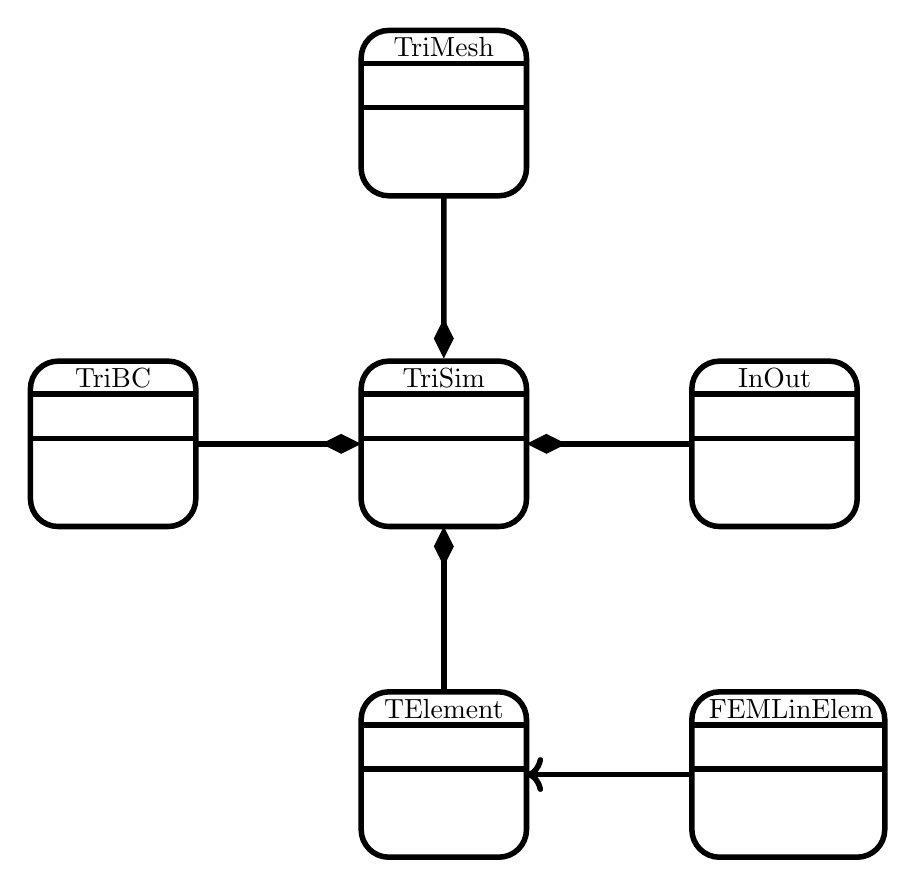
\begin{tikzpicture}[scale=0.7pt]
 \draw [rounded corners=10,line width=2pt] (0,0) rectangle ++(3,3);
 \draw [line width=2pt] (0,2.4) -- (3,2.4);
 \draw [line width=2pt] (0,1.6) -- (3,1.6);
 \node (TriSim) at (1.5,2.7) {TriSim};

 \draw [rounded corners=10,line width=2pt] (0,6) rectangle ++(3,3);
 \draw [line width=2pt] (0,8.4) -- (3,8.4);
 \draw [line width=2pt] (0,7.6) -- (3,7.6);
 \node (TriMesh) at (1.5,8.7) {TriMesh};

 \draw [rounded corners=10,line width=2pt] (6,0) rectangle ++(3,3);
 \draw [line width=2pt] (6,2.4) -- (9,2.4);
 \draw [line width=2pt] (6,1.6) -- (9,1.6);
 \node (InOut) at (7.5,2.7) {InOut};

 \draw [rounded corners=10,line width=2pt] (-6,0) rectangle ++(3,3);
 \draw [line width=2pt] (-6,2.4) -- (-3,2.4);
 \draw [line width=2pt] (-6,1.6) -- (-3,1.6);
 \node (triBC) at (-4.5,2.7) {TriBC};

 \draw [rounded corners=10,line width=2pt] (0,-6) rectangle ++(3,3);
 \draw [line width=2pt] (0,-3.6) -- (3,-3.6);
 \draw [line width=2pt] (0,-4.4) -- (3,-4.4);
 \node (TElement) at (1.5,-3.3) {TElement};

 \draw [rounded corners=10,line width=2pt] (6,-6) rectangle ++(3.5,3);
 \draw [line width=2pt] (6,-3.6) -- (9.5,-3.6);
 \draw [line width=2pt] (6,-4.4) -- (9.5,-4.4);
 \node (FEMLinElement) at (7.8,-3.3) {FEMLinElem};

 \draw [{Diamond}-,line width=2pt] (TriSim) -- (1.5,6);
 \draw [{Diamond}-,line width=2pt] (0,1.5) -- (-3,1.5);
 \draw [{Diamond}-,line width=2pt] (1.5,0) -- (1.5,-3);
 \draw [{Diamond}-,line width=2pt] (3,1.5) -- (6,1.5);
 \draw [<-,line width=2pt] (3,-4.5) -- (6,-4.5);

\end{tikzpicture}
\end{center}
\caption{Simplified Class Diagram}
\label{uml}
\end{figure}


\section{\textbf{Mesh Import}} 
\label{trimesh}

The domain consists of an unstructured mesh generated by 
the \textit{GMSH} open-source software proposed by 
Geuzaine and Remacle (2009) \cite{gmsh} and 
it was imported into the numerical simulation by 
the \textit{TriMesh} class. 
Initially, we used a well-known computational community script to 
convert the \textit{.msh} file to a 
\textit{Python} list:

\begin{verbatim}
__________________________________________________________________________
mesh = []                             | python list inicialization
with open("file.msh") as mesh:        | open file 
 for line in mesh:                    | loop file each line
  row = line.split()                  | split file line
  mesh.append(row[:])                 | add file line from python list 
__________________________________________________________________________
\end{verbatim}

\noindent
Then, this class returns important information for the simulation 
such as:
\textit{nodes number} (\textbf{np}), 
\textit{elements number} (\textbf{ne}), 
\textit{the coordinate vectors} (\textbf{x} and \textbf{y}), 
\textit{the connectivity matrix} (\textbf{IEN}) and 
\textit{the Boundary nodes}. 
The \ref{tempo malha} shows the average processing time for 
mesh import in several unstructured linear triangular meshes import.

\vspace{0.5cm}
\begin{table}[H]
\centering
\begin{tabular}{ccc}
\toprule
\textbf{Nodes} & \textbf{Elements} & \textbf{AVG Processing Time} (s) \\
\midrule
10482 & 20142 & 0,6 \\
40819 & 80005 & 2,6 \\
249677 & 495289 & 16,6 \\
993091 & 2010501 & 70,4 \\
\bottomrule
\end{tabular}
\caption{Average processing time for mesh import in several unstructured linear triangular meshes}
\label{tempo malha}
\end{table}

\newpage


\section{\textbf{Matrix Assemble}} 
\label{trielem}

After importing the \textit{.msh} file, the global arrays 
were assembled. They were initialized as sparse matrices by 
the \textit{Scipy} library \cite{scipy} and the following 
\textit{script} was used for the assembly:

%\begin{algorithm}[H]
%\caption{Assembly Global Matrix}
%\begin{algorithmic}
% \For {e in range(0,ne)}
%   \State Linear\_Element\\
%   \For {i in range(0,3)}
%    \State ii = IEN[e][i]\\
%    \For {j in range(0,3)}
%     \State jj = IEN[e][j]\\
%     \State Kxx[ii][jj] += kxx\_element[i][j]
%     \State Kxy[ii][jj] += kxy\_element[i][j]
%    \State Kyx[ii][jj] += kyx\_element[i][j]
%    \State Kyy[ii][jj] += kyy\_element[i][j]
%    \State Gx[ii][jj] += gx\_element[i][j]
%    \State Gy[ii][jj] += gy\_element[i][j]
%    \State M[ii][jj] += mass\_element[i][j]\\
%   \EndFor 
%  \EndFor 
% \EndFor 
%\end{algorithmic}
%\end{algorithm}


\begin{verbatim}
__________________________________________________________________________
for e in range(0, ne):                      | element loop 
 linear_element(e)                          | elementary matrix
                                              by gaussian quadrature

 for i in range(0,3):                       
  ii = IEN[e][i]                            
  
  for j in range(0,3):                       
   jj = IEN[e][j]
                                            
   Kxx[ii,jj] += kxx_element[i][j]          |
   Kxy[ii,jj] += kxy_element[i][j]          |
   Kyx[ii,jj] += kyx_element[i][j]          |
   Kyy[ii,jj] += kyy_element[i][j]          | globals matrices assembly
                                            | with global and local 
   Gx[ii,jj] += gx_element[i][j]            | index correspondence
   Gy[ii,jj] += gy_element[i][j]            | 
                                            |
   M[ii,jj] += mass_element[i][j]           |
__________________________________________________________________________
\end{verbatim}


\medskip
The assembly of the elementary matrices is done by the module 
\textit{linear\_element} whose required parameter is the 
element number. This module is part of the \textit{TElement} 
class where it uses the Gaussian Quadrature to calculate 
the values of the elementary matrices. For the linear 
triangular element, it is also possible to use elementary 
analytical matrices. For more details consult the work of Lewis, 
Nithiarasu and Seetharamu (2004) \cite{lewis2004}.

\newpage
Then, the left hand matrix known as \textit {left hand side (LHS)} 
is created for the streamfunction, velocity and concentration equations 
respectively:

\begin{verbatim}
__________________________________________________________________________
LHS_psi = sps.lil_matrix.copy(K)
LHS_vx = sps.lil_matrix.copy(M)
LHS_vy = sps.lil_matrix.copy(M)
LHS_c = sps.lil_matrix.copy(M)/dt
__________________________________________________________________________
\end{verbatim}

The \textit{LHS} matrix for the vorticity equation is created 
during the solution algorithm loop to ensure that it will always 
be initialized using the original global matrices. 
It is necessary to use the function \textit{copy} because 
we want to copy the values of the global arrays and not reference them, 
for more details consult the \textit{Scipy Community} \cite{numpycopy}. 
The \ref{tempo matrizes globais} shows the average processing time 
for global matrices assembly in several unstructured linear 
triangular meshes.


\vspace{0.5cm}
\begin{table}[H]
\centering
\begin{tabular}{ccc}
\toprule
\textbf{Nodes} & \textbf{Elements} & \textbf{AVG Processing Time} (s) \\
\midrule
10482 & 20142 & 72,9 \\
40819 & 80005 & 254,3 \\
249677 & 495289 & 1664,9 \\
993091 & 2010501 & 69059,9 \\

\bottomrule
\end{tabular}
\caption{Average processing time for global matrices assembly in several unstrutured linear triangular meshes}
\label{tempo matrizes globais}
\end{table}
                


\section{\textbf{Boundary Condition Apply}} 
\label{tricond}

After the global matrices assembly, the boundary conditions are applied. 
As was said in the section \ref{trimesh}, during the mesh import 
it is possible to identify the nodes that they are in the boundary. 
The condition where the nodes have their values predefined 
by the problem is known as \textit{Dirichlet condition}. 
Therefore, these nodes must not be changed as the simulation is 
performed. In this way, the product between the column of the 
global matrix whose index is a node with Dirichlet boundary condition 
and its predefined value as boundary condition is subtracted from 
the vector on the right side of the governing equation. 
Then, we zero the rows and columns of the global matrix that 
corresponds to the condition index of Dirichlet and we set the value 
of 1 on the main diagonal.

\medskip
Para exemplificar, consideraremos uma matriz 
com dimensões (\textit{np x np})
e o nó 2 como um nó localizado no
contorno do domínio onde a condição proposta
é de Dirichlet.
Desta forma, o seguinte algoritmo é feito conforme apresentado por Anjos (2007) \cite{anjos2007}:

\begin{enumerate}
 
 \vspace{0.5cm}
 \item \textbf{Localiza-se o nó de condição de contorno na matriz:}
\medskip
\begin{center}
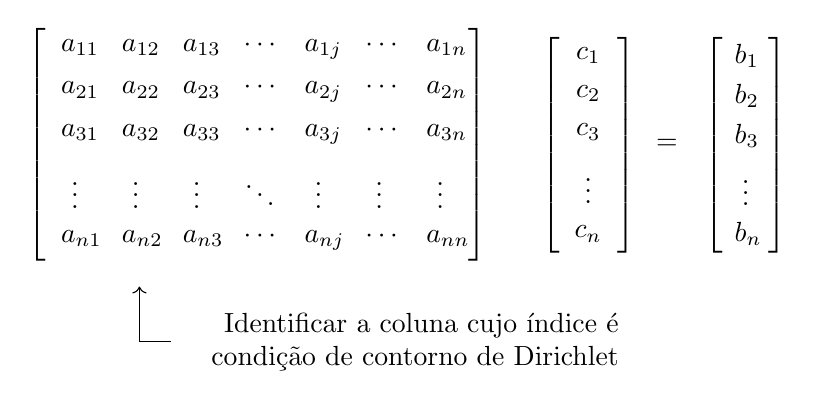
\begin{tikzpicture}
\matrix (m) [matrix of math nodes,
inner sep=0pt, column sep=0.4em,
nodes={inner sep=0.4em,text width=1.0em,align=center},
left delimiter={[},
right delimiter={]},
]
{
a_{11} & a_{12} & a_{13} & \cdots & a_{1j} & \cdots & a_{1n} \\
a_{21} & a_{22} & a_{23} & \cdots & a_{2j} & \cdots & a_{2n} \\
a_{31} & a_{32} & a_{33} & \cdots & a_{3j} & \cdots & a_{3n} \\
\vdots & \vdots & \vdots & \ddots & \vdots & \vdots & \vdots \\
a_{n1} & a_{n2} & a_{n3} & \cdots & a_{nj} & \cdots & a_{nn} \\
};
\begin{scope}[xshift=4.2cm]
\matrix (m) [matrix of math nodes,
inner sep=0pt, column sep=0.4em,
nodes={inner sep=0.4em,text width=1em,align=center},
left delimiter={[},
right delimiter={]},
]
{
c_1 \\
c_2 \\
c_3 \\
\vdots \\
c_n \\
};
\end{scope}
\begin{scope}[xshift=5.2cm]
\node {=};
\end{scope}
\begin{scope}[xshift=6.2cm]
\matrix (m) [matrix of math nodes,
inner sep=0pt, column sep=0.4em,
nodes={inner sep=0.3em,text width=0.8em,align=center},
left delimiter={[},
right delimiter={]},
]
{
b_1 \\
b_2 \\
b_3 \\
\vdots \\
b_n \\
};
\end{scope}
 \draw[<-] (-1.5,-1.8) -- (-1.5,-2.5) -- (-1.1,-2.5);
 \node [draw=none, align=right] at (2.0,-2.5) {Identificar a coluna cujo índice é \\ condição de contorno de Dirichlet};
\end{tikzpicture}
\end{center}

 \vspace{0.5cm}
 \item \textbf{Subtrai-se o produto entre a coluna onde está situado o nó da matriz e o seu valor pré definido 
com o vetor do lado direito da equação:}
\medskip
\begin{center}
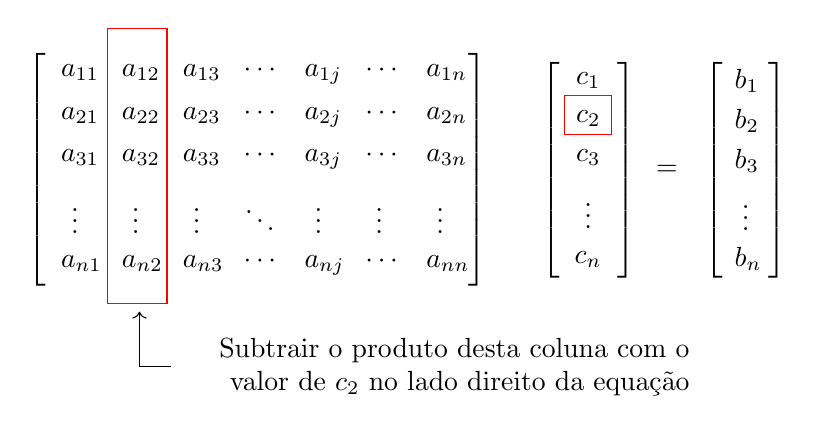
\begin{tikzpicture}
\matrix (m) [matrix of math nodes,
inner sep=0pt, column sep=0.4em,
nodes={inner sep=0.4em,text width=1.0em,align=center},
left delimiter={[},
right delimiter={]},
]
{
a_{11} & a_{12} & a_{13} & \cdots & a_{1j} & \cdots & a_{1n} \\
a_{21} & a_{22} & a_{23} & \cdots & a_{2j} & \cdots & a_{2n} \\
a_{31} & a_{32} & a_{33} & \cdots & a_{3j} & \cdots & a_{3n} \\
\vdots & \vdots & \vdots & \ddots & \vdots & \vdots & \vdots \\
a_{n1} & a_{n2} & a_{n3} & \cdots & a_{nj} & \cdots & a_{nn} \\
};
\begin{scope}[xshift=4.2cm]
\matrix (m) [matrix of math nodes,
inner sep=0pt, column sep=0.4em,
nodes={inner sep=0.4em,text width=1em,align=center},
left delimiter={[},
right delimiter={]},
]
{
c_1 \\
c_2 \\
c_3 \\
\vdots \\
c_n \\
};
\end{scope}
\begin{scope}[xshift=5.2cm]
\node {=};
\end{scope}
\begin{scope}[xshift=6.2cm]
\matrix (m) [matrix of math nodes,
inner sep=0pt, column sep=0.4em,
nodes={inner sep=0.3em,text width=0.8em,align=center},
left delimiter={[},
right delimiter={]},
]
{
b_1 \\
b_2 \\
b_3 \\
\vdots \\
b_n \\
};
\end{scope}
 %text
 \draw[<-] (-1.5,-1.8) -- (-1.5,-2.5) -- (-1.1,-2.5);
 \node [draw=none, align=right] at (2.5,-2.5) {Subtrair o produto desta coluna com o \\ valor de $c_2$ no lado direito da equação};
 %block
 \draw[red] (-1.9,1.8) -- (-1.15,1.8) -- (-1.15,-1.7) -- (-1.9,-1.7) -- cycle;
 \draw[red] (3.9,0.95) -- (4.5,0.95) -- (4.5,0.45) -- (3.9,0.45) -- cycle;
\end{tikzpicture}
\end{center}

\newpage
isto é,

\medskip
\begin{center}
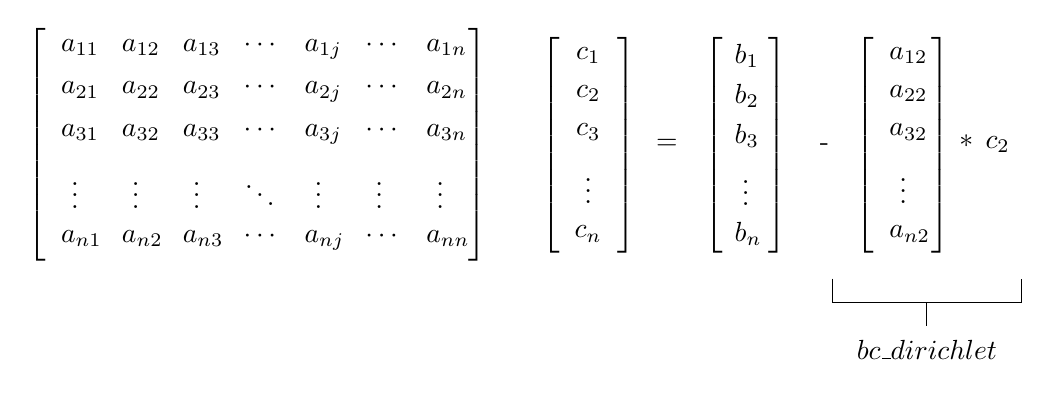
\begin{tikzpicture}
\matrix (m) [matrix of math nodes,
inner sep=0pt, column sep=0.4em,
nodes={inner sep=0.4em,text width=1.0em,align=center},
left delimiter={[},
right delimiter={]},
]
{
a_{11} & a_{12} & a_{13} & \cdots & a_{1j} & \cdots & a_{1n} \\
a_{21} & a_{22} & a_{23} & \cdots & a_{2j} & \cdots & a_{2n} \\
a_{31} & a_{32} & a_{33} & \cdots & a_{3j} & \cdots & a_{3n} \\
\vdots & \vdots & \vdots & \ddots & \vdots & \vdots & \vdots \\
a_{n1} & a_{n2} & a_{n3} & \cdots & a_{nj} & \cdots & a_{nn} \\
};
\begin{scope}[xshift=4.2cm]
\matrix (m) [matrix of math nodes,
inner sep=0pt, column sep=0.4em,
nodes={inner sep=0.4em,text width=1em,align=center},
left delimiter={[},
right delimiter={]},
]
{
c_1 \\
c_2 \\
c_3 \\
\vdots \\
c_n \\
};
\end{scope}
\begin{scope}[xshift=5.2cm]
\node {=};
\end{scope}
\begin{scope}[xshift=6.2cm]
\matrix (m) [matrix of math nodes,
inner sep=0pt, column sep=0.4em,
nodes={inner sep=0.3em,text width=0.8em,align=center},
left delimiter={[},
right delimiter={]},
]
{
b_1 \\
b_2 \\
b_3 \\
\vdots \\
b_n \\
};
\end{scope}
\begin{scope}[xshift=7.2cm]
\node {-};
\end{scope}
\begin{scope}[xshift=8.2cm]
\matrix (m) [matrix of math nodes,
inner sep=0pt, column sep=0.4em,
nodes={inner sep=0.4em,text width=1em,align=center},
left delimiter={[},
right delimiter={]},
]
{
a_{12} \\
a_{22} \\
a_{32} \\
\vdots \\
a_{n2} \\
};
\end{scope}
\begin{scope}[xshift=9.0cm]
\node {*};
\end{scope}
\begin{scope}[xshift=9.4cm]
 \node {$c_2$};
\end{scope}
 %text
 \node [draw=none, align=right] at (8.5,-2.6) {$bc\_dirichlet$};
 %block
 \draw (7.3,-1.7) -- (7.3,-2.0) -- (9.7,-2.0) -- (9.7,-1.7);
 \draw (8.5,-2.0) -- (8.5,-2.3);
\end{tikzpicture}
\end{center}

 \vspace{0.5cm}
 \item \textbf{Preenche-se com zeros a coluna e a linha da matriz correspondente ao nó de condição de contorno:}
\medskip
\begin{center}
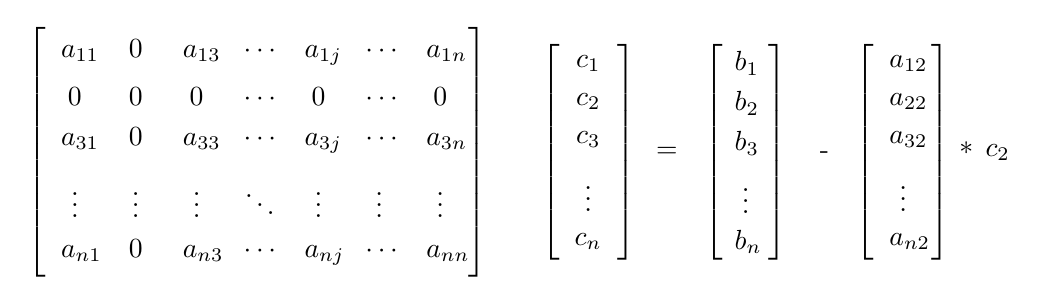
\begin{tikzpicture}
\matrix (m) [matrix of math nodes,
inner sep=0pt, column sep=0.4em,
nodes={inner sep=0.4em,text width=1.0em,align=center},
left delimiter={[},
right delimiter={]},
]
{
a_{11} & 0 & a_{13} & \cdots & a_{1j} & \cdots & a_{1n} \\
0 & 0 & 0 & \cdots & 0 & \cdots & 0 \\
a_{31} & 0 & a_{33} & \cdots & a_{3j} & \cdots & a_{3n} \\
\vdots & \vdots & \vdots & \ddots & \vdots & \vdots & \vdots \\
a_{n1} & 0 & a_{n3} & \cdots & a_{nj} & \cdots & a_{nn} \\
};
\begin{scope}[xshift=4.2cm]
\matrix (m) [matrix of math nodes,
inner sep=0pt, column sep=0.4em,
nodes={inner sep=0.4em,text width=1em,align=center},
left delimiter={[},
right delimiter={]},
]
{
c_1 \\
c_2 \\
c_3 \\
\vdots \\
c_n \\
};
\end{scope}
\begin{scope}[xshift=5.2cm]
\node {=};
\end{scope}
\begin{scope}[xshift=6.2cm]
\matrix (m) [matrix of math nodes,
inner sep=0pt, column sep=0.4em,
nodes={inner sep=0.3em,text width=0.8em,align=center},
left delimiter={[},
right delimiter={]},
]
{
b_1 \\
b_2 \\
b_3 \\
\vdots \\
b_n \\
};
\end{scope}
\begin{scope}[xshift=7.2cm]
\node {-};
\end{scope}
\begin{scope}[xshift=8.2cm]
\matrix (m) [matrix of math nodes,
inner sep=0pt, column sep=0.4em,
nodes={inner sep=0.4em,text width=1em,align=center},
left delimiter={[},
right delimiter={]},
]
{
a_{12} \\
a_{22} \\
a_{32} \\
\vdots \\
a_{n2} \\
};
\end{scope}
\begin{scope}[xshift=9.0cm]
\node {*};
\end{scope}
\begin{scope}[xshift=9.4cm]
 \node {$c_2$};
\end{scope}
\end{tikzpicture}
\end{center}


 \vspace{0.5cm}
 \item \textbf{Coloca-se 1 na diagonal principal da matriz cujo índice é o nó de condição de contorno:}
\medskip
\begin{center}
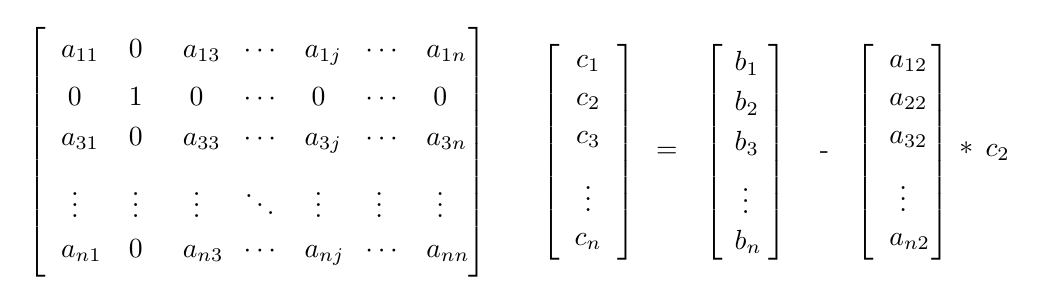
\begin{tikzpicture}
\matrix (m) [matrix of math nodes,
inner sep=0pt, column sep=0.4em,
nodes={inner sep=0.4em,text width=1.0em,align=center},
left delimiter={[},
right delimiter={]},
]
{
a_{11} & 0 & a_{13} & \cdots & a_{1j} & \cdots & a_{1n} \\
0 & 1 & 0 & \cdots & 0 & \cdots & 0 \\
a_{31} & 0 & a_{33} & \cdots & a_{3j} & \cdots & a_{3n} \\
\vdots & \vdots & \vdots & \ddots & \vdots & \vdots & \vdots \\
a_{n1} & 0 & a_{n3} & \cdots & a_{nj} & \cdots & a_{nn} \\
};
\begin{scope}[xshift=4.2cm]
\matrix (m) [matrix of math nodes,
inner sep=0pt, column sep=0.4em,
nodes={inner sep=0.4em,text width=1em,align=center},
left delimiter={[},
right delimiter={]},
]
{
c_1 \\
c_2 \\
c_3 \\
\vdots \\
c_n \\
};
\end{scope}
\begin{scope}[xshift=5.2cm]
\node {=};
\end{scope}
\begin{scope}[xshift=6.2cm]
\matrix (m) [matrix of math nodes,
inner sep=0pt, column sep=0.4em,
nodes={inner sep=0.3em,text width=0.8em,align=center},
left delimiter={[},
right delimiter={]},
]
{
b_1 \\
b_2 \\
b_3 \\
\vdots \\
b_n \\
};
\end{scope}
\begin{scope}[xshift=7.2cm]
\node {-};
\end{scope}
\begin{scope}[xshift=8.2cm]
\matrix (m) [matrix of math nodes,
inner sep=0pt, column sep=0.4em,
nodes={inner sep=0.4em,text width=1em,align=center},
left delimiter={[},
right delimiter={]},
]
{
a_{12} \\
a_{22} \\
a_{32} \\
\vdots \\
a_{n2} \\
};
\end{scope}
\begin{scope}[xshift=9.0cm]
\node {*};
\end{scope}
\begin{scope}[xshift=9.4cm]
 \node {$c_2$};
\end{scope}
\end{tikzpicture}
\end{center}

 \vspace{0.5cm}
 \item \textbf{Localiza-se o próximo nó e executa-se o passo novamente.}
\end{enumerate}

\newpage
\noindent
A implementação deste algoritmo foi realizado pelo seguinte \textit{script}:
\begin{verbatim}
__________________________________________________________________________
 for mm in ibc:                        | loop sobre os nós do contorno
  bc_dirichlet -= LHS[:,mm]*bc_1[mm]   | passo 2
  LHS[:,mm] = 0.0                      | passo 3 - zerar colunas
  LHS[mm,:] = 0.0                      | passo 3 - zerar linhas
  LHS[mm,mm] = 1.0                     | passo 4 - 1 na diagonal principal
  bc_dirichlet[mm] = bc_1[mm]          | imputando o valor da condição
                                       | de Dirichlet no índice
                                       | correspondente
__________________________________________________________________________
\end{verbatim}

\noindent
onde \textit{ibc} é uma lista que contém todos os nós do contorno
cuja condição é de Dirichlet e
\textit{$bc\_1$} é um vetor auxiliar com dimensão \textit{np}
onde o valor da condição de Dirichlet é imputada em cada índice correspondente.
O símbolo -= garante que a contribuição de cada nó cuja
condição seja de Dirichlet seja computada.
Este procedimento deverá ser realizado para cada um das \textit{LHS}.
A \ref{tempo contorno} apresenta o tempo de processamento para 
a aplicação das condições de contorno de \textit{Dirichlet} em diversas
malhas triangulares lineares não estruturadas.

\vspace{0.5cm}
\begin{table}[H]
\centering
\begin{tabular}{ccc}
\toprule
\textbf{N. Nós} & \textbf{N. Elementos} & \textbf{Tempo de Processamento} (s) \\
\midrule
10482 & 20142 & 6,8 \\
40819 & 80005 & 37,5 \\
249677 & 495289 & 467,7 \\
993091 & 2010501 & 3720,6 \\
\bottomrule
\end{tabular}
\caption{Tempo processamento para as condições de contorno para diversas malhas triangulares não estruturadas}
\label{tempo contorno}
\end{table}
 

\medskip
Outro tipo de condição de contorno muito comum é aquela onde existe um
fluxo nos contornos do domínio. Essa condição de contorno é conhecida
como \textit{Condição de Neumann} e na formulação variacional é chamada
de \textit{Condição Natural}. Diferente da condição de Dirichlet,
esse tipo de condição de contorno não afeta a matriz global do lado esquerdo quando
o fluxo é constante. Devemos apenas somar a sua contribuição
no vetor do lado direito da equação, isto é:

\begin{center}
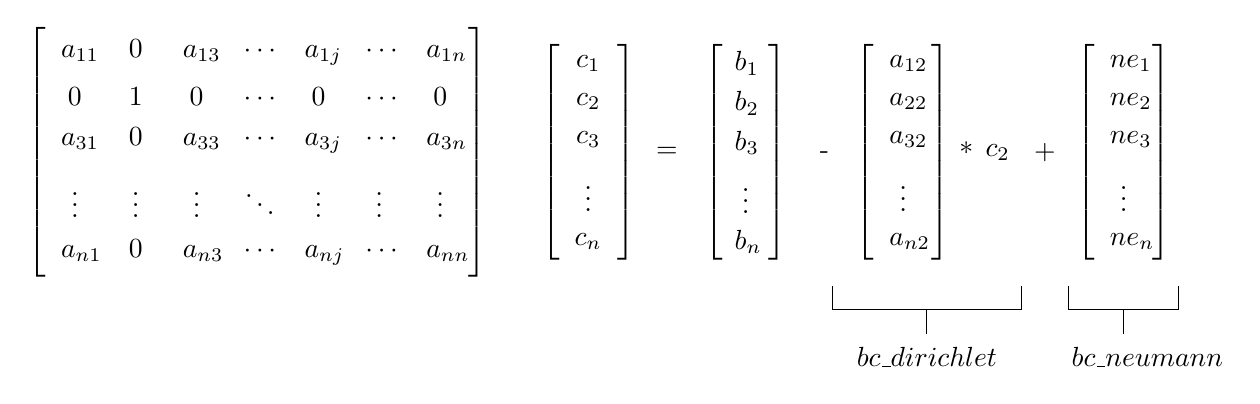
\begin{tikzpicture}
\matrix (m) [matrix of math nodes,
inner sep=0pt, column sep=0.4em,
nodes={inner sep=0.4em,text width=1.0em,align=center},
left delimiter={[},
right delimiter={]},
]
{
a_{11} & 0 & a_{13} & \cdots & a_{1j} & \cdots & a_{1n} \\
0 & 1 & 0 & \cdots & 0 & \cdots & 0 \\
a_{31} & 0 & a_{33} & \cdots & a_{3j} & \cdots & a_{3n} \\
\vdots & \vdots & \vdots & \ddots & \vdots & \vdots & \vdots \\
a_{n1} & 0 & a_{n3} & \cdots & a_{nj} & \cdots & a_{nn} \\
};
\begin{scope}[xshift=4.2cm]
\matrix (m) [matrix of math nodes,
inner sep=0pt, column sep=0.4em,
nodes={inner sep=0.4em,text width=1em,align=center},
left delimiter={[},
right delimiter={]},
]
{
c_1 \\
c_2 \\
c_3 \\
\vdots \\
c_n \\
};
\end{scope}
\begin{scope}[xshift=5.2cm]
\node {=};
\end{scope}
\begin{scope}[xshift=6.2cm]
\matrix (m) [matrix of math nodes,
inner sep=0pt, column sep=0.4em,
nodes={inner sep=0.3em,text width=0.8em,align=center},
left delimiter={[},
right delimiter={]},
]
{
b_1 \\
b_2 \\
b_3 \\
\vdots \\
b_n \\
};
\end{scope}
\begin{scope}[xshift=7.2cm]
\node {-};
\end{scope}
\begin{scope}[xshift=8.2cm]
\matrix (m) [matrix of math nodes,
inner sep=0pt, column sep=0.4em,
nodes={inner sep=0.4em,text width=1em,align=center},
left delimiter={[},
right delimiter={]},
]
{
a_{12} \\
a_{22} \\
a_{32} \\
\vdots \\
a_{n2} \\
};
\end{scope}
\begin{scope}[xshift=9.0cm]
\node {*};
\end{scope}
\begin{scope}[xshift=9.4cm]
 \node {$c_2$};
\end{scope}
\begin{scope}[xshift=10.0cm]
\node {+};
\end{scope}
\begin{scope}[xshift=11.0cm]
\matrix (m) [matrix of math nodes,
inner sep=0pt, column sep=0.4em,
nodes={inner sep=0.4em,text width=1em,align=center},
left delimiter={[},
right delimiter={]},
]
{
ne_{1} \\
ne_{2} \\
ne_{3} \\
\vdots \\
ne_{n} \\
};
\end{scope}
 %text
 \node [draw=none, align=right] at (8.5,-2.6) {$bc\_dirichlet$};
 \node [draw=none, align=right] at (11.3,-2.6) {$bc\_neumann$};
 %block
 \draw (7.3,-1.7) -- (7.3,-2.0) -- (9.7,-2.0) -- (9.7,-1.7);
 \draw (8.5,-2.0) -- (8.5,-2.3);
 \draw (10.3,-1.7) -- (10.3,-2.0) -- (11.7,-2.0) -- (11.7,-1.7);
 \draw (11.0,-2.0) -- (11.0,-2.3);
\end{tikzpicture}
\end{center}

\medskip
Como foi mencionado no capítulo \ref{metodo dos elementos finitos}, possuímos apenas condição de Dirichlet neste trabalho.
A seguir, porém, apresentaremos a implementação desse tipo de condição.
A fim de exemplificar, consideraremos o termo de contorno da equação
\ref{diffusion2_concentration}, isto é:

\begin{equation} 
 \frac{1}{\textit{ReSc}} \int_{\Gamma} \eta \nabla c \cdot \textbf{n} d\Gamma
\end{equation}

\medskip
\noindent
onde $\nabla c$ é o fluxo que será considerado constante. 
Após a discretização pela formulação de Galerkin, 
possuímos a seguinte expressão:

\begin{equation} 
 \frac{1}{\textit{ReSc}} \int_{\Gamma} N_j \nabla c \cdot \textbf{n} d\Gamma
\end{equation}

\medskip
\noindent
isto é:

\begin{equation} 
 \frac{1}{\textit{ReSc}} \Bigg[ \frac{length  \nabla c}{2} \Bigg]
\end{equation}

\medskip
\noindent
onde a variável \textit{$length$} é o comprimento da aresta do elemento. 
Considerando um domínio bidimensional onde 
\textit{$i$} é um nó no contorno deste domínio e
\textit{$i-1$} e \textit{$i+1$} são seus vizinhos neste contorno,
as arestas do nó \textit{$i$} podem ser
representadas por:

\begin{figure}[h!]
\begin{center}
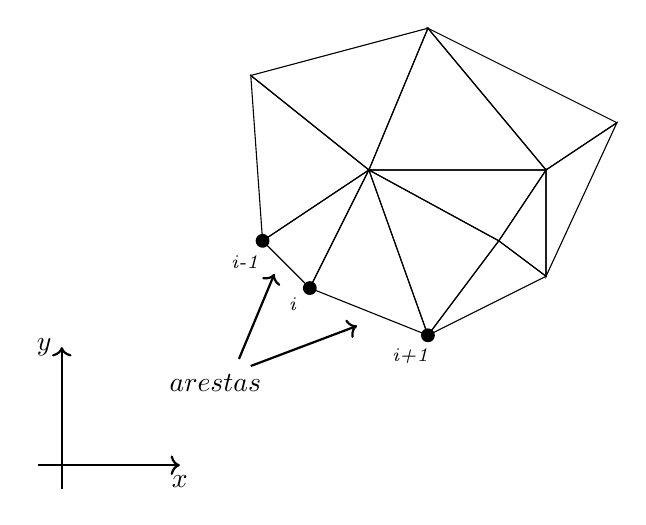
\begin{tikzpicture}[scale=3]
 \draw (0.75,0.75) -- (1.25,0.55) -- (1.00,1.25) -- cycle;
 \draw (0.75,0.75) -- (0.55,0.95) -- (1.00,1.25) -- cycle;
 \draw (1.25,0.55) -- (1.55,0.95) -- (1.00,1.25) -- cycle;
 \draw (1.55,0.95) -- (1.75,1.25) -- (1.00,1.25) -- cycle;
 \draw (1.75,1.25) -- (2.05,1.45) -- (1.25,1.85) -- cycle;
 \draw (1.25,1.85) -- (1.00,1.25) -- (1.75,1.25) -- cycle;
 \draw (1.25,0.55) -- (1.55,0.95) -- (1.75,0.80) -- cycle;
 \draw (1.55,0.95) -- (1.75,0.80) -- (1.75,1.25) -- cycle;
 \draw (1.75,0.80) -- (1.75,1.25) -- (2.05,1.45) -- cycle;
 \draw (0.55,0.95) -- (1.00,1.25) -- (0.50,1.65) -- cycle;
 \draw (1.00,1.25) -- (0.50,1.65) -- (1.25,1.85) -- cycle;
 \node[circle,fill=black, inner sep=0pt, minimum size=5pt] at (0.75,0.75) {};
 \node[circle,fill=black, inner sep=0pt, minimum size=5pt] at (0.55,0.95) {};
 \node[circle,fill=black, inner sep=0pt, minimum size=5pt] at (1.25,0.55) {};
 \node at (0.68,0.68) {\scriptsize \textit{i}};
 \node at (0.48,0.86) {\scriptsize \textit{i-1}};
 \node at (1.18,0.46) {\scriptsize \textit{i+1}};
 \draw [->,thick] (0.45,0.45)--(0.60,0.81);
 \draw [->,thick] (0.50,0.42)--(0.95,0.59);
 \draw [->,thick] (-0.3,-0.1)--(-0.3,0.5) node[left] {$y$};
 \draw [->,thick] (-0.4,0)--(0.2,0) node[below] {$x$};
 \node [draw=none] at (0.35,0.35) {$arestas$};
\end{tikzpicture}
\end{center}
\caption{Arestas vizinhas de um nó}
\end{figure}

\newpage
\noindent
onde a aresta à esquerda do nó \textit{$i$} é constituída
pelos nós \textit{$i-1$} e \textit{$i$}, enquanto a 
aresta à direita é constituída pelos nós \textit{$i$} e \textit{$i+1$}. 
Desta maneira podemos observar que o nó \textit{$i$} recebe
contribuição das aresta a sua esquerda e a sua direita. 
O \textit{script} a seguir é usado para a implementação
da condição de contorno de Neumann quando requerida:


\begin{verbatim}
__________________________________________________________________________
 for i in range(0, len(neumann_edges)):   | loop sobre as arestas neumann
 
  p1 = neumann_edges[i][1]                | os nós que constituem
  p2 = neumann_edges[i][2]                | uma aresta

  x = x[p1] - x[p2]                       | calculo do comprimento
  y = y[p1] - y[p2]                       | de uma aresta
  length = numpy.sqrt(x**2 + y**2)        | 

  bc_neumann[p1] += (length*nabla_c) / 2. | imputando o valor da condição
  bc_neumann[p2] += (length*nabla_c) / 2. | de Neumann no índice
                                          | correspondente.
__________________________________________________________________________

\end{verbatim}

\noindent
onde \textit{neumann\_edges} é uma lista que contém os nós presentes em
uma aresta cuja condição é de Neumann, \textit{p1} e \textit{p2} são os nós 
presentes na aresta, \textit{x} e \textit{y} são as coordenadas de cada nó,
\textit{length} é o comprimento da aresta, \textit{nabla\_c} é o fluxo
adimensional modelado no problema físico e \textit{numpy} é uma biblioteca
numérica do \textit{Python} no qual estamos usando a função da raiz
quadrada (\textit{numpy.sqrt}).
O símbolo += garante que a contribuição das aresta à esquerda e
à direita seja computada.
               


\section{\textbf{Solve Algorithm}} 
\label{simulador}

The main difficulty in implementation of 
vorticity-streamfunction formulation 
is the boundary conditions of the vorticity. 
Briefly, the solve algorithm used was:

\vspace{0.5cm}
% Define block styles
\tikzstyle{block} = [rectangle, draw, fill=gray!10!,
    text width=25em, text centered, draw,scale=0.7,text=black!90!]
\tikzstyle{line} = [draw, -latex',scale=0.75]



\begin{figure}[h!]
\begin{center}
\begin{tikzpicture}[node distance = 1.0cm,auto]
    % Place nodes
    \node [block] (step1) {Import mesh};
    \node [block, below of=step1] (step2) {Calculate Gaussian Quadradure and Assemble Matrix};
    \node [block, below of=step2] (step3) {Inicialize Vorticity and Streamfunction};
    \node [block, below of=step3] (step4) {Calculate Laplacian smoothing and ALE velocity};
    \node [block, below of=step4] (step5) {Move Nodes};
    \node [block, below of=step5] (step6) {Calculate Gaussian Quadradure and Assemble Matrix};
    \node [block, below of=step6] (step7) {Calculate vorticity boundary condition};
    \node [block, below of=step7] (step8) {Calculate semi-Lagrangian and Vorticity field};
    \node [block, below of=step8] (step9) {Calculate streamfunction field};
    \node [block, below of=step9] (step10) {Calculate velocity field};
    \node [block, below of=step10] (step11) {Calculate concentration field};
    \node [right of=step4, node distance=4cm] (initialLoop) {};
    \node [right of=step11, node distance=4cm] (finalLoop) {};
    \node [right of=step7, node distance=5.5cm] (textLoop) {};

    \node [draw=none, align=center,scale=0.7,text=black!80!] at (textLoop) {Repeat the procedure \\ for the next time step \\ until the steady state};
    % Draw edges
    \path [line] (step1) -- (step2);
    \path [line] (step2) -- (step3);
    \path [line] (step3) -- (step4);
    \path [line] (step4) -- (step5);
    \path [line] (step5) -- (step6);
    \path [line] (step6) -- (step7);
    \path [line] (step7) -- (step8);
    \path [line] (step8) -- (step9);
    \path [line] (step9) -- (step10);
    \path [line] (step10) -- (step11);
    \path [line,dashed] (step11) -- (finalLoop) -- (initialLoop) |- (step4);
\end{tikzpicture}
\end{center}
\caption{Solve algorithm for Vorticity-Streamfunction Formulation with Species Transport Equation}
\label{solution algorithm} 
\end{figure}  


\medskip
In order to facilitate its implementation in other research, 
we will describe each step of the algorithm in detail. 
The equations are in their matrix form:

\begin{enumerate}
 \item \textbf{Inicialize Vorticity field:}
 \begin{equation}
  Mw = G_{x}v - G_{y}u \notag
 \end{equation}

 \item \textbf{Inicialize Streamfuntion field:}
  \begin{equation}
  \Big[ K_{xx} + K_{yy} \Big] \psi = Mw \notag
  \end{equation}
  \textit{
It is necessary to apply the boundary conditions of $\psi $ in 
the LHS matrix, its lines and columns must be zeros and 
the contribution of the cboundary indices in the vector to the right of the equation, as explained in the section \ ref {tricond}.}


 \item \textbf{Calcular as condições de contorno da vorticidade utilizando a equação:}
 \begin{equation}
  Mw = G_{x}v - G_{y}u \notag
 \end{equation}
 \textit{Após resolvermos esta equação, possuímos os valores de $w$ para todos
 os nós do domínio, mas usaremos apenas os nós do contorno
 para zerar as linhas e as colunas da matriz da equação da vorticidade 
 e sua contribuição no lado direito. Deve-se garantir que a matriz LHS 
 seja inicializada em sua forma original em cada passo de tempo. 
 Para isso, é feito a cada passo de tempo:}

\begin{verbatim}
_____________________________________________________________________
LHS_w = sps.lil_matrix.copy(M)/dt
_____________________________________________________________________
\end{verbatim}

 \textit{O script para zerar as linhas e as colunas é
 semelhante à aplicação da condição de Dirichlet
 que foi explicado na seção \ref{tricond},
 exceto à utilização do vetor auxiliar bc\_1 que
 foi substituído pelo $w$ calculado na
 equação $Mw = G_{x}v - G_{y}u$}

\begin{verbatim}
_____________________________________________________________________
for mm in ibc:                   | loop sobre os nós do contorno de w
 bc_dirichlet = LHS[:,mm]*w[mm]  | o vetor bc_1 é substituído por w
 LHS[:,mm] = 0.0                     
 LHS[mm,:] = 0.0                     
 LHS[mm,mm] = 1.0                    
 bc_dirichlet[mm] = w[mm]        | o vetor bc_1 é substituído por w
_____________________________________________________________________
\end{verbatim}

 \item \textbf{Calcular a vorticidade pela equação:}
  \begin{equation}
  \begin{aligned}
   \frac{M}{\Delta t} w^{n+1}
   =  \frac{M}{\Delta t} w^{n}
   - u \cdot G_x w^{n}
   &- v \cdot G_y w^{n} 
   - \frac{1}{\textit{Re}} \Big[ K_{xx} + K_{yy} \Big] w^{n}
   \\
   & - u
   \frac{\Delta t}{2}
   \big[
   u K_{xx}
   + v K_{yx}
   \big]
   w^{n} 
   - v
   \frac{\Delta t}{2}
   \Big[
   u K_{xy}
   + v K_{yy}
   \Big]
   w^{n} \notag
  \end{aligned}
  \end{equation}
  \textit{onde $w^{n}$ é a vorticidade calculada no passo de tempo anterior 
  e $w^{n+1}$ é a vorticidade que será calculada no passo de tempo em análise. 
  É necessário aplicar as condições de contorno de $w$ na matriz a esquerda da equação
  zerando suas linhas e colunas e a contribuição das colunas dos índices de contorno 
  no vetor a direita da equação,
  como foi explicado no passo 3.}

 \item \textbf{Calcular a função de corrente pela equação:}
  \begin{equation}
  \Big[ K_{xx} + K_{yy} \Big] \psi = Mw \notag
  \end{equation}
  \textit{É necessário aplicar as condições de contorno de $\psi$ na matriz a esquerda da equação
  zerando suas linhas e colunas e a contribuição das colunas dos índices de contorno 
  no vetor a direita da equação,
  conforme explicado na seção \ref{tricond}.}


 \item \textbf{Calcular a velocidade pela equação:}
  \begin{align}
   & Mu = G_{y}\psi  \notag \\
   & Mv = -G_{x}\psi \notag
  \end{align}
  \textit{É necessário aplicar as condições de contorno de u e v em suas 
  respectivas matrizes a esquerda de cada equação
  zerando suas linhas e colunas e a contribuição das colunas dos índices de contorno 
  no vetor a direita de cada equação,
  conforme explicado na seção anterior.}


 \item \textbf{Calcular a concentração pela equação:}
  \begin{equation}
  \begin{aligned}
   \frac{M}{\Delta t} c^{n+1}
   =  \frac{M}{\Delta t} c^{n}
   - u \cdot G_x c^{n}
   & - v \cdot G_y c^{n} 
   - \frac{1}{\textit{ReSc}} \Big[ K_{xx} + K_{yy} \Big] c^{n}
   \\
   & - u
   \frac{\Delta t}{2}
   \big[
   u K_{xx}
   + v K_{yx}
   \big]
   c^{n} 
   - v
   \frac{\Delta t}{2}
   \Big[
   u K_{xy}
   + v K_{yy}
   \Big]
   c^{n} \notag
  \end{aligned}
  \end{equation}
  \textit{Onde $c^{n}$ é a concentração calculada no passo de tempo anterior 
  e $c^{n+1}$ é a concentração que será calculada no passo de tempo em análise. 
  É necessário aplicar as condições de contorno de c na matriz a esquerda da equação
  zerando suas linhas e colunas e a contribuição das colunas dos índices de contorno 
  no vetor a direita da equação,
  conforme explicado na seção anterior.}


 \item \textbf{Retornar ao passo 3 e repetir o procedimento para outro
 passo de tempo.}
\end{enumerate}

\newpage
\noindent
Os passos 1 e 2 ficam fora do \textit{loop} do tempo, enquanto
os passos de 3 a 7 encontram-se dentro do \textit{loop}.
O procedimento para zerar as linhas e as colunas das matrizes globais
pode ser feito antes do \textit{loop}, exceto para o caso
da vorticidade em que a cada passo de tempo devemos zerar as linhas
e as colunas das matrizes globais e atribuir a contribuição dessas colunas
no vetor a direita da equação.

\medskip
\noindent
A seguir será apresentado o \textit{script} usado na solução da equação da 
vorticidade. A mesma ideia foi realizada para cada equação de governo,
alterando apenas o vetor do lado direito e as contribuições das condições
de contorno. Foi utilizado um método iterativo de solução para sistemas
lineares conhecido como \textit{Gradientes Conjugados}.

\begin{verbatim}
_________________________________________________________________________
 RHS = sps.lil_matrix.dot(np.copy(M)/dt,w)\ 
     - np.multiply(vx,sps.lil_matrix.dot(Gx,w))\
     - np.multiply(vy,sps.lil_matrix.dot(Gy,w))\
     - (1.0/Re)*sps.lil_matrix((Kxx+Kyy),w)\
     - (dt/2.0)*np.multiply(u,(np.multiply(u,sps.lil_matrix.dot(Kxx,w))\ 
                             + np.multiply(v,sps.lil_matrix.dot(Kyx,w))))\
     - (dt/2.0)*np.multiply(v,(np.multiply(u,sps.lil_matrix.dot(Kxy,w))\ 
                             + np.multiply(v,sps.lil_matrix.dot(Kyy,w))))
 
 RHS = RHS + (1/Re)*bc_neumann
 RHS = np.multiply(RHS,bc_2)
 RHS = RHS + bc_dirichlet
 
 w = scipy.sparse.linalg.cg(LHS,RHS,w, maxiter=1.0e+05, tol=1.0e-05)
 w = w[0].reshape((len(w[0]),1))
__________________________________________________________________________
\end{verbatim}

\noindent
Onde \textit{RHS} é o vetor do lado direito da equação e significa
\textit{right hand side} e \textit{bc\_2} é um vetor auxiliar
no qual garante que somente os nós sem condição de Dirichlet sejam
resolvidos. Ele consiste em um vetor com dimensões \textit{np}
onde possui o valor de 1 nos índices cujos nós não possuem
condição de Dirichlet e o valor 0 nos índices restantes, isto é,
os nós que possuem condição de Dirichlet. Vale ressaltar que o
vetor \textit{bc\_2} é diferente para cada equação já que os
contornos cuja condição é de Dirichlet variam de equação para equação,
ou seja, o vetor \textit{bc\_2} da equação da vorticidade é
diferente da equação de concentração. O primeiro bloco do \textit{script}
acima consiste no lado direito da equação (\ref{final equation}).
O segundo bloco refere-se a contribuição das condições de Neumann
(para esta simulação é nula) e de Dirichlet, além da aplicação do vetor
auxiliar \textit{bc\_2}. O terceiro bloco consiste na solução da
equação pelo método iterativo dos \textit{Gradientes Conjugados}.





\chapter{\textbf{VALIDATIONS}}
\label{validacao}

\section{\textbf{Introduction}} 

Apresentaremos neste capítulo os resultados obtidos
de quatro casos com a simulação numérica da equação de Navier-Stokes
utilizando a formulação corrente-vorticidade 
com a equação de transporte de espécie química onde
possuimos escoamentos bidimensionais incompressíveis e monofásicos
para todos os casos.
A primeira seção trata-se do \textit{Escoamento de Couette} e a solução
numérica é comparada com a solução analítica.
Já a segunda a seção trata-se do \textit{Escoamento de Poiseuille} e
a solução numérica também é comparada com a solução analítica.
A terceira seção refere-se ao escoamento de \textit{Poiseuille} 
em meio domínio, onde a condição de livre escorregamento é aplicada
sobre o eixo de simetria.
A quarta seção refere-se ao escoamento em uma cavidade com tampa deslizante
(\textit{lid-driven cavity flow}) e
a solução é comparada com os resultados apresentados por Ghia et al. (1982) \cite{ghia1982} e Marchi et al. (2009) \cite{marchi2009}. 
Já na quinta seção é apresentado a comparação dos 
esquemas Galerkin e Taylor-Galerkin do transporte de
um escalar submetido a um escoamento puramente convectivo.

\medskip
Todas as simulações numéricas foram realizadas nos computadores do \textit{Laboratório
de Ensaios Numéricos (LEN)} do \textit{Grupo de Estudos e Simulações
Ambientais em Reservatórios (GESAR)} com a seguinte configuração:

\begin{itemize}
 \item AMD FX-8350 4GHz com 8 núcleos, 32Gb de Memória RAM, 1000Gb de HD.
       Sistema operacional LINUX Ubuntu 16.04 LTS, utilizando a linguagem Python 2.7 
\end{itemize}


\section{\textbf{Couette Flow}} 
\label{couette}

A monophase, steady and fully developed flow of a 
Newtonian and incompressible fluid between parallel horizontal 
plates, where the lower plate moves with \textit{$U_{bottom}$} 
velocity and the upper plate moves with \textit{$ U_{top}$}, 
is known as \textit{Couette flow}. The \ref{couette}
 presents schematically this flow and the profile of the expected velocity field.

\begin{figure}[H]
\begin{center}
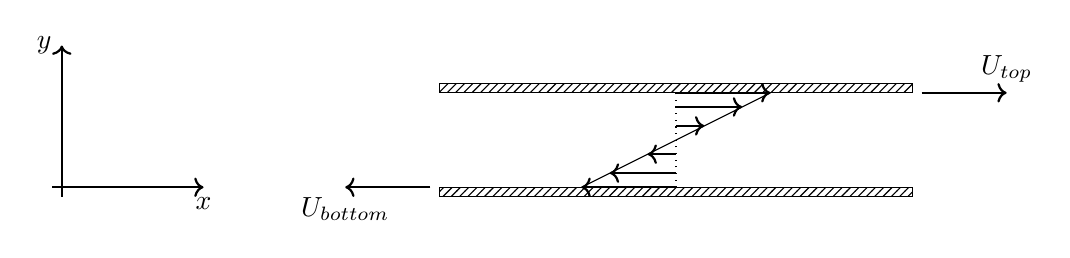
\begin{tikzpicture}[scale=1.2]
 \draw [pattern=north east lines] (0,0) -- (0,-0.1) -- (5,-0.1) -- (5,0) -- cycle;
 \draw [pattern=north east lines] (0,1) -- (0,1.1) -- (5,1.1) -- (5,1) -- cycle;

 \draw [->,thick] (5.1,1)--(6,1) node[above] {$U_{top}$};
 \draw [->,thick] (-0.1,0)--(-1,0) node[below] {$U_{bottom}$};
 
 \draw [->,thick] (-4,-0.1)--(-4,1.5) node[left] {$y$};
 \draw [->,thick] (-4.1,0)--(-2.5,0) node[below] {$x$};
 
 \draw [dotted] (2.5,0.0) to (2.5,1.0);
 \draw  (1.5,0.0) to (3.5,1.0);
 
 \draw [->,thick] (2.5,0.0) to (1.5,0.0);
 \draw [->,thick] (2.5,0.15) to (1.8,0.15);
 \draw [->,thick] (2.5,0.35) to (2.2,0.35);

 \draw [->,thick] (2.5,1) to (3.5,1);
 \draw [->,thick] (2.5,0.85) to (3.2,0.85);
 \draw [->,thick] (2.5,0.65) to (2.8,0.65);
\end{tikzpicture}
\end{center}
\caption{Couette Flow}
\label{couette}
\end{figure}


\noindent
The velocity profile equation is shown below:

\begin{equation}
 u = \big[ U_{top} - U_{bottom} \big] \frac{y}{L} + U_{bottom}
\end{equation}

\medskip
\noindent
where $U_{top}$ is the top plate velocity and its value is
$U_{top} = 1$, 
$U_{bottom}$ is the bottom plate velocity and its value is
$U_{bottom} = -1$, 
$L$ is non-dimensional length
between the plates and its value is $L = 1$
and $y$ is the vertical coordinates and it varies between 
$y = \big[ 0,1 \big]$.
The domaian was discretizes using a linear triangula mesh with 
3835 nodes and 7299 elements. 

\bigskip
The \ref{velocidade couette} shows the unsteady velocity profile
when $Re=100$, in addition to the comparison between 
the numerical solution and the analytical solution 
in the steady state of the proposed problem. 
It is possible to observe that the numerical solution 
converges to the analytical solution when the flow becomes steady.

\begin{figure}[H]
     \centering
     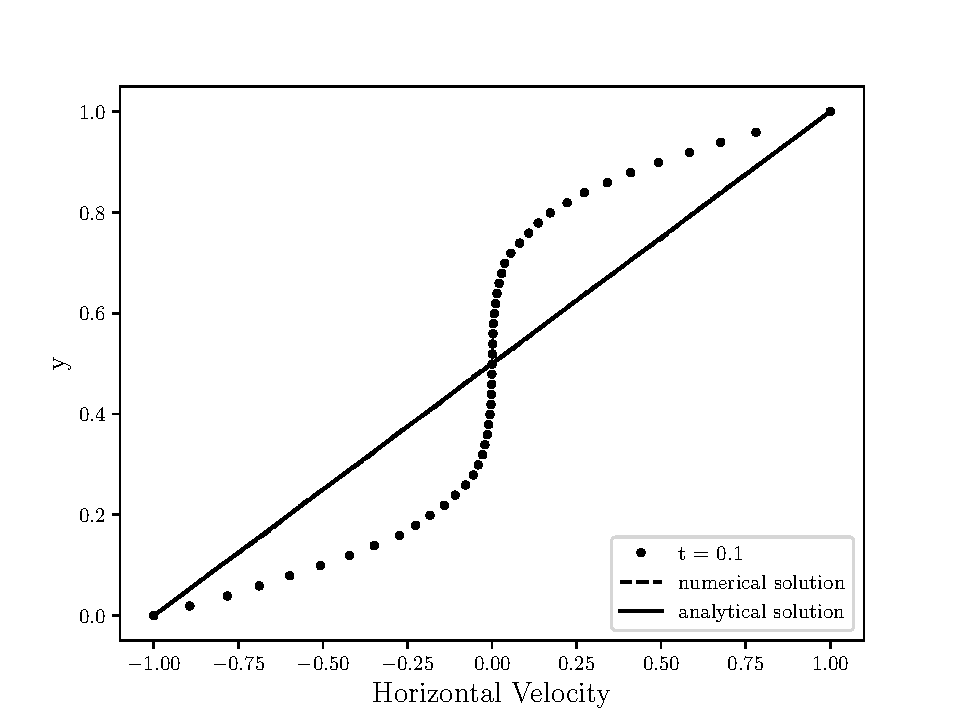
\includegraphics[scale=1]{./02_chaps/cap_validation/figure/couette_velocity.pdf}\\
     \medskip
     \caption{Unsteady velocity profile when $Re=100$ and
     the comparison between the numerical and analytical solution 
     for Couette flow.}
     \label{velocidade couette}
\end{figure}



\section{\textbf{Poiseuille Flow}} 
\label{poiseuille}

A monophase, steady and fully developed flow of a Newtonian 
and incompressible fluid between parallel and fixed horizontal 
plates is maintained due to a pressure gradient 
$\partial p/ \partial x$ imposed as mentioned by Pontes 
and Mangiavacchi (2016) \cite{pontes2016}. 
This flow is known as \textit{Poiseuille flow}. 
The \ref{poiseuille} presents schematically this flow and 
the expected velocity field.

\begin{figure}[H]
\caption{Poiseuille Flow}
\begin{center}
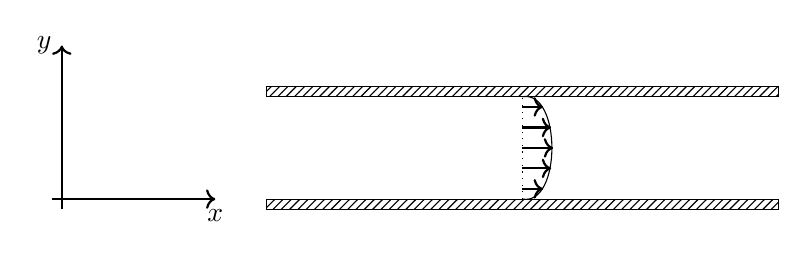
\begin{tikzpicture}[scale=1.3]
 \draw [pattern=north east lines] (0,0) -- (0,-0.1) -- (5,-0.1) -- (5,0) -- cycle;
 \draw [pattern=north east lines] (0,1) -- (0,1.1) -- (5,1.1) -- (5,1) -- cycle;

 \draw [->,thick] (-2,-0.1)--(-2,1.5) node[left] {$y$};
 \draw [->,thick] (-2.1,0)--(-0.5,0) node[below] {$x$};
 
 \draw [dotted] (2.5,0.0) to (2.5,1.0);
 \draw  (2.5,0.0) to [bend right=100] (2.5,1.0);
 
 \draw [->,thick] (2.5,0.9) to (2.7,0.9);
 \draw [->,thick] (2.5,0.7) to (2.78,0.7);
 \draw [->,thick] (2.5,0.5) to (2.8,0.5);
 \draw [->,thick] (2.5,0.3) to (2.78,0.3);
 \draw [->,thick] (2.5,0.1) to (2.7,0.1);
\end{tikzpicture}
\end{center}
\label{poiseuille}
\end{figure}

\noindent
The velocity profile equation is shown below:

\begin{equation}
 u = \frac{4 u_{max}}{L^2} y \big[ L - y \big]
\end{equation}

\medskip
\noindent
where $u_{max}$ is maximum velocity and its value is 
$u_{max} = 1.5$, $L$ is non-dimensional length 
between the plates and its value is 
$L = 1$
and $y$ is the vertical coordinates and it varies 
between $y = \big[ 0,1 \big]$.
The domain was discretized using a linear triangular mesh
with 3835 nodes and 7299 elements.
The \ref{velocidade poiseuille} shows the steady state velocity profile
when $Re=100$.
It is possible to observe that the numerical
solution converges to the analytical solution.

\vspace{1cm}
\begin{figure}[H]
     \caption{
Steady state velocity profile when $Re=100$ and the comparison between
the numerical and analytical solution for Poiseuille flow.} 
     \centering
     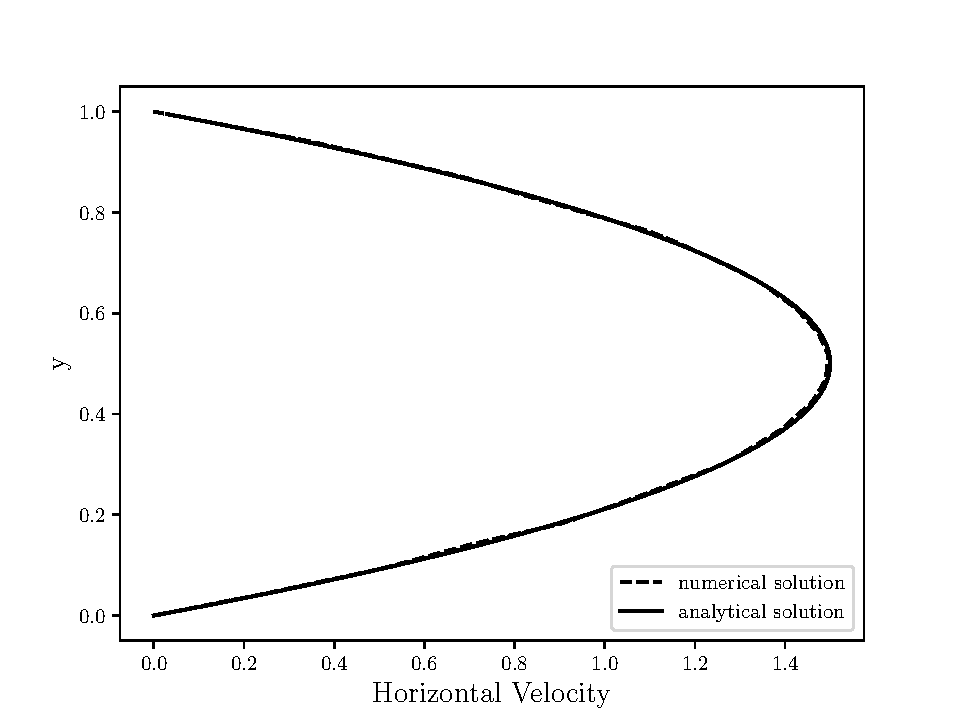
\includegraphics[scale=1]{./02_chaps/cap_validation/figure/poiseuille_velocity.pdf}\\
     \medskip
     \label{velocidade poiseuille}
\end{figure}

\newpage
The \ref{erro relativo poiseuille tabela} shows the relative error 
between the numerical solution and the analytical solution 
for several unstructured linear triangular meshes, ranging 
from 100 to 25600 linear triangular elements. For the mesh 
with 7299 elements as in the case of this benchmark problem, 
the estimated relative error for the velocity field is 0.4\%.

\vspace{0.5cm}
\begin{table}[H]
\caption{The relative error of numerical solution for several elements numbers in an unstructured linear triangular mesh.}
\centering
\begin{tabular}{ccc}
\toprule
\textbf{Elements} & \textbf{Error} (\%) \\
\midrule
100 & 25.00 \\
400 & 7.47 \\
1600 & 2.11 \\
6400 & 0.61 \\
25600 & 0.17 \\
\bottomrule
\end{tabular}
\label{erro relativo poiseuille tabela}
\end{table}

\noindent
\medskip
The relative error was estimated as:

\begin{equation}
 \mathit{Error} = \sqrt{\frac{\sum{(v_{n} - v_{a})^{2} }}{\sum |v_{a}|^{2} }}
\end{equation}

\noindent
where $v_{n}$ is the numerical velocity fielf and
$v_{a}$ is the analytical velocity field.

\bigskip
The \ref{ordem de convergencia poiseuille} presents the relative error 
of the numerical solution with the first and second order convergence 
curves on a log-log scale. As can be seen, the relative error of 
the numerical solution for Poiseuille flow has the form of 
first order convergence. Thus, when increasing the number of elements, 
the relative error of the numerical solution regresses linearly.
A possible cause is due to the vorticity boundary condition used 
in this work. Therefore, the use of the 2a-order boundary condition
would possibly improve the order convergence of the numerical
solution. However, it is necessary to be investigated. 


\begin{figure}[H]
     \caption{Convergence order in log-log scale:
It is estimated the the relative error of numerical solution has
first order convergence.}
     \centering
     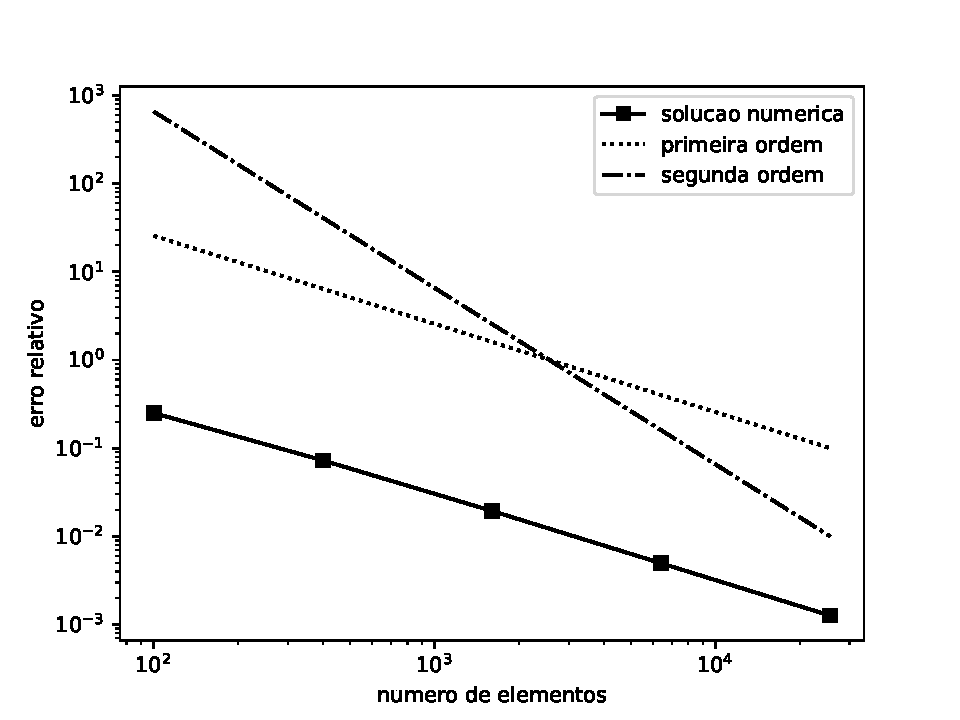
\includegraphics[scale=1]{./02_chaps/cap_validation/figure/poiseuille_error.pdf}\\
     \medskip
     \label{ordem de convergencia poiseuille}
\end{figure}




\section{\textbf{Half Poiseuille Flow}} 
\label{half poiseuille}

Nesta seção é apresentado a simulação do escoamento
de \textit{Poiseuille} na metade do domínio. Dessa forma,
a condição de contorno de superfície livre de escorregamento
é necessária no eixo de simetria.
A \ref{half poiseuille} apresenta esquematicamente este escoamento com o
eixo de simetria especificado e
o perfil do campo de velocidade esperado.

\begin{figure}[H]
\begin{center}
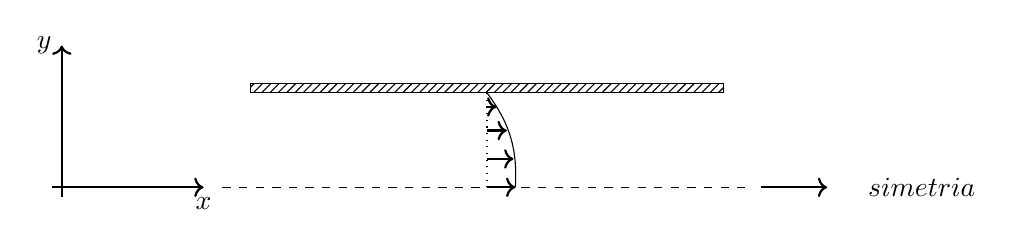
\begin{tikzpicture}[scale=1.2]
 \draw [pattern=north east lines] (0,1) -- (0,1.1) -- (5,1.1) -- (5,1) -- cycle;
 \draw [dashed] (-0.3,0.0) to (5.3,0.0);

 \draw [->,thick] (-2,-0.1)--(-2,1.5) node[left] {$y$};
 \draw [->,thick] (-2.1,0)--(-0.5,0) node[below] {$x$};

 \draw [->,thick] (5.4,0.0)--(6.1,0.0);
 \node [draw=none] at (7.1,0.0) {$simetria$};
 
 \draw [dotted] (2.5,0.0) to (2.5,1.0);
 \draw  (2.8,0.0) to [bend right=20] (2.5,1.0);
 
 \draw [->,thick] (2.5,0.0) to (2.8,0.0);
 \draw [->,thick] (2.5,0.3) to (2.78,0.3);
 \draw [->,thick] (2.5,0.6) to (2.71,0.6);
 \draw [->,thick] (2.5,0.85) to (2.6,0.85);
\end{tikzpicture}
\end{center}
\caption{Escoamento de Poiseuille em Meio Domínio}
\label{half poiseuille}
\end{figure}

\noindent
O perfil de velocidade que este escoamento adquire 
é dado pela equação abaixo:

\begin{equation}
 u = u_{max} \big[ 1 - \frac{y^{2}}{L^{2}} \big]
\end{equation}


\medskip
\noindent
onde $u_{max}$ é a velocidade máxima e seu valor é
$u_{max} = 1.5$, $L$ é a largura não dimensional
entre a placa e o eixo de simetria, seu valor é $L = 1$
e $y$ é a distância entre a placas e o eixo de simetria,
a mesma varia entre $y = \big[ 0,1 \big]$.
O domínio foi discretizado utilizando uma malha 
triangular linear com 3835 nós e 7299 elementos. 

\medskip
\noindent
As condições de contorno utilizadas foram:

\begin{itemize}
     \item \textit{condição de entrada}:
      a componente normal da velocidade $v=0$ enquanto a componente tangencial da velocidade é $u = 1$.                 
      A função de corrente também é especificada e seu valor é definido segundo a equação da continuidade  
      para um fluido incompressível. Dessa forma, seu valor será $\psi = y$.

     \item \textit{condição de não escorregamento}: esta condição é utilizada na placa superior, 
      onde todas as componentes da velocidade são especificadas    
      com os valores $u=0$ e $v=0$.                       
      A função de corrente também é espeficado com o valor $\psi=1$.               
      
     \item \textit{condição de saída}: O valor da função de corrente é especificado $\psi=y$. As derivadas das 
     componentes tangencial e normal da velocidade possuem o 
     valor nulo, isto é,
      $\partial u/\partial n = 0$ e
      $\partial v/\partial n = 0$ respectivamente.   

     \item \textit{condição de livre escorregamento}: esta condição é utilizada no eixo de simetria.
      A componente normal da velocidade e a função de corrente possuem seus valores especificados,
      tais como $v=0$ e $\psi=0$ respectivamente. A derivada da componente tangencial da velocidade
      possuei o valor nulo $\partial u/\partial n = 0$.
\end{itemize}

\medskip
A \ref{velocidade half poiseuille} apresenta a evolução 
do perfil de velocidade no tempo quando o $Re=100$, além do comparativo
entre a solução numérica e a solução analítica no estado permanente do
problema proposto. É possível observar um pequeno desvio entre a solução numérica
e a solução analítica próximo ao eixo de simetria. 

\begin{figure}[H]
     \centering
     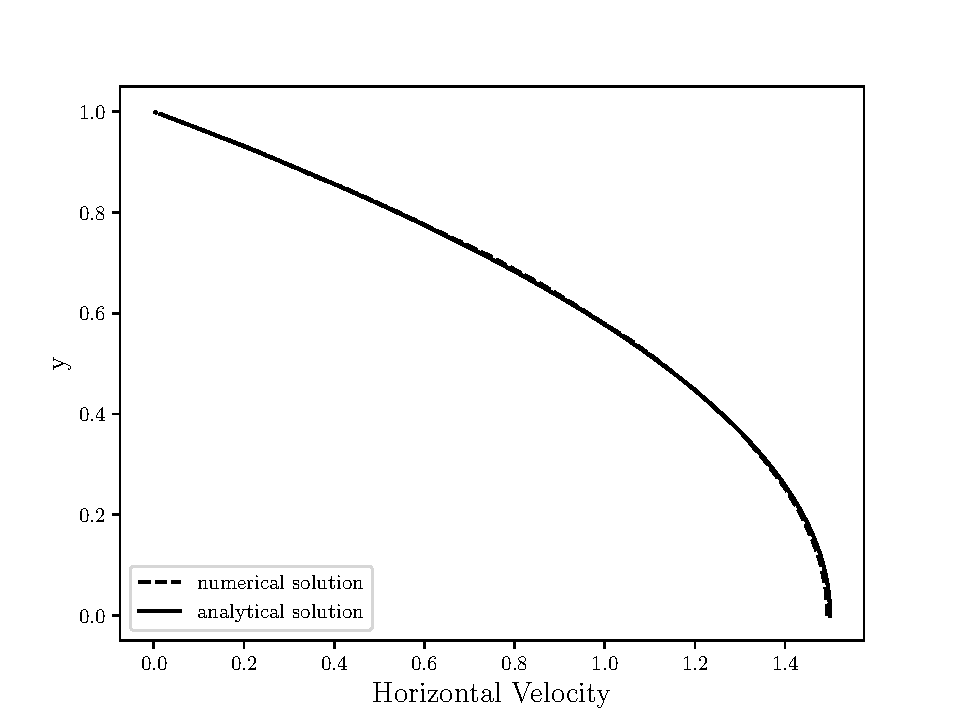
\includegraphics[scale=1]{./02_chaps/cap_validation/figure/half_poiseuille_velocity.pdf}\\
     \medskip
     \caption{Evolução do perfil de velocidade no tempo para $Re=100$ e
     a comparação da solução numérica com a solução analítica para o Escoamento de Poiseuille em Meio Domínio.}
     \label{velocidade half poiseuille}
\end{figure}

\newpage


\section{\textbf{Lid-Driven Cavity}} 
\label{cavity}

A flow in a cavity where the side and bottom walls are fixes and 
the cover moves at a constant velocity such as \textit{$U_{top}=1$} 
is known as \textit {Lid-driven Cavity flow}.
In addition to 
yhe streamfunction is set null value in all boundary, 
because there is no volumetric flux crossing the boundaries 
in lid-driven cavity flow.
The \ref{cavity} presents schematically this flow and 
the expected velocity field.

\vspace{1cm}
\begin{figure}[H]
\caption{Lid-driven Cavity Flow}
\begin{center}
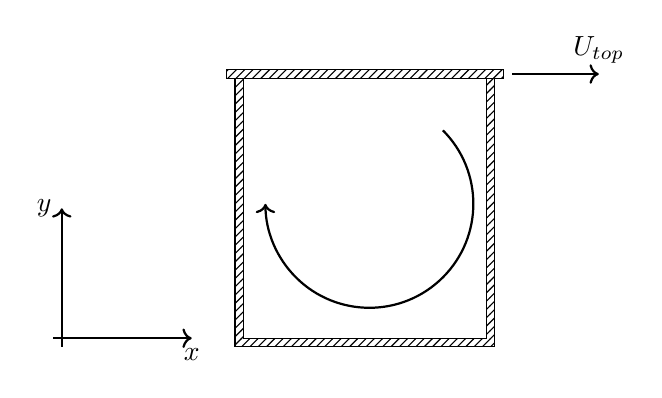
\begin{tikzpicture}[scale=1.1]
 \draw [pattern=north east lines] (0,-0.1) -- (3,-0.1) -- (3,3) -- (2.9,3) -- (2.9,0) -- (0.1,0) -- (0.1,3) -- (0,3) -- cycle;
 \draw [pattern=north east lines] (-0.1,3) -- (-0.1,3.1) -- (3.1,3.1) -- (3.1,3) -- cycle;

 \draw [->,thick] (3.2,3.05)--(4.2,3.05) node[above] {$U_{top}$};

 \draw [->,thick] (2.4,2.4) arc (45:-180:1.2);
 
 \draw [->,thick] (-2,-0.1)--(-2,1.5) node[left] {$y$};
 \draw [->,thick] (-2.1,0)--(-0.5,0) node[below] {$x$};

\end{tikzpicture}
\end{center}
\label{cavity}
\end{figure}

\bigskip
The benchmark problem were simulated with the following 
Reynolds numbers (\textit{Re}): 10, 100, 400 and 1000.
The \ref{velocity vx cavity} and \ref{velocity vy cavity} 
present the profile of the horizontal and vertical velocities,
respectively,
for steady state in several Reynolds number. 
They were compared with 
Ghia et al. (1982) \cite{ghia1982} and 
Marchi et al. (2009) \cite{marchi2009}. 
The domain was discretized using a linear triangular mesh 
with 1563 nodes and 2988 elements.

\begin{center}
\begin{figure}[H]
     \caption{The horizontal velocity profile in central line of cavity ($x=0.5$) for several Reynolds number}
     \centering
     \begin{minipage}{.5\linewidth}
      \centering
      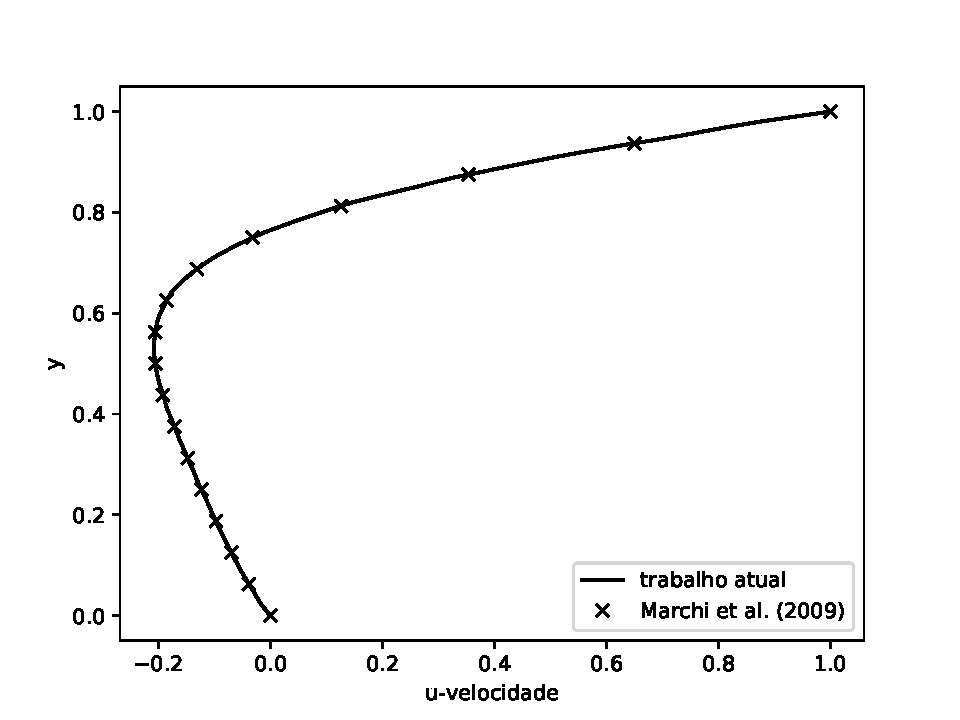
\includegraphics[scale=0.53]{./02_chaps/cap_validation/figure/Re_10_u_profile.pdf}\\
      (a) $Re=10$
     \end{minipage}%
     \begin{minipage}{.5\linewidth}
      \centering
      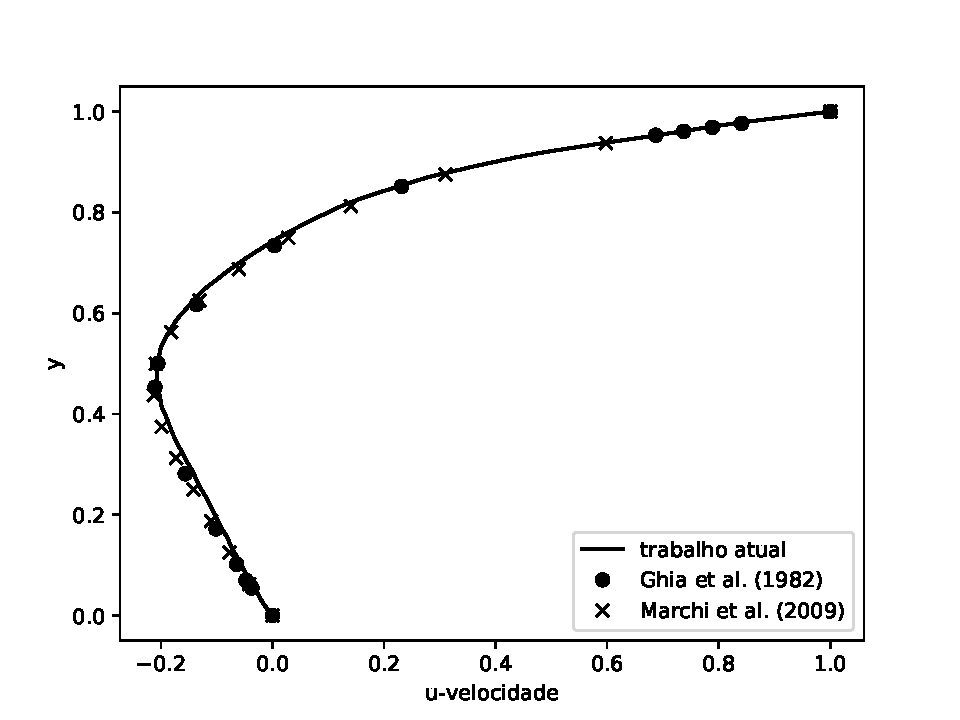
\includegraphics[scale=0.53]{./02_chaps/cap_validation/figure/Re_100_u_profile.pdf}\\
      (b) $Re=100$
     \end{minipage}
     \begin{minipage}{.5\linewidth}
      \centering
      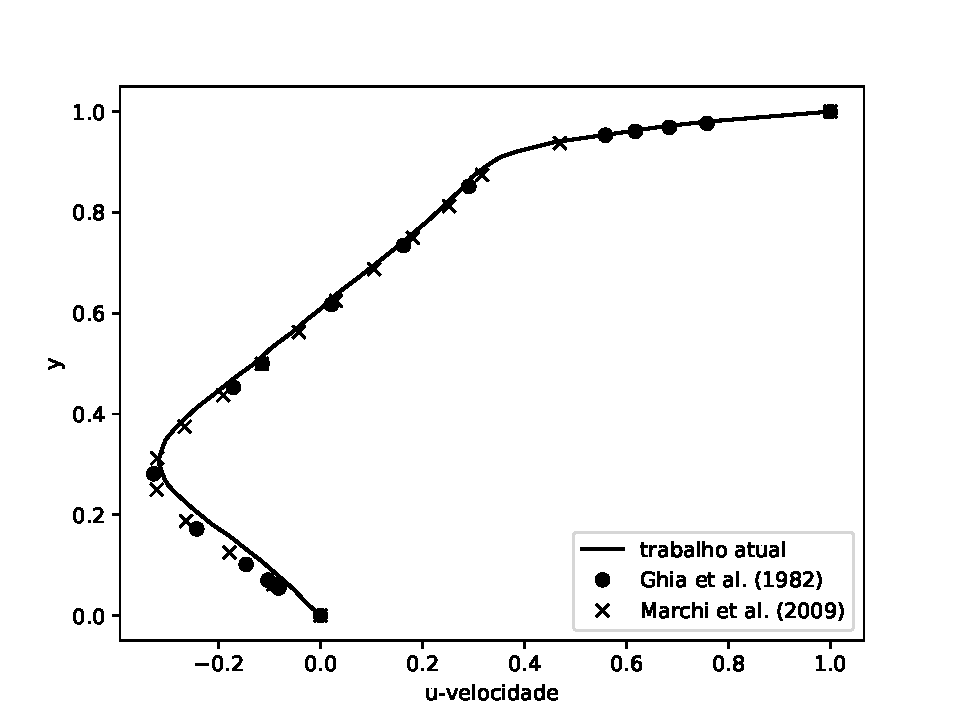
\includegraphics[scale=0.53]{./02_chaps/cap_validation/figure/Re_400_u_profile.pdf}\\
      (c) $Re=400$
     \end{minipage}%
     \begin{minipage}{.5\linewidth}
      \centering
      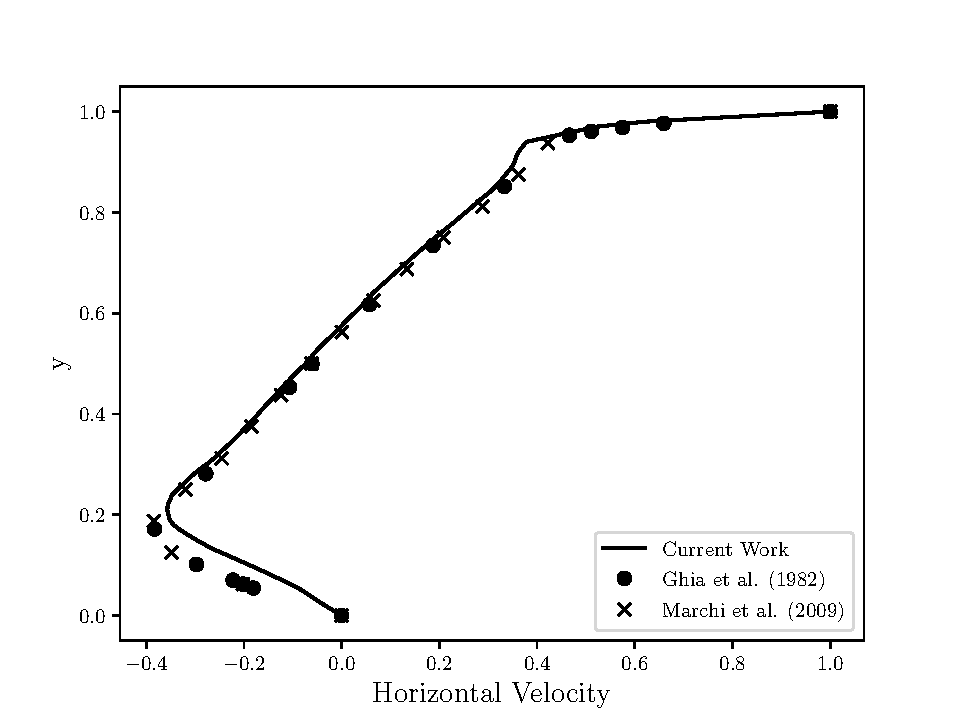
\includegraphics[scale=0.53]{./02_chaps/cap_validation/figure/Re_1000_u_profile.pdf}\\
      (d) $Re=1000$
     \end{minipage}
     \medskip
     \label{velocity vx cavity}
\end{figure}
\end{center}

\begin{figure}[H]
     \caption{The vertical velocity profile in central line of cavity ($y=0.5$) for several Reynolds number}
     \centering
     \begin{minipage}{.5\linewidth}
      \centering
      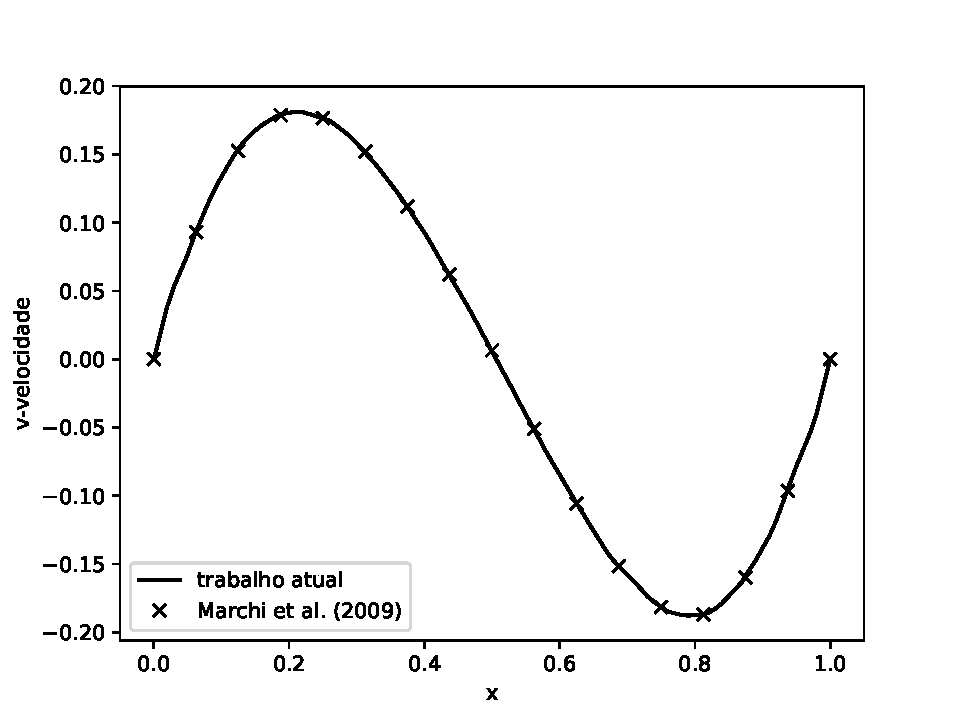
\includegraphics[scale=0.53]{./02_chaps/cap_validation/figure/Re_10_v_profile.pdf}\\
      (a) $Re=10$
     \end{minipage}%
     \begin{minipage}{.5\linewidth}
      \centering
      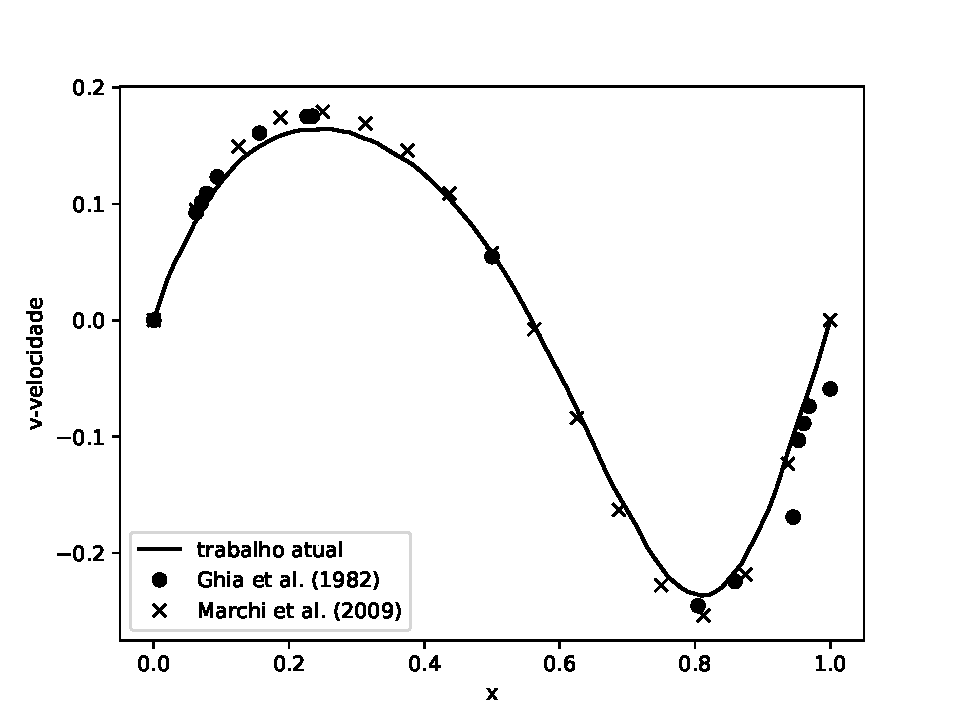
\includegraphics[scale=0.53]{./02_chaps/cap_validation/figure/Re_100_v_profile.pdf}\\
      (b) $Re=100$
     \end{minipage}
     \begin{minipage}{.5\linewidth}
      \centering
      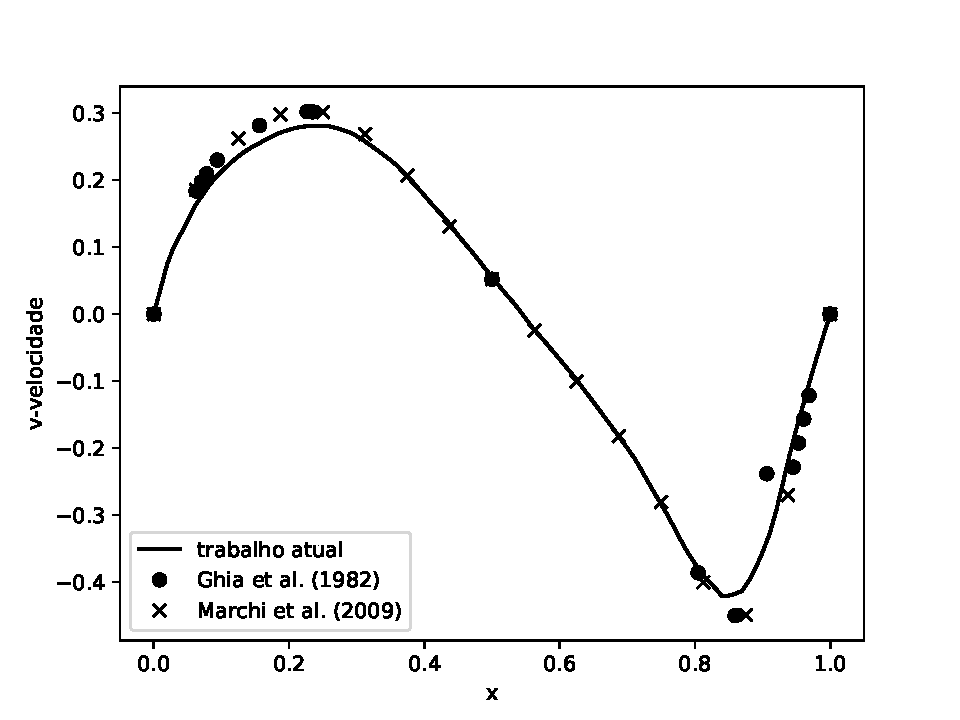
\includegraphics[scale=0.53]{./02_chaps/cap_validation/figure/Re_400_v_profile.pdf}\\
      (c) $Re=400$
     \end{minipage}%
     \begin{minipage}{.5\linewidth}
      \centering
      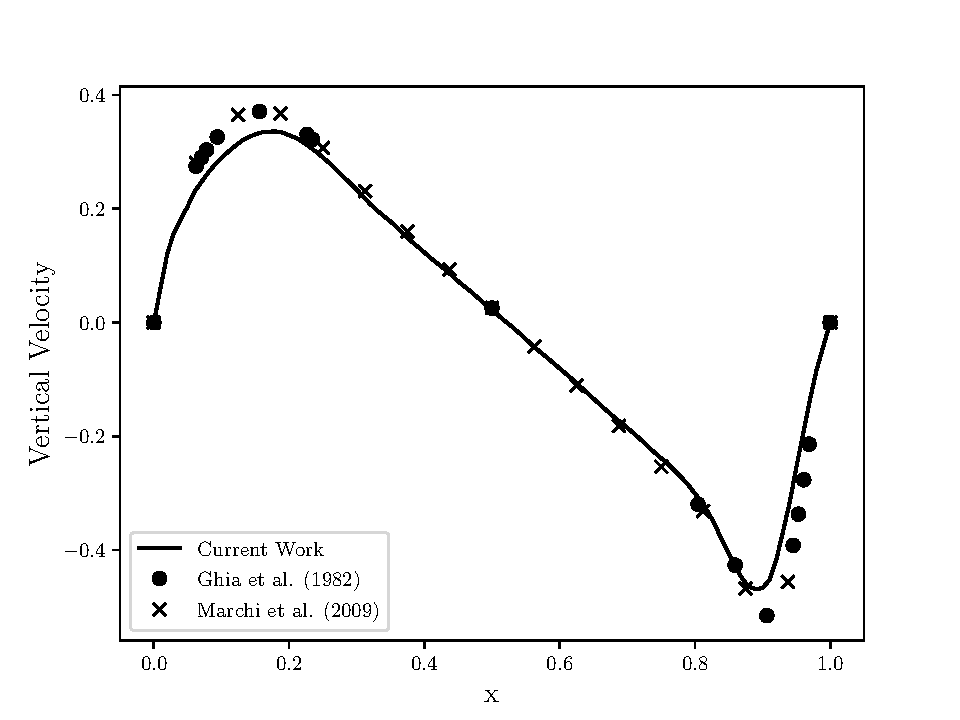
\includegraphics[scale=0.53]{./02_chaps/cap_validation/figure/Re_1000_v_profile.pdf}\\
      (d) $Re=1000$
     \end{minipage}
     \medskip
     \label{velocity vy cavity}
\end{figure}



\section{\textbf{Pure Advection Flow}} 
\label{convection}

The transport of a scalar according to a parabolic function and 
submitted to a monophase flow of a Newtonian and incompressible fluid 
with a high number of \textit{Reynolds} 
($\textit{Re} \rightarrow \infty$) is known as a 
\textit{Pure Advection flow}. In this type of flow, 
it is expected that the scalar will not diffuse. 
For approximation methods like \textit{FEM} and \textit{FDM}, 
it is possible to observe the presence of spurious oscillations. 
As mentioned earlier, several schemes can be used to reduce these 
numerical oscillations. In this section, we will present the use 
of the \textit{semi-Lagrangian} method to reduce spurious oscillations.
In addition, it will be compared to the analytical solution for an
unstructured linear and quadratic triangular mesh 
in order to analyze the numerical diffusion due to the interpolation
as mentioned in the section \ref{discretizacao tempo}. 
The \ref{conveccao} presents schematically the problem and 
the dynamics of scalar transport.

\vspace{0.5cm}
\begin{figure}[H]
\caption{Transport of a scalar in Pure Advection Flow.}
\begin{center}
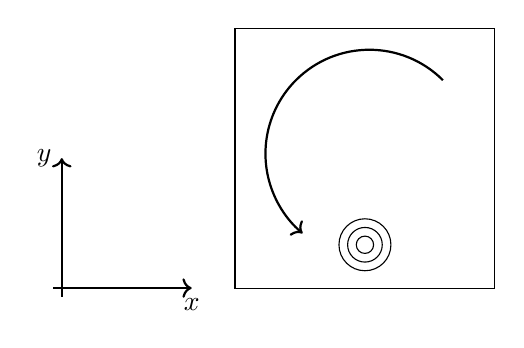
\begin{tikzpicture}[scale=1.1]
 \draw (0,0) -- (3,0) -- (3,3) -- (0,3) -- cycle;

 \draw [->,thick] (2.4,2.4) arc (45:230:1.2);
 
 \draw [->,thick] (-2,-0.1)--(-2,1.5) node[left] {$y$};
 \draw [->,thick] (-2.1,0)--(-0.5,0) node[below] {$x$};

 \draw (1.5,0.5) circle (0.3);
 \draw (1.5,0.5) circle (0.2);
 \draw (1.5,0.5) circle (0.1);

\end{tikzpicture}
\end{center}
\label{conveccao}
\end{figure}

\medskip
\noindent
The scalar transport $\alpha$ for a pure advection flow is shown below:


\begin{equation}
 \frac{\partial \alpha}{\partial t} 
 + 
 \textbf{v} \cdot \nabla \alpha
 = 0
\end{equation}

\noindent
where $\textbf{v} = (u,v)$ is velocity field and its components are
defined as: $u = -y$ e $v = x$. 
Therefore, it is expected that given an initial scalar field, 
it will be displaced by the velocity field without diffusion, 
that is, its profile should not be changed while the flow occurs. 
Any change in the scalar field profile is considered a numerical error.
For this numerical simulation, the domain was discretized using an
unstructured linear triangular mesh with 2216 nodes and 4270 elements
and an unstructured quadratic triangular mesh with 8701 nodes 
and 4270 elements.
In addition to the initial scalar field was defined by a parabolic
profile $c = 1 - x^2 - y^2$, where $x$ and $y$ are space components.



\medskip
The \ref{SL linear} shows the comparison between the scalar field
profile $\alpha$ for the numerical solution using the semi-Lagrangian 
Method in an unstructured linear triangular mesh 
and the analytical solution in 
several positions on the axis of rotation as the flow occurs. 
As can be seen, the spurious oscillations are not observed,
however the scalar field profile in semi-Lagrangian Method
is diffused due to the interpolation. Therefore, for this problem,
the semi-Lagrangian Method in an unstructured linear triangular mesh
did not present a satisfactory result.


\begin{center}
\begin{figure}[H]
     \caption{Comparison of $\alpha$ profile for the semi-Lagrangian Method and analytical solution in several positions on the axis of rotation using an unstructured linear triangular mesh} 
     \centering
     \begin{minipage}{.5\linewidth}
      \centering
      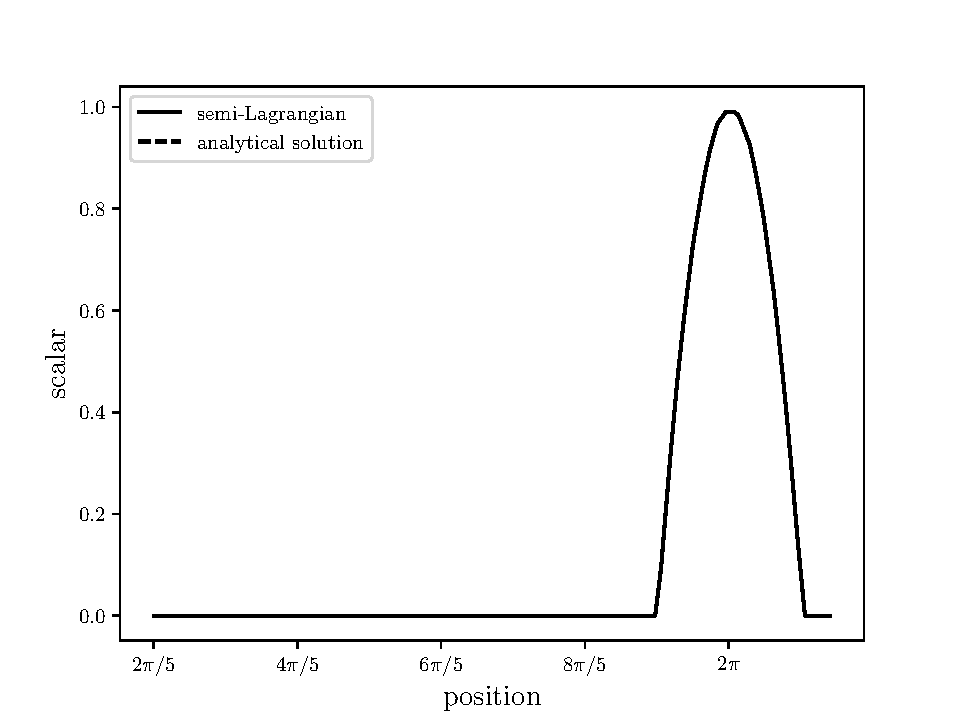
\includegraphics[scale=0.53]{./02_chaps/cap_validation/figure/SLlinear0.pdf}\\
      (a) initial
     \end{minipage}%
     \begin{minipage}{.5\linewidth}
      \centering
      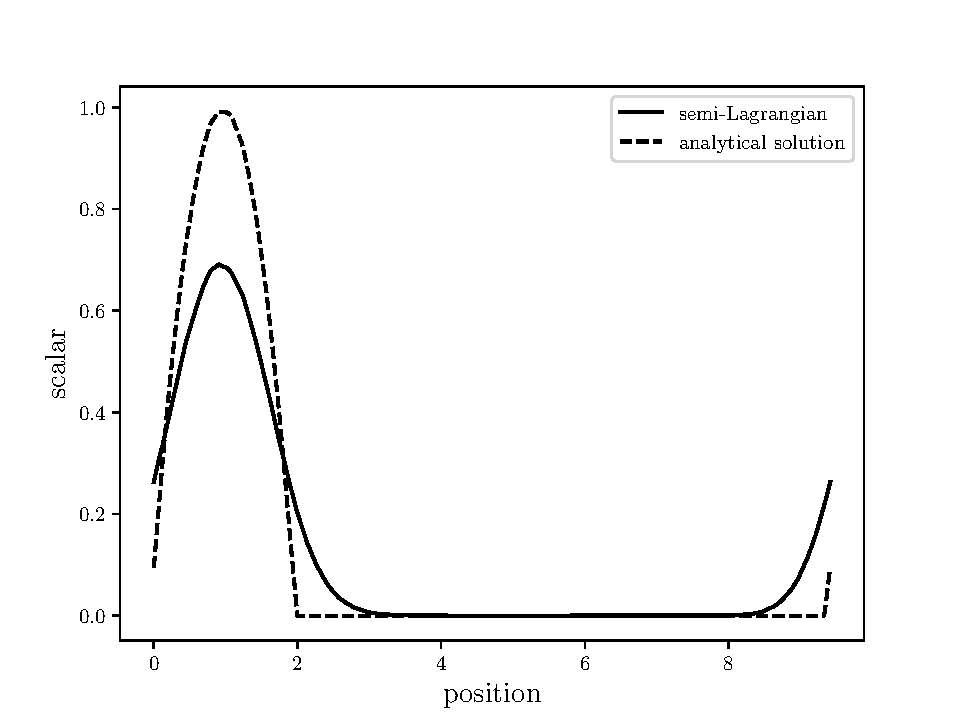
\includegraphics[scale=0.53]{./02_chaps/cap_validation/figure/SLlinear1.pdf}\\
      (b) 1/4 rotation
     \end{minipage}
     \begin{minipage}{.5\linewidth}
      \centering
      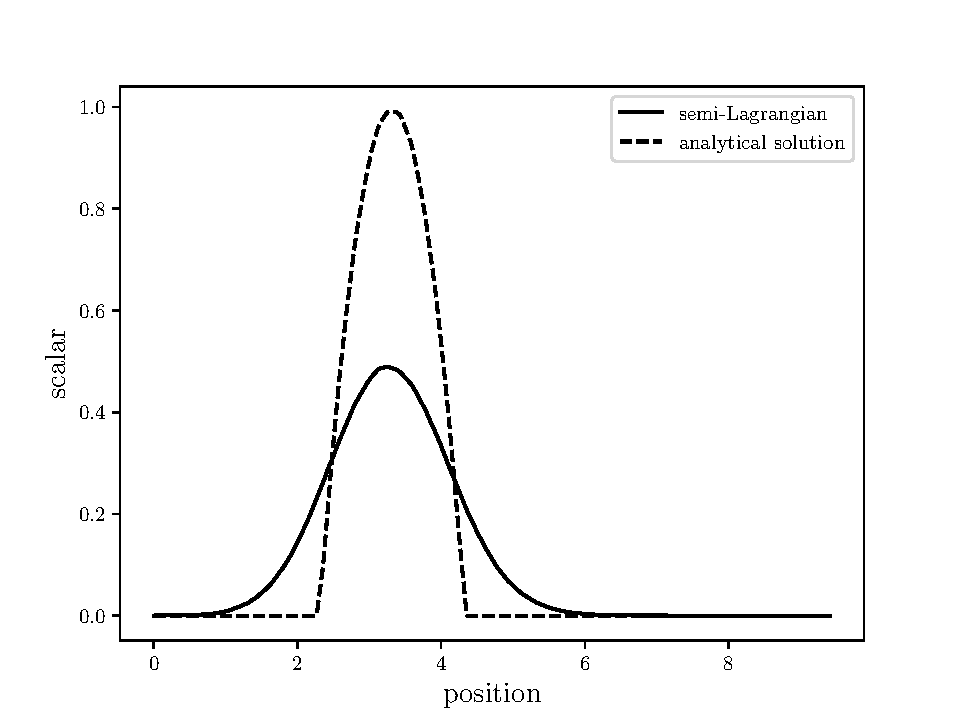
\includegraphics[scale=0.53]{./02_chaps/cap_validation/figure/SLlinear2.pdf}\\
      (c) 1/2 rotation
     \end{minipage}%
     \begin{minipage}{.5\linewidth}
      \centering
      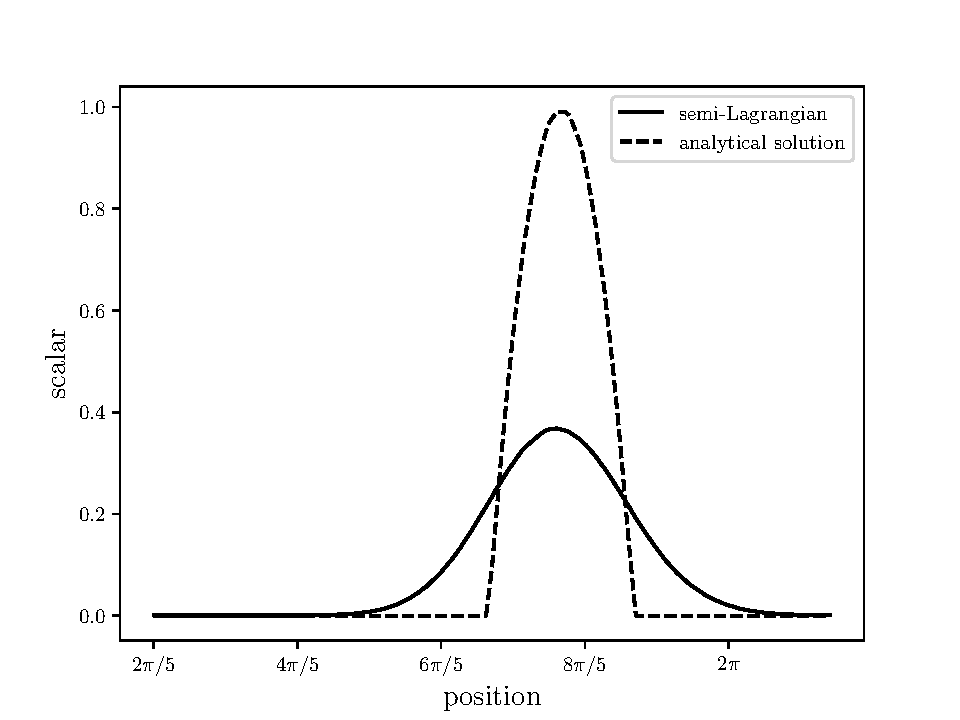
\includegraphics[scale=0.53]{./02_chaps/cap_validation/figure/SLlinear3.pdf}\\
      (d) 3/4 rotation
     \end{minipage}
     \label{SL linear}
\end{figure}
\end{center}


\medskip
The \ref{SL quad} shows the 
comparison between the semi-Lagrangian and analytical solution
for the same previously scalar field
profile $\alpha$,
however an unstructured quadratic triangular mesh is used.
As can be seen, the scalar field profile in semi-Lagrangian Method
shows low numerical diffusion and 
the numerical result is better than the previous one.
In addition, the spurious oscillations are not observed.
Therefore, for this problem,
the semi-Lagrangian Method in an unstructured quadratic triangular mesh
present a satisfactory result.


\begin{center}
\begin{figure}[H]
     \caption{Comparison of $\alpha$ profile for the semi-Lagrangian Method and analytical solution in several positions on the axis of rotation using an unstrutured quadratic triangular mesh} 
     \centering
     \begin{minipage}{.5\linewidth}
      \centering
      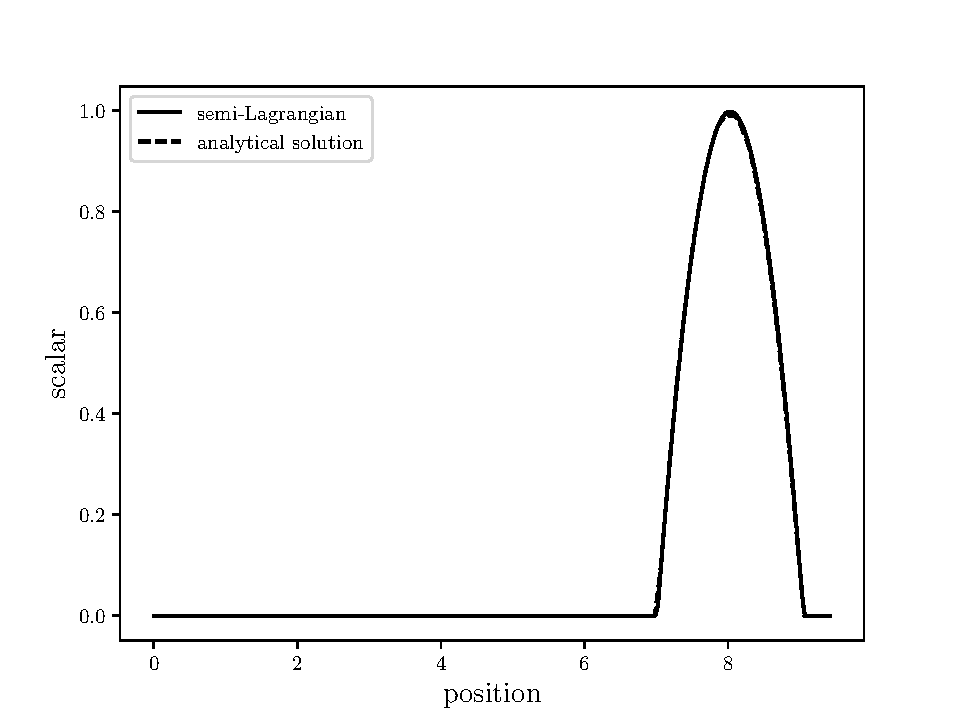
\includegraphics[scale=0.53]{./02_chaps/cap_validation/figure/SLquad0.pdf}\\
      (a) initial
     \end{minipage}%
     \begin{minipage}{.5\linewidth}
      \centering
      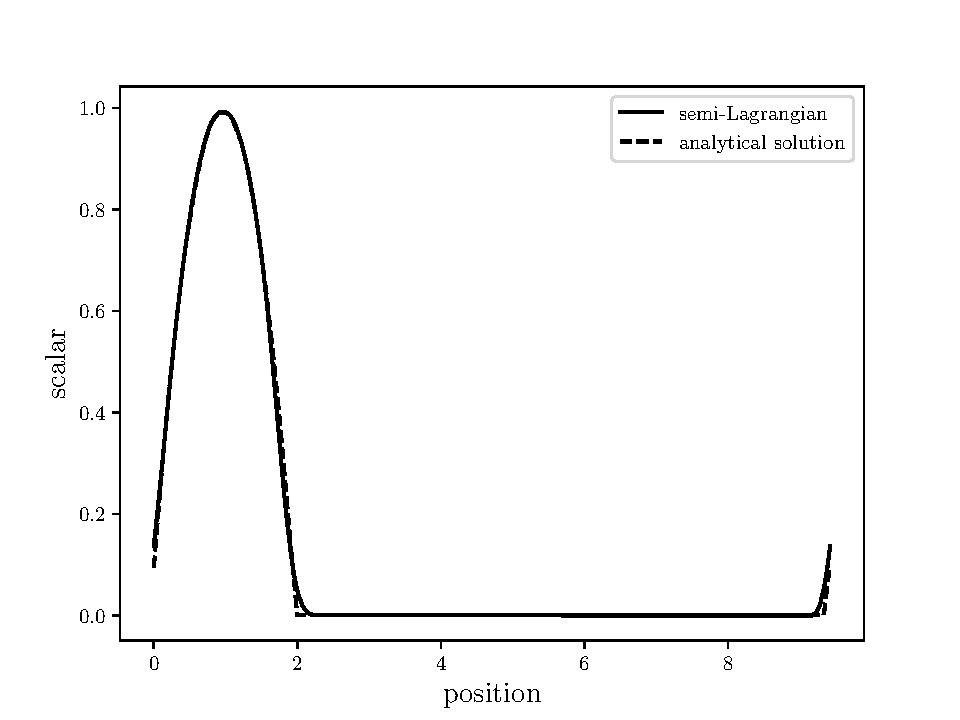
\includegraphics[scale=0.53]{./02_chaps/cap_validation/figure/SLquad1.pdf}\\
      (b) 1/4 rotation
     \end{minipage}
     \begin{minipage}{.5\linewidth}
      \centering
      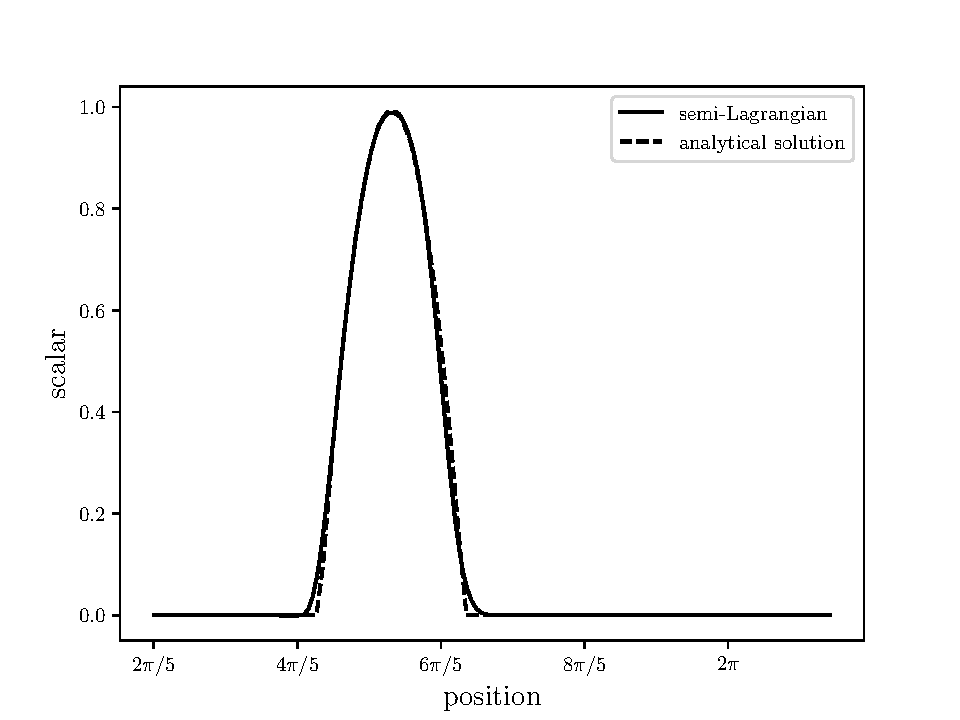
\includegraphics[scale=0.53]{./02_chaps/cap_validation/figure/SLquad2.pdf}\\
      (c) 1/2 rotation
     \end{minipage}%
     \begin{minipage}{.5\linewidth}
      \centering
      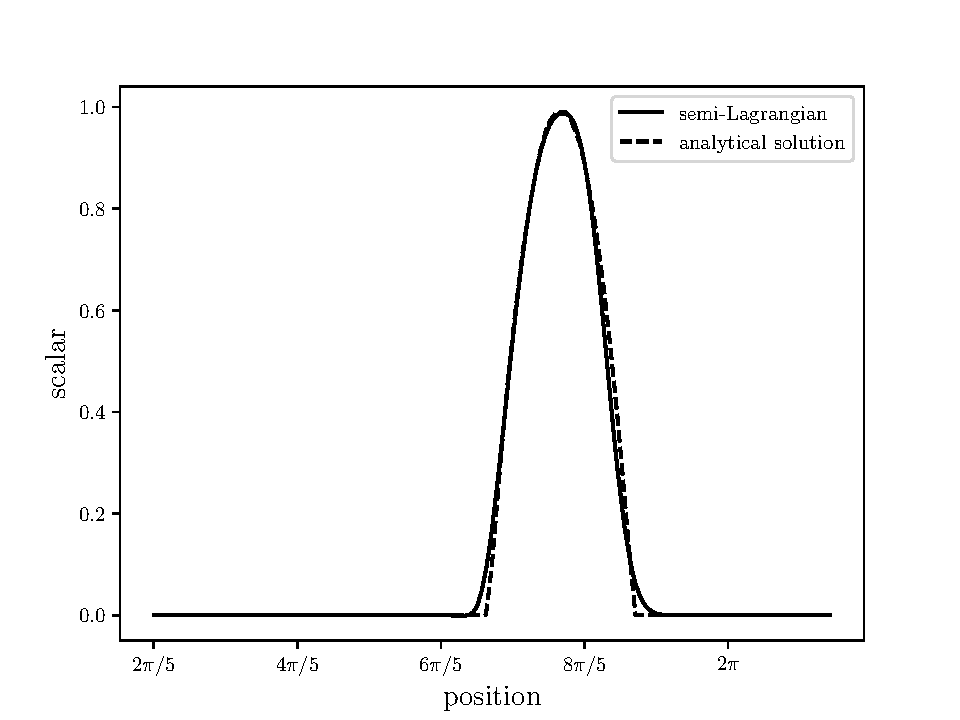
\includegraphics[scale=0.53]{./02_chaps/cap_validation/figure/SLquad3.pdf}\\
      (d) 3/4 rotation
     \end{minipage}
     \label{SL quad}
\end{figure}
\end{center}






\vspace{-1cm}
The \ref{SL linear fig} and \ref{SL quad fig} 
show the spatial and temporal evolution
of the scalar profile for the semi-Lagrangian Method in an
unstructured linear and quadratic triangular mesh  
respectively. As mentioned earlier, the spurious oscillations 
are not presented in both simulations. 
However, in the \ref{SL linear fig}, it is possible
to observe the numerical diffusion, making its use not
recommended for high Reynolds number problem.

\vspace{0.5cm}
\begin{figure}[H]
     \caption{
Spatial and temporal evolution for the semi-Lagrangian Method in several positions of the axis of rotation using an unstructured linear triangular mesh}	
     \centering
     \begin{minipage}{.5\linewidth}
      \centering
      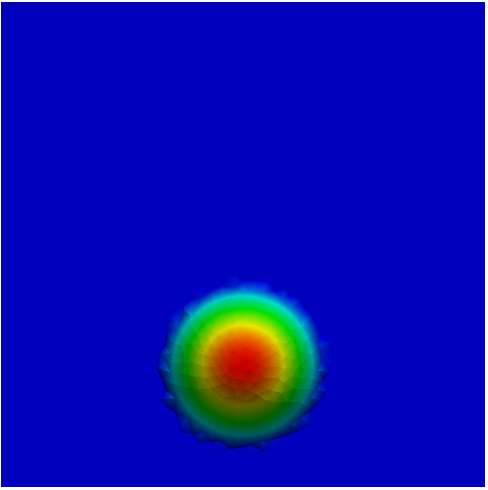
\includegraphics[scale=0.42]{./02_chaps/cap_validation/figure/figSLlinear0.png}\\
      (a) inital
     \end{minipage}%
     \begin{minipage}{.5\linewidth}
      \centering
      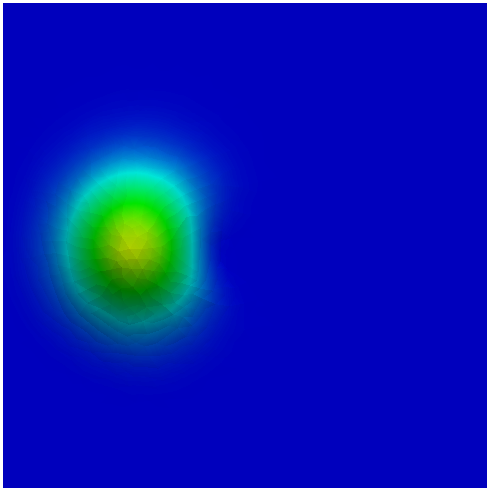
\includegraphics[scale=0.42]{./02_chaps/cap_validation/figure/figSLlinear1.png}\\
      (b) 1/4 rotation
     \end{minipage}\\[10pt]
     \begin{minipage}{.5\linewidth}
      \centering
      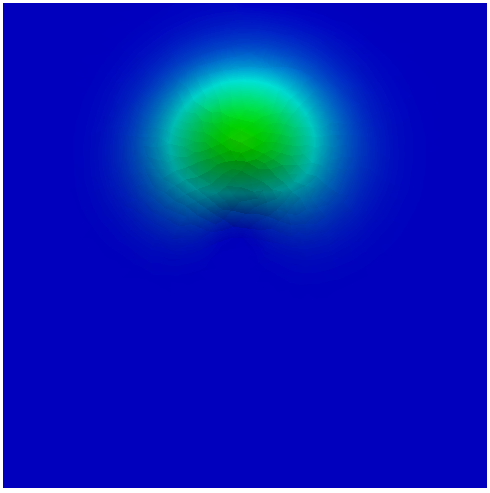
\includegraphics[scale=0.42]{./02_chaps/cap_validation/figure/figSLlinear2.png}\\
      (c) 1/2 rotation
     \end{minipage}%
     \begin{minipage}{.5\linewidth}
      \centering
      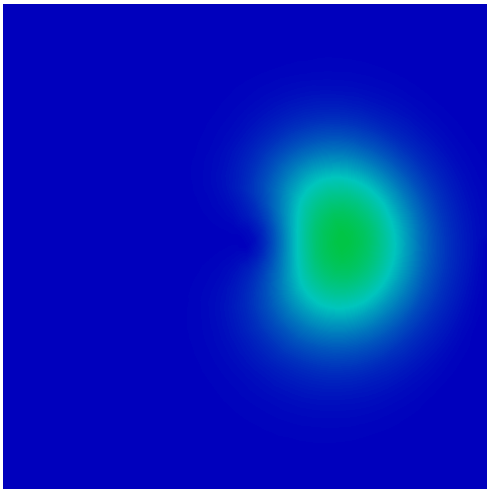
\includegraphics[scale=0.42]{./02_chaps/cap_validation/figure/figSLlinear3.png}\\
      (d) 3/4 rotation
     \end{minipage}
     \label{SL linear fig}
\end{figure}


\vspace{0.5cm}
\begin{figure}[H]
     \caption{
Spatial and temporal evolution for the semi-Lagrangian Method in several positions of the axis of rotation using an unstructured quadratic triangular mesh}	
     \centering
     \begin{minipage}{.5\linewidth}
      \centering
      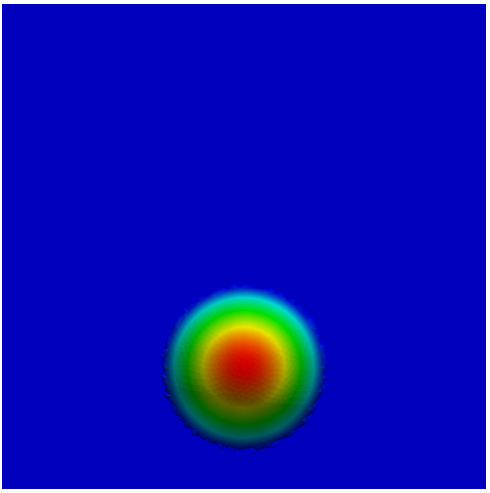
\includegraphics[scale=0.42]{./02_chaps/cap_validation/figure/figSLquad0.png}\\
      (a) initial
     \end{minipage}%
     \begin{minipage}{.5\linewidth}
      \centering
      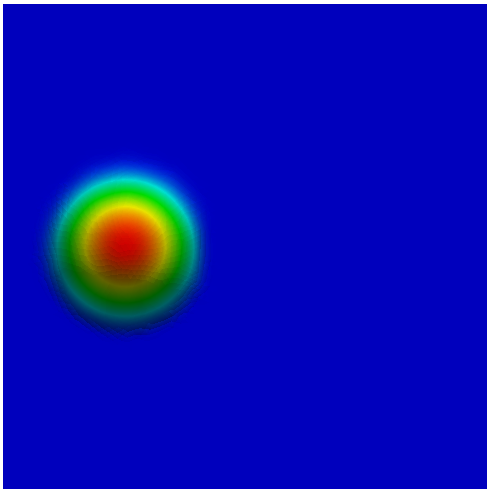
\includegraphics[scale=0.42]{./02_chaps/cap_validation/figure/figSLquad1.png}\\
      (b) 1/4 rotation
     \end{minipage}\\[10pt]
     \begin{minipage}{.5\linewidth}
      \centering
      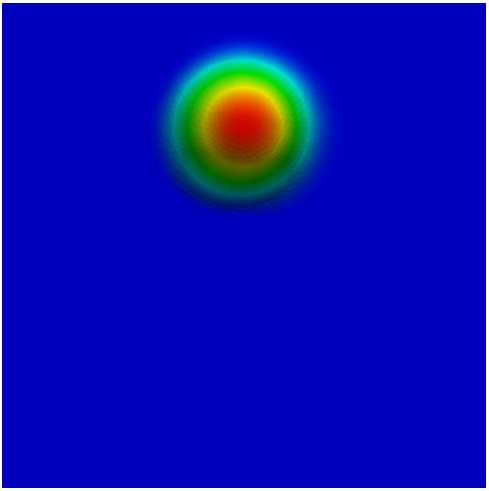
\includegraphics[scale=0.42]{./02_chaps/cap_validation/figure/figSLquad2.png}\\
      (c) 1/2 rotation
     \end{minipage}%
     \begin{minipage}{.5\linewidth}
      \centering
      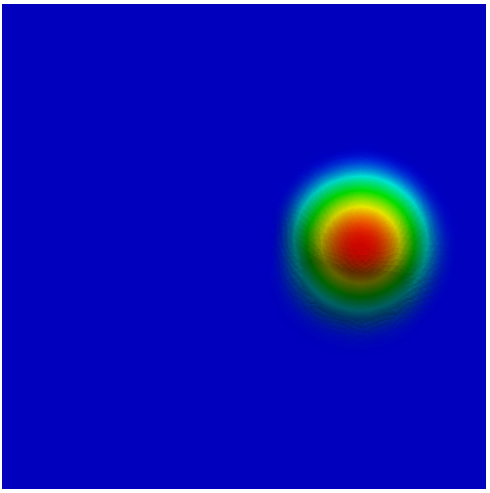
\includegraphics[scale=0.42]{./02_chaps/cap_validation/figure/figSLquad3.png}\\
      (d) 3/4 rotation
     \end{minipage}
     \label{SL quad fig}
\end{figure}




\chapter{\textbf{RESULTS}}
\label{resultados}

\section{\textbf{Introduction}} 
In this chapter, the results of numerical simulations for 
blood flow in a coronary artery are presented. 
The lumen radius of the coronary artery used was $R=0.0015m$, 
the viscosity used was $\mu=0.0035Pa.s$ and the specific gravity used was
$\rho=1060kg/m^3$ as suggested by Bozsak, Chomaz and Barakat (2014)
 \cite{bozsak2014}. According to Kessler et al. (1998) 
\cite{kessler1998}, the blood velocity in the coronary artery 
is $u=12cm/s$. Thus, the Reynolds number used will be 
$Re=54.5$. 

\medskip
The Navier-Stokes equation is used according to the 
vorticity-streamfunction formulation with 
the species transport equation for two geometries proposed 
by Wang et al. (2017) \cite{wang2017}, however modified to 
cartesian coordinates as shown in \ref{coronary artery geo}. 
In the section \ref{canal curvado com stent}, the numerical 
simulation for the coronary artery with atherosclerosis 
and a drug-eluting stent in a curved channel model 
is presented for several 
\textit{Schmidt} number, such as $Sc=1$ and $10$. 
In the \ref{canal real com stent}, the real coronary 
artery with atherosclerosis and a drug-eluting stent is also 
simulated with several numbers of \textit{Schmidt} number 
as in the previous section.
Due to symmetry, only half of the domain is shown. 
The simulation was visualized using the \textit{Paraview} open-source 
software proposed by Henderson (2007) \cite{paraview}.


\begin{figure}[H]
     \centering
     \begin{minipage}{.45\linewidth}
      \centering
      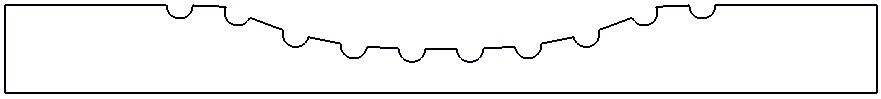
\includegraphics[scale=0.22]{./02_chaps/cap_solution/figure/CurvedStrut.png}\\
      (a)
     \end{minipage}%
     \begin{minipage}{.45\linewidth}
      \centering
      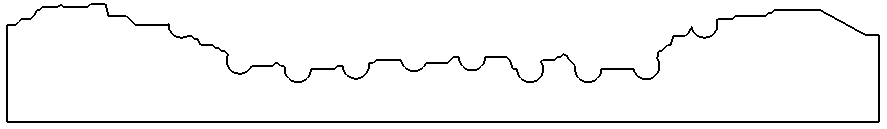
\includegraphics[scale=0.22]{./02_chaps/cap_solution/figure/RealStrut.png}\\
      (b)
     \end{minipage}
     \medskip
     \caption{Non-dimensional domain for the blood flow in coronary artery
     The radius used was $R=1$ and and the lumen length was $L=10R$.
     (a) Curved Channel with Drug-Eluting Stent
     (b) Real Channel with Drug-Eluting Stent.}
     \label{coronary artery geo}
\end{figure}


\section{\textbf{Curved Channel}} 
\label{canal curvado}
Para o caso onde a artéria coronária possui aterosclerose,
o problema é modelado como um escoamento entre placas retas e paralelas
e curvadas. A geometria utilizada promove uma redução suave
da distância entre as paredes superior e inferior do canal.
Foi considerado 40\% de obstrução do canal devido a aterosclerose e
o domínio foi discretizado com 10261 nós e 23049 elementos triangulares lineares. \par
A \ref{velocity evolution curved} apresenta o perfil
de velocidade transiente ao longo da coordenada $y$ no
meio do canal ($x=5R$).
Como podemos observar, 
o valor adimensional máximo do campo de velocidade
chega a $u=2.3$ quando a artéria possui aterosclerose, isto é,
há um aumento de $53$\% da velocidade máxima quando comparado com
a artéria sem aterosclerose como apresentado na \ref{velocidade half poiseuille}.



\begin{figure}[H]
     \centering
     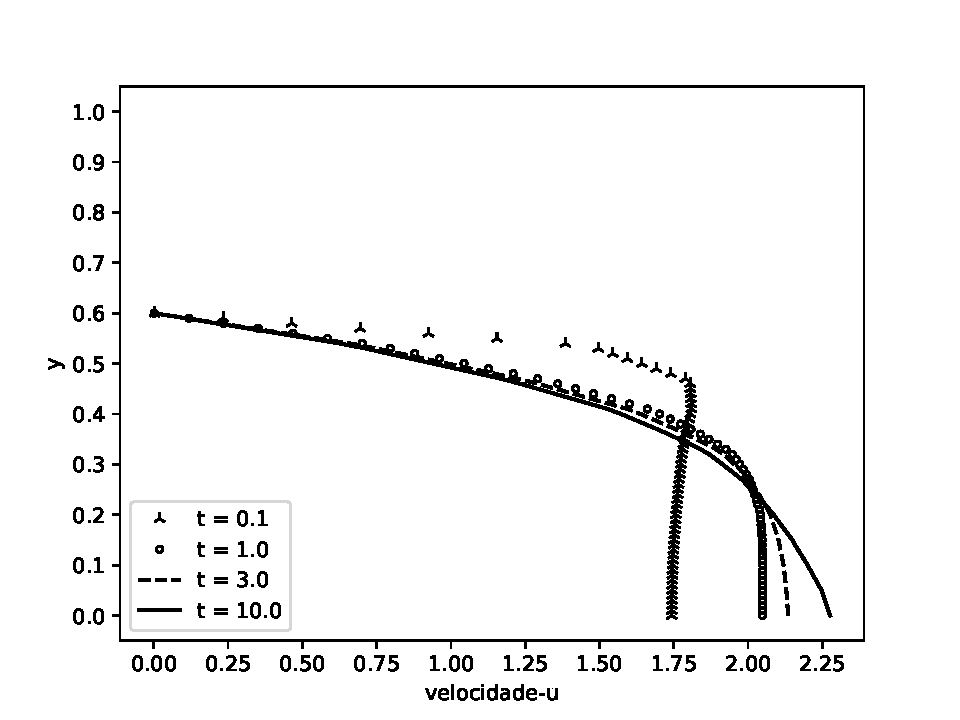
\includegraphics[scale=1]{./02_chaps/cap_solution/figure/vel_Curved_evol.pdf}\\
     \caption{Evolução no tempo do perfil da velocidade para o Canal Curvado.}
     \label{velocity evolution curved}
\end{figure}

\newpage
A \ref{velocity field curved} apresenta a evolução no tempo e no espaço
do campo de velocidade para a metade do domínio, pois os resultados são simétricos
na direção $y$. O campo de velocidade é representado com os valores adimensionais
onde a cor vermelha se refere ao valor $u=2.3$ e a cor azul $u=0$. Transformando em
valores dimensionais temos $u=27.6 cm/s$ e $u=0 cm/s$ respectivamente.

\vspace{2cm} 
\begin{figure}[H]
     \begin{minipage}{.50\linewidth}
      \centering
      
\includegraphics[scale=0.175]{./02_chaps/cap_solution/figure/vel_Curved200.png}\\
      t = 0.1
     \end{minipage}%
     \begin{minipage}{.50\linewidth}
      \centering
      
\includegraphics[scale=0.172]{./02_chaps/cap_solution/figure/vel_Curved1000.png}\\
      t = 0.5
     \end{minipage}
     \begin{minipage}{.50\linewidth}
     \medskip
      \centering
      
\includegraphics[scale=0.175]{./02_chaps/cap_solution/figure/vel_Curved2000.png}\\
      t = 1.0
     \end{minipage}%
     \begin{minipage}{.50\linewidth}
     \medskip
      \centering
      
\includegraphics[scale=0.175]{./02_chaps/cap_solution/figure/vel_Curved6000.png}\\
      t = 3.0
     \end{minipage}
     \begin{minipage}{.50\linewidth}
      \centering
      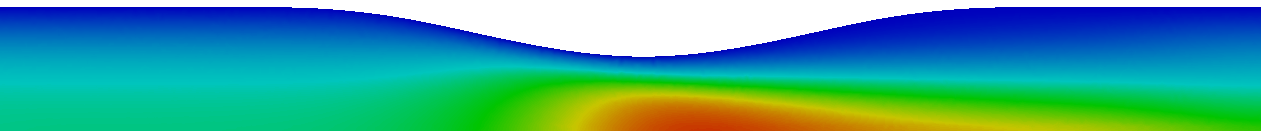
\includegraphics[scale=0.175]{./02_chaps/cap_solution/figure/vel_Curved8000.png}\\
      t = 4.0
     \end{minipage}%
     \begin{minipage}{.50\linewidth}
      \centering
      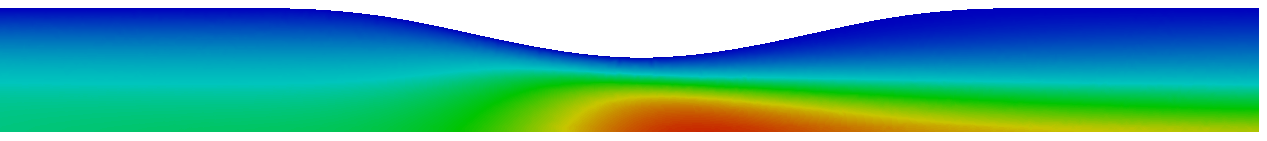
\includegraphics[scale=0.175]{./02_chaps/cap_solution/figure/vel_Curved10000.png}\\
      t = 5.0
     \end{minipage}
     \begin{minipage}{.50\linewidth}
     \medskip
      \centering
      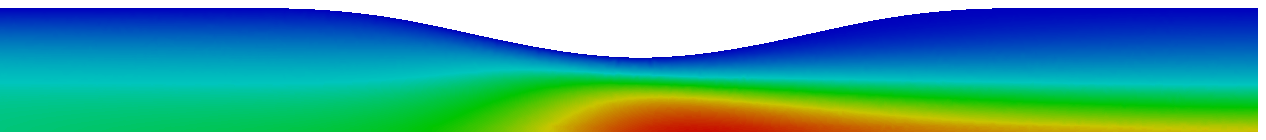
\includegraphics[scale=0.175]{./02_chaps/cap_solution/figure/vel_Curved14000.png}\\
      t = 7.0
     \end{minipage}%
     \begin{minipage}{.50\linewidth}
     \medskip
      \centering
      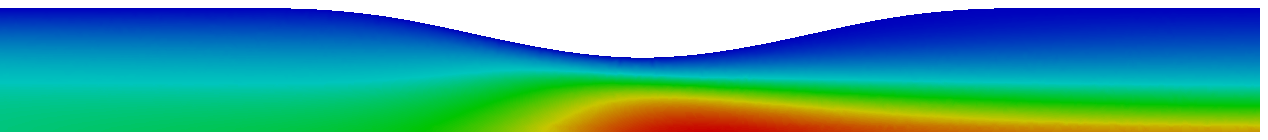
\includegraphics[scale=0.175]{./02_chaps/cap_solution/figure/vel_Curved20000.png}\\
      t = 10.0
     \end{minipage}
     \medskip
     \caption{Evolução no tempo e no espaço do campo de velocidade para o Canal Curvado.}
     \label{velocity field curved}
\end{figure}

\newpage


\section{\textbf{Curved Channel with Drug-Eluting Stent}} 
\label{canal curvado com stent}
In this section, will be present
the case where the coronary 
artery has atherosclerosis and 
the drug-eluting stent is placed. 
It is modeled by 10 uniformly spaced 
semi-circles. 
The geometry used promotes a smooth reduction of the 
distance between the upper wall and symmetry axis of the channel. 
Due to atherosclerosis, 40\% channel obstruction was considered 
and the domain was discretized using 15875 nodes and 35408 
linear triangular elements. 

\medskip 
The \ref{velocity evolution curved stent} shows the unsteady state 
velocity profile in the middle section channel, that is, 
$x=5.0R$. 
As expected, the numerical solution tends to a similar profile to
the Half Poiseuille, as presented in the section \ref{half poiseuille sec}. However, it is possible to observe an inversion of the velocity
field sense at the top of the figure.
This inversion occurs in the region that is
located between the stents strut semi-circles.
It is also possible to observe that the maximum horizontal velocity field 
in curvel channel reaches the $u=3.43$ non-dimensional value, that is, 
more than 3 times the blood velocity in coronary artery
without atherosclerosis and stent strut placed. 
This increase can influence the dynamics of blood flow
and its biological processes and a more detailed analysis
should be performed.

\vspace{1cm}
\begin{figure}[H]
     \caption{
The unsteady state velocity profile in the middle ($x=5.0R$) of the curved channel with drug-eluting stent.}
     \centering
     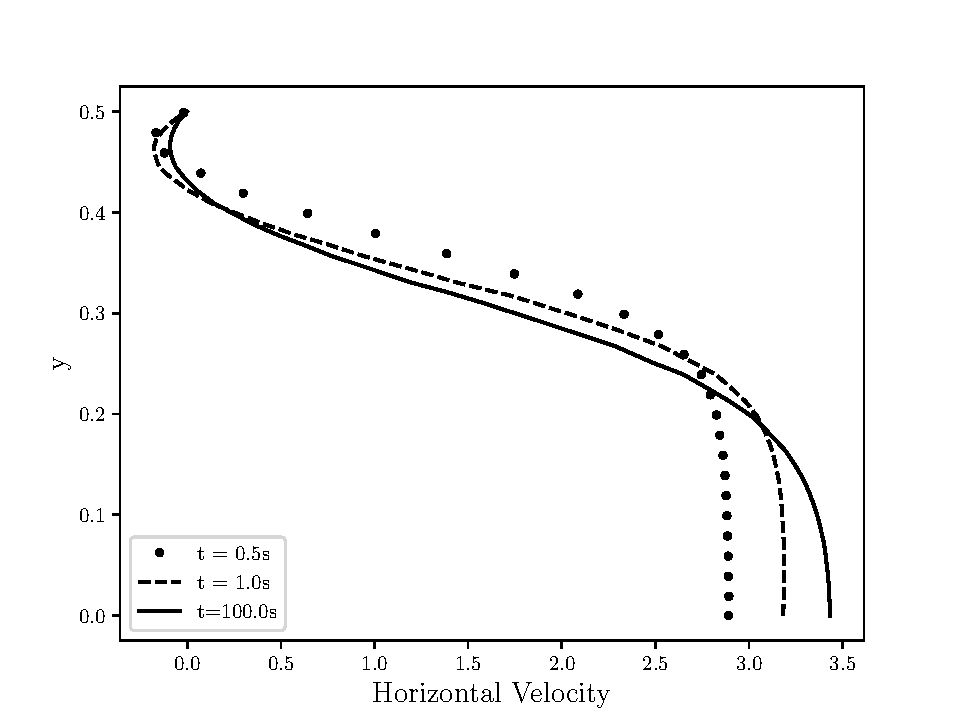
\includegraphics[scale=1]{./02_chaps/cap_solution/figure/vel_CurvedStrut_evol.pdf}\\
     \label{velocity evolution curved stent}
\end{figure}

\newpage
The \ref{velocity field curved stent} presents the evolution in 
time and space of the velocity field for half of the domain
due to the symmetry of the solution. 
The velocity field is represented with non-dimensional values 
where the red color refers to the $u=3.43$ value and the blue color 
$u=0$ value. Conveting to dimensional values, 
we have $u=41.16cm/s$ and $u=0cm/s$ respectively.
As can be seen, the region with the lowest horizontal velocity 
magnitude is found close to the boundary where the no-slip
condition is applied. Whereas, it is increase close to 
the symmetric axis. Moreover, the largest horizontal velocity value
is found in the maximum contraction region.


\vspace{1cm} 
\begin{figure}[H]
     \caption{
Temporal and spatial evolution of the velocity field for curved channel with
drug-eluting stent.}
     \begin{minipage}{.50\linewidth}
      \centering
      \includegraphics[scale=0.18]{./02_chaps/cap_solution/figure/vel_CurvedStrut1.png}\\
      t = 0.1s
     \end{minipage}%
     \begin{minipage}{.50\linewidth}
      \centering
      \includegraphics[scale=0.18]{./02_chaps/cap_solution/figure/vel_CurvedStrut2.png}\\
      t = 0.5s
     \end{minipage}
     \begin{minipage}{.50\linewidth}
     \medskip
      \centering
      \includegraphics[scale=0.18]{./02_chaps/cap_solution/figure/vel_CurvedStrut3.png}\\
      t = 1.0s
     \end{minipage}%
     \begin{minipage}{.50\linewidth}
     \medskip
      \centering
      \includegraphics[scale=0.18]{./02_chaps/cap_solution/figure/vel_CurvedStrut4.png}\\
      t = 3.0s
     \end{minipage}
     \begin{minipage}{.50\linewidth}
      \centering
      \includegraphics[scale=0.18]{./02_chaps/cap_solution/figure/vel_CurvedStrut5.png}\\
      t = 5.0s
     \end{minipage}%
     \begin{minipage}{.50\linewidth}
      \centering
      \includegraphics[scale=0.18]{./02_chaps/cap_solution/figure/vel_CurvedStrut6.png}\\
      t = 7.0s
     \end{minipage}
     \begin{minipage}{.50\linewidth}
     \medskip
      \centering
      \includegraphics[scale=0.18]{./02_chaps/cap_solution/figure/vel_CurvedStrut7.png}\\
      t = 10.0s
     \end{minipage}%
     \begin{minipage}{.50\linewidth}
     \medskip
      \centering
      \includegraphics[scale=0.18]{./02_chaps/cap_solution/figure/vel_CurvedStrut8.png}\\
      t = 100.0s
     \end{minipage}\\[10pt]
      \centering
      \includegraphics[scale=0.5]{./02_chaps/cap_solution/figure/vel_CurvedStrutScale.png}\\
     \medskip
     \label{velocity field curved stent}
\end{figure}


\vspace{1cm}
As mentioned by Lucena et al. (2018) \cite{lucena2018}, 
it is estimated that 47\% of the drug is diffused to the 
lumem and it is lost to the bloodstream.
The \ref{conc field curved stent sc 1} to 
\ref{conc field curved stent sc 1000} show the temporal and spatial evolution 
of the concentration field for several \textit{Schmidt} number, 
such as: $1$, $10$, $100$ and $1000$ respectively. The concentration field is 
represented with the non-dimensional values where the red color 
represents $100$\% and the blue color represents $0$\% 
of the diffused concentration in the bloodstream. 

\medskip
It is possible to observe in the \ref{conc field curved stent sc 1}
that the concentration field is significally more diffuse than in the
\ref{conc field curved stent sc 10}, where the Schmidt number
is 10 times higher. This means that a large portion of the
diffused drug in bloodstream is quickly spread in the
$Sc=1$ case.
Moreover, in both cases, the concentration field
is more dispersed at the end of the curved channel due to
the sense of the blood flow. It is possible that the
drug concentration diffused affects the density and viscosity of the blood
and consequently the Reynolds number. Thefore, the velocity field would
also be affected. However, this influence is not considered in this work.


\vspace{1cm}
\begin{figure}[H]
     \caption{
Temporal and spatial evolution of the concentration fiel for curved channel with drug-eluting stent and $Sc=1$.}
     \begin{minipage}{.50\linewidth}
      \centering
      \includegraphics[scale=0.18]{./02_chaps/cap_solution/figure/conc1_CurvedStrut1.png}\\
      t = 0.1s
     \end{minipage}%
     \begin{minipage}{.50\linewidth}
      \centering
      \includegraphics[scale=0.18]{./02_chaps/cap_solution/figure/conc1_CurvedStrut2.png}\\
      t = 0.5s
     \end{minipage}
     \begin{minipage}{.50\linewidth}
     \medskip
      \centering
      \includegraphics[scale=0.18]{./02_chaps/cap_solution/figure/conc1_CurvedStrut3.png}\\
      t = 1.0s
     \end{minipage}%
     \begin{minipage}{.50\linewidth}
     \medskip
      \centering
      \includegraphics[scale=0.18]{./02_chaps/cap_solution/figure/conc1_CurvedStrut4.png}\\
      t = 3.0s
     \end{minipage}
     \begin{minipage}{.50\linewidth}
      \centering
      \includegraphics[scale=0.18]{./02_chaps/cap_solution/figure/conc1_CurvedStrut5.png}\\
      t = 5.0s
     \end{minipage}%
     \begin{minipage}{.50\linewidth}
      \centering
      \includegraphics[scale=0.18]{./02_chaps/cap_solution/figure/conc1_CurvedStrut6.png}\\
      t = 7.0s
     \end{minipage}
     \begin{minipage}{.50\linewidth}
     \medskip
      \centering
      \includegraphics[scale=0.18]{./02_chaps/cap_solution/figure/conc1_CurvedStrut7.png}\\
      t = 10.0s
     \end{minipage}%
     \begin{minipage}{.50\linewidth}
     \medskip
      \centering
      \includegraphics[scale=0.18]{./02_chaps/cap_solution/figure/conc1_CurvedStrut8.png}\\
      t = 100.0s
     \end{minipage}\\[10pt]
      \centering
      \includegraphics[scale=0.5]{./02_chaps/cap_solution/figure/conc1_CurvedStrutScale.png}\\
     \medskip
     \label{conc field curved stent sc 1}
\end{figure}



\begin{figure}[H]
    \caption{
Temporal and spatial evolution of the concentration fiel for curved channel with drug-eluting stent and $Sc=10$.}
     \begin{minipage}{.50\linewidth}
      \centering
      \includegraphics[scale=0.18]{./02_chaps/cap_solution/figure/conc10_CurvedStrut1.png}\\
      t = 0.1s
     \end{minipage}%
     \begin{minipage}{.50\linewidth}
      \centering
      \includegraphics[scale=0.18]{./02_chaps/cap_solution/figure/conc10_CurvedStrut2.png}\\
      t = 0.5s
     \end{minipage}
     \begin{minipage}{.50\linewidth}
     \medskip
      \centering
      \includegraphics[scale=0.18]{./02_chaps/cap_solution/figure/conc10_CurvedStrut3.png}\\
      t = 1.0s
     \end{minipage}%
     \begin{minipage}{.50\linewidth}
     \medskip
      \centering
      \includegraphics[scale=0.18]{./02_chaps/cap_solution/figure/conc10_CurvedStrut4.png}\\
      t = 3.0s
     \end{minipage}
     \begin{minipage}{.50\linewidth}
      \centering
      \includegraphics[scale=0.18]{./02_chaps/cap_solution/figure/conc10_CurvedStrut5.png}\\
      t = 5.0s
     \end{minipage}%
     \begin{minipage}{.50\linewidth}
      \centering
      \includegraphics[scale=0.18]{./02_chaps/cap_solution/figure/conc10_CurvedStrut6.png}\\
      t = 7.0s
     \end{minipage}
     \begin{minipage}{.50\linewidth}
     \medskip
      \centering
      \includegraphics[scale=0.18]{./02_chaps/cap_solution/figure/conc10_CurvedStrut7.png}\\
      t = 10.0s
     \end{minipage}%
     \begin{minipage}{.50\linewidth}
     \medskip
      \centering
      \includegraphics[scale=0.18]{./02_chaps/cap_solution/figure/conc10_CurvedStrut8.png}\\
      t = 100.0s
     \end{minipage}\\[10pt]
      \centering
      \includegraphics[scale=0.5]{./02_chaps/cap_solution/figure/conc1_CurvedStrutScale.png}\\
     \medskip
     \label{conc field curved stent sc 10}
\end{figure}


\medskip
For the \ref{conc field curved stent sc 100}
and the \ref{conc field curved stent sc 1000},
the Schmidt number is increased to 100 and 1000 respectively.
Both cases have a similar dynamic where it is possible
to observe a decrease in the drug diffusion in the bloodstream
when compared to the previous cases. Another important fact
is the similarity in the concentration field for $Sc=100$
and $Sc=1000$. Therefore, it is necessary to simulate
for longer times. In addition, it is possible to conclude 
that the \textit{Schmidt} number directly 
influences the drug transport in the blood flow and 
for high values of the \textit{Schmidt} number, 
the transport of chemical species becomes purely convective.



\begin{figure}[H]
    \caption{
Temporal and spatial evolution of the concentration fiel for curved channel with drug-eluting stent and $Sc=100$.}
     \begin{minipage}{.50\linewidth}
      \centering
      \includegraphics[scale=0.18]{./02_chaps/cap_solution/figure/conc100_CurvedStrut1.png}\\
      t = 0.1s
     \end{minipage}%
     \begin{minipage}{.50\linewidth}
      \centering
      \includegraphics[scale=0.18]{./02_chaps/cap_solution/figure/conc100_CurvedStrut2.png}\\
      t = 0.5s
     \end{minipage}
     \begin{minipage}{.50\linewidth}
     \medskip
      \centering
      \includegraphics[scale=0.18]{./02_chaps/cap_solution/figure/conc100_CurvedStrut3.png}\\
      t = 1.0s
     \end{minipage}%
     \begin{minipage}{.50\linewidth}
     \medskip
      \centering
      \includegraphics[scale=0.18]{./02_chaps/cap_solution/figure/conc100_CurvedStrut4.png}\\
      t = 3.0s
     \end{minipage}
     \begin{minipage}{.50\linewidth}
      \centering
      \includegraphics[scale=0.18]{./02_chaps/cap_solution/figure/conc100_CurvedStrut5.png}\\
      t = 5.0s
     \end{minipage}%
     \begin{minipage}{.50\linewidth}
      \centering
      \includegraphics[scale=0.18]{./02_chaps/cap_solution/figure/conc100_CurvedStrut6.png}\\
      t = 7.0s
     \end{minipage}
     \begin{minipage}{.50\linewidth}
     \medskip
      \centering
      \includegraphics[scale=0.18]{./02_chaps/cap_solution/figure/conc100_CurvedStrut7.png}\\
      t = 10.0s
     \end{minipage}%
     \begin{minipage}{.50\linewidth}
     \medskip
      \centering
      \includegraphics[scale=0.18]{./02_chaps/cap_solution/figure/conc100_CurvedStrut8.png}\\
      t = 100.0s
     \end{minipage}\\[10pt]
      \centering
      \includegraphics[scale=0.5]{./02_chaps/cap_solution/figure/conc1_CurvedStrutScale.png}\\
     \medskip
     \label{conc field curved stent sc 100}
\end{figure}

\begin{figure}[H]
    \caption{
Temporal and spatial evolution of the concentration fiel for curved channel with drug-eluting stent and $Sc=1000$.}
     \begin{minipage}{.50\linewidth}
      \centering
      \includegraphics[scale=0.18]{./02_chaps/cap_solution/figure/conc1000_CurvedStrut1.png}\\
      t = 0.1s
     \end{minipage}%
     \begin{minipage}{.50\linewidth}
      \centering
      \includegraphics[scale=0.18]{./02_chaps/cap_solution/figure/conc1000_CurvedStrut2.png}\\
      t = 0.5s
     \end{minipage}
     \begin{minipage}{.50\linewidth}
     \medskip
      \centering
      \includegraphics[scale=0.18]{./02_chaps/cap_solution/figure/conc1000_CurvedStrut3.png}\\
      t = 1.0s
     \end{minipage}%
     \begin{minipage}{.50\linewidth}
     \medskip
      \centering
      \includegraphics[scale=0.18]{./02_chaps/cap_solution/figure/conc1000_CurvedStrut4.png}\\
      t = 3.0s
     \end{minipage}
     \begin{minipage}{.50\linewidth}
      \centering
      \includegraphics[scale=0.18]{./02_chaps/cap_solution/figure/conc1000_CurvedStrut5.png}\\
      t = 5.0s
     \end{minipage}%
     \begin{minipage}{.50\linewidth}
      \centering
      \includegraphics[scale=0.18]{./02_chaps/cap_solution/figure/conc1000_CurvedStrut6.png}\\
      t = 7.0s
     \end{minipage}
     \begin{minipage}{.50\linewidth}
     \medskip
      \centering
      \includegraphics[scale=0.18]{./02_chaps/cap_solution/figure/conc1000_CurvedStrut7.png}\\
      t = 10.0s
     \end{minipage}%
     \begin{minipage}{.50\linewidth}
     \medskip
      \centering
      \includegraphics[scale=0.18]{./02_chaps/cap_solution/figure/conc1000_CurvedStrut8.png}\\
      t = 100.0s
     \end{minipage}\\[10pt]
      \centering
      \includegraphics[scale=0.5]{./02_chaps/cap_solution/figure/conc1_CurvedStrutScale.png}\\
     \medskip
     \label{conc field curved stent sc 1000}
\end{figure}




\section{\textbf{Real Channel}} 
\label{canal real}
Para este caso, a simulação numérica é realizada para uma artéria coronária
real com aterosclerose cuja geometria foi obtida através de um processamento de imagem
como sugerido por Wang et al. (2017) \cite{wang2017}. Essa geometria é particular para
cada paciente devido as condições de saúde do mesmo. 
Assim como nos casos anteriores, foi considerado uma obstrução
de 40\% do canal devido a aterosclerose e o domínio foi
discretizado com 7632 nós e 14665 elementos triangulares lineares. \par
A \ref{velocity evolution real} apresenta o perfil
de velocidade transiente ao longo da coordenada $y$ no
meio do canal ($x=5R$). 
O valor adimensional máximo do campo de velocidade chega
a $u=2.25$. Dessa forma, a geometria curvada representa
uma boa aproximação como observado na \ref{velocity evolution curved}.



\begin{figure}[H]
     \centering
     \includegraphics[scale=1]{./02_chaps/cap_solution/figure/vel_Real_evol.pdf}\\
     \caption{Evolução no tempo do perfil da velocidade para o Canal Real.}
     \label{velocity evolution real}
\end{figure}

\newpage
A \ref{velocity field real} apresenta a evolução no tempo e no espaço
do campo de velocidade para a metade do domínio já que os resultados são simétricos
na direção $y$. O campo de velocidade é representado com os valores adimensionais
onde a cor vermelha se refere ao valor $u=2.25$ e a cor azul $u=0$.

\vspace{2cm} 
\begin{figure}[H]
     \begin{minipage}{.50\linewidth}
      \centering
      \includegraphics[scale=0.12]{./02_chaps/cap_solution/figure/vel_Real200.png}\\
      t = 0.1
     \end{minipage}%
     \begin{minipage}{.50\linewidth}
      \centering
      \includegraphics[scale=0.12]{./02_chaps/cap_solution/figure/vel_Real1000.png}\\
      t = 0.5
     \end{minipage}
     \begin{minipage}{.50\linewidth}
     \medskip
      \centering
      \includegraphics[scale=0.12]{./02_chaps/cap_solution/figure/vel_Real2000.png}\\
      t = 1.0
     \end{minipage}%
     \begin{minipage}{.50\linewidth}
     \medskip
      \centering
      \includegraphics[scale=0.12]{./02_chaps/cap_solution/figure/vel_Real6000.png}\\
      t = 3.0
     \end{minipage}
     \begin{minipage}{.50\linewidth}
      \centering
      \includegraphics[scale=0.12]{./02_chaps/cap_solution/figure/vel_Real8000.png}\\
      t = 4.0
     \end{minipage}%
     \begin{minipage}{.50\linewidth}
      \centering
      \includegraphics[scale=0.12]{./02_chaps/cap_solution/figure/vel_Real10000.png}\\
      t = 5.0
     \end{minipage}
     \begin{minipage}{.50\linewidth}
     \medskip
      \centering
      \includegraphics[scale=0.12]{./02_chaps/cap_solution/figure/vel_Real14000.png}\\
      t = 7.0
     \end{minipage}%
     \begin{minipage}{.50\linewidth}
     \medskip
      \centering
      \includegraphics[scale=0.12]{./02_chaps/cap_solution/figure/vel_Real20000.png}\\
      t = 10.0
     \end{minipage}
     \medskip
     \caption{Evolução no tempo e no espaço do campo de velocidade para o Canal Real.}
     \label{velocity field real}
\end{figure}

\newpage


\section{\textbf{Real Channel with Drug-Eluting Stent}} 
\label{canal real com stent}
For this case, the numerical simulation is performed for a real 
coronary artery with atherosclerosis whose geometry was obtained 
through an image processing as suggested by Wang et al. (2017) 
\cite{wang2017}. This geometry is particular to each patient 
due to the patient health conditions. As in the previous case, 
the stent strut was modeled by
10 uniformly spaced semi-circles.
The domain was discretized using 11807 nodes and 26426 linear 
triangular elements. 

\medskip
The \ref{velocity evolution real stent} shows the unsteady state velocity 
profile in the middle of the real channel, that is,
$x=5.0R$.
Even so, the numerical solution shown a simular
profile to the previous case,
however it is not observed the inversion of the velocity field sense. 
It is also possible to observer that
the maximum non-dimensional value of the velocity field 
reaches $u=3.40$ close to symmetric axis. 
However, this velocity may vary according to the 
coronary artery geometry for each patient.
It compared to the curved channel, the maximum horizontal velocity
had a difference less than $1\%$. Therefore, the curved channel
shown an acceptable approach,
besides this model being simpler to implement
and to perform the numerical simulations than real channel model.


\begin{figure}[H]
     \centering
     \includegraphics[scale=1]{./02_chaps/cap_solution/figure/vel_RealStrut_evol.pdf}\\
     \caption{
The unsteady state velocity profile in the middle of the real channel with drug-eluting stent.}
     \label{velocity evolution real stent}
\end{figure}

\medskip
The \ref{velocity field real stent} presents the evolution in 
time and space of the velocity field for half of the domain. 
The velocity field is represented with non-dimensional values 
where the red color refers to the $u=3.40$ value and the blue color 
$u=0$ value. Conveting to dimensional values, 
we have $u=40.8cm/s$ and $u=0cm/s$ respectively. As in the previous case,
the region with the lowest horizontal velocity magnitue is found close to
the boundary due to the no-slip
condition and the largest horizontal
velocity value is found close to
symmetric axis. For this real channel, is possible to observe that
there is two contraction region where
the velocity field is increased.
However, this coronary artery geometry varies for each patient and its blood dynamics can be changed.


\vspace{2cm} 
\begin{figure}[H]
     \begin{minipage}{.50\linewidth}
      \centering
      \includegraphics[scale=0.18]{./02_chaps/cap_solution/figure/vel_RealStrut1.png}\\
      t = 0.1s
     \end{minipage}%
     \begin{minipage}{.50\linewidth}
      \centering
      \includegraphics[scale=0.18]{./02_chaps/cap_solution/figure/vel_RealStrut2.png}\\
      t = 0.5s
     \end{minipage}
     \begin{minipage}{.50\linewidth}
     \medskip
      \centering
      \includegraphics[scale=0.18]{./02_chaps/cap_solution/figure/vel_RealStrut3.png}\\
      t = 1.0s
     \end{minipage}%
     \begin{minipage}{.50\linewidth}
     \medskip
      \centering
      \includegraphics[scale=0.18]{./02_chaps/cap_solution/figure/vel_RealStrut4.png}\\
      t = 3.0s
     \end{minipage}
     \begin{minipage}{.50\linewidth}
      \centering
      \includegraphics[scale=0.18]{./02_chaps/cap_solution/figure/vel_RealStrut5.png}\\
      t = 5.0s
     \end{minipage}%
     \begin{minipage}{.50\linewidth}
      \centering
      \includegraphics[scale=0.18]{./02_chaps/cap_solution/figure/vel_RealStrut6.png}\\
      t = 7.0s
     \end{minipage}
     \begin{minipage}{.50\linewidth}
     \medskip
      \centering
      \includegraphics[scale=0.18]{./02_chaps/cap_solution/figure/vel_RealStrut7.png}\\
      t = 10.0s
     \end{minipage}%
     \begin{minipage}{.50\linewidth}
     \medskip
      \centering
      \includegraphics[scale=0.18]{./02_chaps/cap_solution/figure/vel_RealStrut8.png}\\
      t = 100.0s
     \end{minipage}\\[10pt]
      \centering
      \includegraphics[scale=0.5]{./02_chaps/cap_solution/figure/vel_RealStrutScale.png}\\
     \medskip
     \caption{
Temporal and spatial evolution of the velocity field for real channel with
drug-eluting stent.}
     \label{velocity field real stent}
\end{figure}





\vspace{1cm}
The \ref{conc field real stent sc 1} to
\ref{conc field real stent sc 1000} show the temporal and spatial evolution 
of the concentration field for several \textit{Schmidt} number, 
such as: $1$, $10$, $100$ and $1000$ respectively. The concentration field is 
represented with the non-dimensional values where the red color 
represents $100$\% and the blue color represents $0$\% 
of the diffused concentration in the bloodstream. 
It is possible to observe that the concentration field dynamic
is similar than the curved channel, no significant differences
from the previous one for each Schmidt number.
Only in some regions that the concentration field
become more diffuse as a consequence of the velocity 
field decrease due to irregular geometry close to the
semi-circles of the stents.


\begin{figure}[H]
     \begin{minipage}{.50\linewidth}
      \centering
      \includegraphics[scale=0.18]{./02_chaps/cap_solution/figure/conc1_RealStrut1.png}\\
      t = 0.1s
     \end{minipage}%
     \begin{minipage}{.50\linewidth}
      \centering
      \includegraphics[scale=0.18]{./02_chaps/cap_solution/figure/conc1_RealStrut2.png}\\
      t = 0.5s
     \end{minipage}
     \begin{minipage}{.50\linewidth}
     \medskip
      \centering
      \includegraphics[scale=0.18]{./02_chaps/cap_solution/figure/conc1_RealStrut3.png}\\
      t = 1.0s
     \end{minipage}%
     \begin{minipage}{.50\linewidth}
     \medskip
      \centering
      \includegraphics[scale=0.18]{./02_chaps/cap_solution/figure/conc1_RealStrut4.png}\\
      t = 3.0s
     \end{minipage}
     \begin{minipage}{.50\linewidth}
      \centering
      \includegraphics[scale=0.18]{./02_chaps/cap_solution/figure/conc1_RealStrut5.png}\\
      t = 5.0s
     \end{minipage}%
     \begin{minipage}{.50\linewidth}
      \centering
      \includegraphics[scale=0.18]{./02_chaps/cap_solution/figure/conc1_RealStrut6.png}\\
      t = 7.0s
     \end{minipage}
     \begin{minipage}{.50\linewidth}
     \medskip
      \centering
      \includegraphics[scale=0.18]{./02_chaps/cap_solution/figure/conc1_RealStrut7.png}\\
      t = 10.0s
     \end{minipage}%
     \begin{minipage}{.50\linewidth}
     \medskip
      \centering
      \includegraphics[scale=0.18]{./02_chaps/cap_solution/figure/conc1_RealStrut8.png}\\
      t = 100.0s
     \end{minipage}\\[10pt]
      \centering
      \includegraphics[scale=0.5]{./02_chaps/cap_solution/figure/conc1_RealStrutScale.png}\\
     \medskip
     \caption{
Temporal and spatial evolution of the concentration fiel for real channel with drug-eluting stent and $Sc=1$.}
     \label{conc field real stent sc 1}
\end{figure}



\begin{figure}[H]
     \begin{minipage}{.50\linewidth}
      \centering
      \includegraphics[scale=0.18]{./02_chaps/cap_solution/figure/conc10_RealStrut1.png}\\
      t = 0.1s
     \end{minipage}%
     \begin{minipage}{.50\linewidth}
      \centering
      \includegraphics[scale=0.18]{./02_chaps/cap_solution/figure/conc10_RealStrut2.png}\\
      t = 0.5s
     \end{minipage}
     \begin{minipage}{.50\linewidth}
     \medskip
      \centering
      \includegraphics[scale=0.18]{./02_chaps/cap_solution/figure/conc10_RealStrut3.png}\\
      t = 1.0s
     \end{minipage}%
     \begin{minipage}{.50\linewidth}
     \medskip
      \centering
      \includegraphics[scale=0.18]{./02_chaps/cap_solution/figure/conc10_RealStrut4.png}\\
      t = 3.0s
     \end{minipage}
     \begin{minipage}{.50\linewidth}
      \centering
      \includegraphics[scale=0.18]{./02_chaps/cap_solution/figure/conc10_RealStrut5.png}\\
      t = 5.0s
     \end{minipage}%
     \begin{minipage}{.50\linewidth}
      \centering
      \includegraphics[scale=0.18]{./02_chaps/cap_solution/figure/conc10_RealStrut6.png}\\
      t = 7.0s
     \end{minipage}
     \begin{minipage}{.50\linewidth}
     \medskip
      \centering
      \includegraphics[scale=0.18]{./02_chaps/cap_solution/figure/conc10_RealStrut7.png}\\
      t = 10.0s
     \end{minipage}%
     \begin{minipage}{.50\linewidth}
     \medskip
      \centering
      \includegraphics[scale=0.18]{./02_chaps/cap_solution/figure/conc10_RealStrut8.png}\\
      t = 100.0s
     \end{minipage}\\[10pt]
      \centering
      \includegraphics[scale=0.5]{./02_chaps/cap_solution/figure/conc1_RealStrutScale.png}\\
     \medskip
    \caption{
Temporal and spatial evolution of the concentration fiel for real channel with drug-eluting stent and $Sc=10$.}
     \label{conc field real stent sc 10}
\end{figure}



\begin{figure}[H]
     \begin{minipage}{.50\linewidth}
      \centering
      \includegraphics[scale=0.18]{./02_chaps/cap_solution/figure/conc100_RealStrut1.png}\\
      t = 0.1s
     \end{minipage}%
     \begin{minipage}{.50\linewidth}
      \centering
      \includegraphics[scale=0.18]{./02_chaps/cap_solution/figure/conc100_RealStrut2.png}\\
      t = 0.5s
     \end{minipage}
     \begin{minipage}{.50\linewidth}
     \medskip
      \centering
      \includegraphics[scale=0.18]{./02_chaps/cap_solution/figure/conc100_RealStrut3.png}\\
      t = 1.0s
     \end{minipage}%
     \begin{minipage}{.50\linewidth}
     \medskip
      \centering
      \includegraphics[scale=0.18]{./02_chaps/cap_solution/figure/conc100_RealStrut4.png}\\
      t = 3.0s
     \end{minipage}
     \begin{minipage}{.50\linewidth}
      \centering
      \includegraphics[scale=0.18]{./02_chaps/cap_solution/figure/conc100_RealStrut5.png}\\
      t = 5.0s
     \end{minipage}%
     \begin{minipage}{.50\linewidth}
      \centering
      \includegraphics[scale=0.18]{./02_chaps/cap_solution/figure/conc100_RealStrut6.png}\\
      t = 7.0s
     \end{minipage}
     \begin{minipage}{.50\linewidth}
     \medskip
      \centering
      \includegraphics[scale=0.18]{./02_chaps/cap_solution/figure/conc100_RealStrut7.png}\\
      t = 10.0s
     \end{minipage}%
     \begin{minipage}{.50\linewidth}
     \medskip
      \centering
      \includegraphics[scale=0.18]{./02_chaps/cap_solution/figure/conc100_RealStrut8.png}\\
      t = 100.0s
     \end{minipage}\\[10pt]
      \centering
      \includegraphics[scale=0.5]{./02_chaps/cap_solution/figure/conc1_RealStrutScale.png}\\
     \medskip
    \caption{
Temporal and spatial evolution of the concentration fiel for real channel with drug-eluting stent and $Sc=100$.}
     \label{conc field real stent sc 100}
\end{figure}


\begin{figure}[H]
     \begin{minipage}{.50\linewidth}
      \centering
      \includegraphics[scale=0.18]{./02_chaps/cap_solution/figure/conc1000_RealStrut1.png}\\
      t = 0.1s
     \end{minipage}%
     \begin{minipage}{.50\linewidth}
      \centering
      \includegraphics[scale=0.18]{./02_chaps/cap_solution/figure/conc1000_RealStrut2.png}\\
      t = 0.5s
     \end{minipage}
     \begin{minipage}{.50\linewidth}
     \medskip
      \centering
      \includegraphics[scale=0.18]{./02_chaps/cap_solution/figure/conc1000_RealStrut3.png}\\
      t = 1.0s
     \end{minipage}%
     \begin{minipage}{.50\linewidth}
     \medskip
      \centering
      \includegraphics[scale=0.18]{./02_chaps/cap_solution/figure/conc1000_RealStrut4.png}\\
      t = 3.0s
     \end{minipage}
     \begin{minipage}{.50\linewidth}
      \centering
      \includegraphics[scale=0.18]{./02_chaps/cap_solution/figure/conc1000_RealStrut5.png}\\
      t = 5.0s
     \end{minipage}%
     \begin{minipage}{.50\linewidth}
      \centering
      \includegraphics[scale=0.18]{./02_chaps/cap_solution/figure/conc1000_RealStrut6.png}\\
      t = 7.0s
     \end{minipage}
     \begin{minipage}{.50\linewidth}
     \medskip
      \centering
      \includegraphics[scale=0.18]{./02_chaps/cap_solution/figure/conc1000_RealStrut7.png}\\
      t = 10.0s
     \end{minipage}%
     \begin{minipage}{.50\linewidth}
     \medskip
      \centering
      \includegraphics[scale=0.18]{./02_chaps/cap_solution/figure/conc1000_RealStrut8.png}\\
      t = 100.0s
     \end{minipage}\\[10pt]
      \centering
      \includegraphics[scale=0.5]{./02_chaps/cap_solution/figure/conc1_RealStrutScale.png}\\
     \medskip
    \caption{
Temporal and spatial evolution of the concentration fiel for real channel with drug-eluting stent and $Sc=1000$.}
     \label{conc field real stent sc 1000}
\end{figure}




\newpage






%% ----- CONCLUSION  (03)
\pagebreak
\addcontentsline{toc}{chapter}{\hspace{1.7cm}\bfseries CONCLUSION}
	\clearpage
	\noindent\textbf{CONCLUSION}
	$\!$\\

	In this work, the Navier-Stokes equation according to the 
	vorticity-streamfunction formulation with the species transport 
	equation was presented in a Finite Element Method approach
	using the Arbitrary Lagrangian-Eulerian description.
	The governing equations were discretized in spatial domain by
	Galerkin Method and in time domain by semi-Lagrangian Method. 
	As the vorticity-streamfuntion formulation does not have the 
	coupling between the velocity and pressure fields, we can use the 
linear triangular element. In addition, the unknowns are scalar,
in contrast to the primitive variables that are vectorial fields.
In this way, a smooth implementation 
the numerical code is possible.

\medskip
A computational code was developed in a high-level programming language 
using the object orientation paradigm (OOP), 
providing a platform for numerical
simulations of the drug transport in bloodstream. The simulator 
is also able to describe in detail problems involving the flow 
of Newtonian fluids with scalar transport 
(such that the temperature) due to the generalized 
construction of the code. The average computational cost of 
each simulation process was measured for further improvement.
 

\medskip
The numerical code showed satisfactory results compared to the 
analytical solutions of \textit{Couette Flow}, 
\textit{Poiseuille Flow} and \textit{Half Poiseuille Flow} 
where the free-slip condition on the symmetry axis was applied. 
Moreover, the mesh convergence test was performed where
it was concluded that the numerical code error decreases linearly
as the mesh is refined.
The \textit{lid-driven cavity flow} was also simulated where the 
results were compared with those presented by Ghia et al. (1982) 
\cite{ghia1982} and Marchi et al. (2009) \cite{marchi2009} 
for several Reynolds number. Finally, the comparison between the
semi-Lagrangian Method in an unstructured linear and a quadratic
triangular mesh was
presented for a purely advection flow of a parabolic function 
where it was possible to observe the effectiveness of the
quadratic triangular element compared to linear element
for decrease the numerical diffusion in high Reynolds number.
Thus, it was possible to validate the numerical code
for two-dimensional simulations in cartesian coordinates,
using the Vorticity-Streamfunction Formulation
with the Species Transport Equation in an ALE-FE context
and sumitted to the Dirichlet boundary condition.


\medskip
The other goal of this work was to understand the dynamics of blood 
flow in a coronary artery with 
a drug-eluting stent placed for several Schmidt number. Thus, the simulation for two geometries 
modeled in a two-dimensional cartesian coordinates was presented. 
The profile of the velocity field was shown for the two proposed 
geometries where it was possible to observe the horizontal
velocity increase close to symmetric axis. In addition,
the curved channel model shown an acceptable approach because
the maximum horizontal velocity had a difference less than $1\%$ 
from the real channel.  
The simulation was done using several \textit{Schmidt} numbers, 
such as $1$, $10$, $100$ and $1000$. It was possible to verify in the 
simulation that the number of \textit{Schmidt} directly influences 
the transport of the drug in the bloodstream. For high values of 
the \textit{Schmidt} number, the transport of chemical species 
becomes purely convective and the diffusion in blood flow is decreased. 
In addition, the comparison between linear and quadratic triangular
element was performed to curved channel with stent. It is observed that
the concentration field had less diffusion when the quadratic element
was used. This effect may be due to improvement in the accuracy
of the simulation, however more detailed analyzes are necessary.


\vspace{0.7cm}
\noindent
The following futher developments are proposed:

\begin{itemize}
 \vspace{-0.3cm}
 \item Increase assembly performance

 \item Use of primitive variables in the Navier-Stokes equation in a 3D approach
 
 \item Blood flow model as a multiphase problem

 \item Blood model as a non-Newtonian fluid
\end{itemize}










%% ----- APPENDICES  (04) - optional
%\pagebreak
%\addcontentsline{toc}{chapter}{\hspace{1.7cm}\bfseries APPENDIX A - VITA}
%\noindent{\textbf{APÊNDICE A - PUBLICAÇÃO}
\bigskip

\lipsum[1]



%% ----- REFERENCES  
\pagebreak
\addcontentsline{toc}{chapter}{\hspace{1.7cm}\bfseries BIBLIOGRAPHY}
\def\bibname{BIBLIOGRAPHY} 

%% ----- BIBTEX DATABASE
\bibliographystyle{abnt-num}
\bibliography{references}	 % bibtex entries or 
%\bibliography{../../bib}	 % full path to bib database

%% ----- APPENDICES  (04) - optional
\pagebreak
\addcontentsline{toc}{chapter}{\hspace{1.7cm}\bfseries APÊNDICE - PUBLICAÇÕES}
\noindent{\textbf{APÊNDICE - PUBLICAÇÕES}
\bigskip

Durante a execução deste estudo, alguns trabalhos foram publicados
ou aceitos na forma de artigos em congressos. Este apêndice traz três desses trabalhos. 
Inicialmente é apresentado o trabalho aceito para publicação pelo 
\textit{17th Brazilian Congress of Thermal Sciences and Engineering (ENCIT)} que acontecerá
em Novembro de 2018.
Em seguida, apresentamos o trabalho publicado pelo 
\textit{X Congresso Nacional de Engenharia Mecânica (CONEM)} com identificação
doi://10.26678/ABCM.CONEM2018.CON18-1227 que ocorreu em Maio de 2018. 
Por fim, é apresentado
o trabalho publicado pelo 
\textit{II Congresso Brasileiro de Fluidodinâmica Computacional (CBCFD)} que
ocorreu em Junho de 2018.
Abaixo segue um pequeno resumo desses trabalhos:

\vspace{1cm}
\noindent
\textbf{BLOOD FLOW DYMANICS SIMULATION IN CORONARY ARTERY WITH DRUG-ELUTING STENT USING FINITE ELEMENT METHOD}\\
\textit{17th Brazilian Congress of Thermal Sciences and Engineering (ENCIT 2018)}\\
\textit{Novembro/2018} - Aceito para a publicação

\medskip
\noindent
The present work aims at developing a computational framework to simulate coronary artery flows in cartesian
coordinates. The Finite Element Method (FEM) is used to solve the governing equations of the blood flow in coronary
artery with drug-eluting stent placed. The blood was modeled as single-phase, incompressible and newtonian fluid. The
Navier-Stokes equation is shown according to the stream-vorticity formulation with coupled species transport equation.
The Taylor-Galerkin scheme were used to decrease spurious oscillations as seen for moderate to high Reynolds number.
The code proved to be effective by results
presented in validation cases. The dynamics of blood flow was shown to a coronary artery with atherosclerosis and
drug-eluting stent placed. Therefore, the streamfunction and vorticity formulation showed an useful approximation for to
calculate the velocity and concentration fields since the variables are scalars allowing then a smooth implemention.

\newpage
\noindent
\textbf{A NUMERICAL SIMULATION OF BLOOD FLOW DYNAMICS IN CORONARY ARTERY USING STREAMFUNCTION-VORTICITY FORMULATION}\\
\textit{X Congresso Nacional de Engenharia Mecânica (CONEM 2018)}\\
\textit{Maio/2018 - Publicado}\\
\textit{doi://10.26678/ABCM.CONEM2018.CON18-1227}

\medskip
\noindent
The present work aims at developing a computational framework to simulate coronary artery flows in cartesian
coordinates. An accurate method capable of capturing the flow dynamics is strictly required. In this paper a Finite
Element Method (FEM) is used to solve the governing equations of the motion of the blood flow found in coronary artery
as incompressible fluid using the stream-vorticity formulation with coupled mass transport.
The validation of the numerical solution was done by well-known benchmark lid-driven cavity problem and the results were
compared with others authors as well as the Hagen-Poiseuille flow for the case straight channel that was compared with
analytical solution. The streamfunction and vorticity formulation showed an useful approximation for to calculate the
velocity and concentration fields since the variables are scalars allowing then a smooth implemention.

\bigskip
\noindent
\textbf{BLOOD FLOW SIMULATION USING STREAM FUNCTION-VORTICITY FEM FORMULATION}\\
\textit{II Congresso Brasileiro de Fluidodinâmica Computacional (CBCFD 2018)}\\
\textit{Junho/2018 - Publicado}

\medskip
\noindent
The present work aims at developing a computational framework to simulate coronary artery
flows in cartesian coordinates. An accurate method capable of capturing the flow dynamics is
strictly required. In this paper a Finite Element Method (FEM) is used to solve the governing
equations of the motion of the blood flow found in coronary artery as incompressible fluid using
the stream-vorticity formulation with coupled species transport equation.
The results were shown for two-dimensional domain in complex geometries
of modeled coronary artery channel. The numerical simulation was performed using the stre-
amfunction and vorticity formulation with coupled species transport equation by finite element
method approach. The streamfunction and vorticity formulation showed a smotth implemen-
tion for to calulate the variables since they are scalars. However, there is a significant difference
between the results shown in cartesian coordinates and those shown by Wang et al. (2017) in
axisymmetric coordinates.



\includepdf[scale=0.95,pages=-]{./04_app/ENCIT2018_final.pdf}
\includepdf[scale=0.95,pages=-]{./04_app/CONEM2018.pdf}
\includepdf[scale=0.95,pages=-]{./04_app/CBCFD.pdf}

\null\newpage


\end{document}
%% -----END OF DOCUMENT

